\documentclass[a4paper,10pt]{article}
\usepackage[T1]{fontenc}
\usepackage[utf8]{inputenc}
\usepackage[polish]{babel}
\usepackage[margin=2cm]{geometry}
\usepackage{amsmath,amssymb,graphicx,booktabs,float,placeins}
\usepackage{caption}
\newcommand{\PickedSA}{NMPC-L$_2$, NMPC-Be, NMPC-R, NMPC-C, NMPC-Ch}

\newcommand{\PickedSB}{NMPC-L$_2$, NMPC-R, NMPC-Be, NMPC-C, NMPC-MH}


\title{NMPC z alternatywnymi funkcjami kosztu -- wahadło odwrócone na wózku\\[2pt]
\large Wyniki badań symulacyjnych (materiał roboczy do artykułu)}
\author{Adam Sokołowski}
\date{\today}

\begin{document}
\maketitle

\section{Założenia badań}

Zgodnie z~uwagami do artykułu, w~algorytmie NMPC z~nieliniową optymalizacją zmieniana jest
wyłącznie postać drugiego członu funkcji kosztu (kara na przyrosty sterowania), tak jak
w~pracy~[Nebeluk, ICCMA 2024]. Pierwszy człon pozostaje kwadratowy:
\begin{equation}
J(k)=\sum_{p=1}^{N}e_{p}(k)^{T}Q~e_{p}(k)+R\sum_{p=0}^{N_{u}-1}\rho\bigl(\Delta u_{p}(k)\bigr),
\label{eq:J}
\end{equation}
gdzie $e_p(k)=x_\mathrm{ref}(k+p|k)-\hat{x}(k+p|k)$, a~$\rho(\cdot)$ jest M-estymatorem
typu $\rho$. Dla $\rho(\Delta u)=\Delta u^2$ otrzymuje się dotychczasowy regulator NMPC-L$_2$
(MPC z~pracy inżynierskiej). Pozostałe ustawienia są \textbf{identyczne} jak po strojeniu
NMPC-L$_2$: $N=12$, $N_u=4$, $Q=\mathrm{diag}(158{,}39;\,40{,}80;\,43{,}41;\,19{,}71)$,
$R=0{,}08592$, $T_p=0{,}1$~s, $u_\mathrm{min}=-100$~N, $u_\mathrm{max}=100$~N, model predykcji
nieliniowy (RK4), solver SLSQP. Parametry kształtu wszystkich funkcji przyjęto domyślnie
$c=1$ (jak w~ICCMA 2024). Przebiegi funkcji $\rho$ pokazano na rys.~\ref{fig:rho}, a~wzory
zestawiono w~tab.~\ref{tab:rho}.

\begin{table}[H]\centering\small
\caption{Rozważane funkcje $\rho(\Delta u)$ (numeracja wzorów jak w~ICCMA 2024).}
\label{tab:rho}
\begin{tabular}{lll}
\toprule
Algorytm & Funkcja & $\rho(\Delta u)$ \\
\midrule
NMPC-L$_2$ & L$_2$ (3) & $\Delta u^2$\\
NMPC-L$_1$ & L$_1$ (5) & $|\Delta u|$\\
NMPC-Ch & Charbonnier (6) & $2\bigl(\sqrt{1+\Delta u^2/2}-1\bigr)$\\
NMPC-F & Fair (7) & $c^2\bigl(|\Delta u|/c-\ln(1+|\Delta u|/c)\bigr)$\\
NMPC-Hu & Huber (8) & $\Delta u^2/2$ dla $|\Delta u|\le c$; $c|\Delta u|-c^2/2$ w~p.p.\\
NMPC-MH & Modified Huber (9) & $c^2(1-\cos(\Delta u/c))$ dla $|\Delta u|\le\frac{\pi}{2}c$; $c|\Delta u|+c^2(1-\frac{\pi}{2})$ w~p.p.\\
NMPC-K & Kong (10) & $\Delta u^2/(c+|\Delta u|)$\\
NMPC-L & Logistic (11) & $c^2\ln\cosh(\Delta u/c)$\\
NMPC-M & Müller (12) & $\Delta u^2/2$ dla $|\Delta u|\le c$; $c|\Delta u|/2$ w~p.p.\\
NMPC-Z & Zhang (13) & $\Delta u^2/(2+c|\Delta u|)$\\
NMPC-BH & Bab-Hadiashar (14) & $\Delta u^2/2$ dla $|\Delta u|\le c$; $c^2(\ln(|\Delta u|/c)+0{,}5)$ w~p.p.\\
NMPC-Be & Bell (15) & $\frac{5c^2}{4}\bigl(1-(1+\Delta u^2/(5c^2))^{-2}\bigr)$\\
NMPC-C & Cauchy (16) & $\frac{c^2}{2}\ln(1+\Delta u^2/c^2)$\\
NMPC-MS & Merril-Schweppe (17) & $\Delta u^2/2$ dla $|\Delta u|\le c$; $2c^{3/2}\sqrt{|\Delta u|}-1{,}5c^2$ w~p.p.\\
NMPC-R & Ramsay (18) & $c^{-2}\bigl(1-(1+c|\Delta u|)e^{-c|\Delta u|}\bigr)$\\
NMPC-Y & Youssef (19) & $\Delta u^2/2$ dla $|\Delta u|\le c$; $\ln(\Delta u^2+1)+c^2/2-\ln(c^2+1)$ w~p.p.\\
\bottomrule
\end{tabular}
\end{table}

\begin{figure}[H]\centering
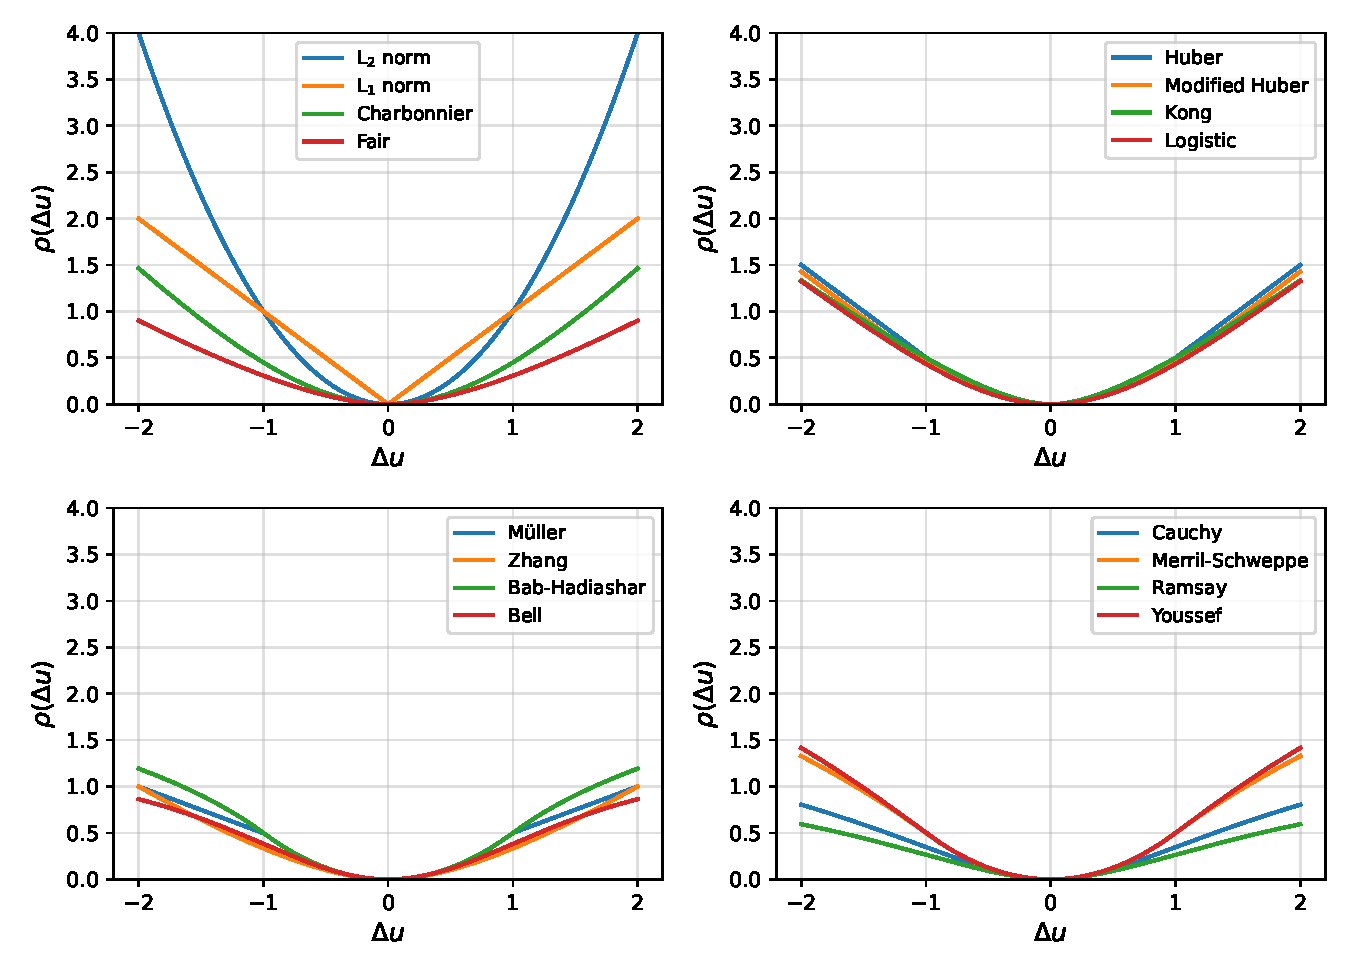
\includegraphics[width=0.8\linewidth]{figs/rho_functions.pdf}
\caption{Funkcje $\rho(\Delta u)$ dla $c=1$ (odpowiednik rys.~2 z~ICCMA 2024).}
\label{fig:rho}
\end{figure}

\paragraph{Uwagi implementacyjne.}
\begin{itemize}
\item Funkcja L$_1$ jest nieróżniczkowalna w~zerze, dlatego NMPC-L$_1$ rozwiązywany jest
w~postaci równoważnej z~dodatkowymi zmiennymi $s_r\ge|\Delta u_r|$ (minimalizacja $R\sum s_r$),
co daje zadanie gładkie dla SLSQP. Pozostałe funkcje są klasy co najmniej $C^1$.
\item Ograniczenia $u_\mathrm{min}\le u(k+p|k)\le u_\mathrm{max}$ nałożono na skumulowane
sterowanie (w~pracy inżynierskiej ograniczane były pojedyncze przyrosty). W~badanych scenariuszach
ograniczenia nie są aktywne ($|u|<10$~N).
\item Tolerancję solvera zaostrzono do $10^{-8}$; przy $10^{-4}$ solver kończył obliczenia przed
osiągnięciem minimum, co zaburzałoby porównanie funkcji kosztu. Wynik NMPC-L$_2$ w~scenariuszu
nominalnym pokrywa się z~pracą inżynierską (IAE$_\theta$: $0{,}02325$ vs.~$0{,}02323$).
\item Regulatory LQR (dyskretny, DLQR) oraz LQR-I (DLQR z~całkowaniem uchybu położenia)
dostrojono tym samym algorytmem ewolucji różnicowej i~tym samym kryterium co pozostałe regulatory
w~pracy (scenariusz nominalny).
\item Wskaźniki liczone są zgodnie z~artykułem dla $k=1,\ldots,N_s$; $K_\mathrm{VT}$ z~$u(0)=0$.
\end{itemize}

\section{Scenariusze}

\paragraph{S1 -- nominalny} (jak w~pracy inżynierskiej): $x(0)=[0{,}05;\,0;\,0;\,0]^T$,
$x_\mathrm{ref}=[0;\,0;\,0{,}1;\,0]^T$, $T=10$~s ($N_s=100$), brak zakłócenia.

\paragraph{S2 -- skoki zakłócenia.} Układ startuje z~położenia równowagi
($x(0)=x_\mathrm{ref}=0$), a~siła $F_\mathrm{w}$ zmienia się skokowo:
$F_\mathrm{w}=0$ dla $t<2$~s, następnie $F_\mathrm{w}=0.05$~N od $t=2$~s; $F_\mathrm{w}=-0.1$~N od $t=22$~s; $F_\mathrm{w}=0.08$~N od $t=42$~s; $F_\mathrm{w}=-0.04$~N od $t=62$~s.

Każda wartość utrzymywana jest przez 20~s, tak aby wszystkie regulatory zdążyły ustalić
przebiegi przed kolejną zmianą; $T=82$~s ($N_s=820$).

\paragraph{Ważna uwaga dot. scenariusza S2 (prośba o decyzję).}
Przy stałej sile $F_\mathrm{w}$ działającej na końcu wahadła położenie $\theta=0$ \emph{nie jest}
punktem równowagi. Z~równań ruchu (przy $\ddot\theta=\ddot x_\mathrm{p}=0$) wynika
\begin{equation}
\tan\theta_\mathrm{ss}=-\frac{F_\mathrm{w}}{mg},\qquad u_\mathrm{ss}\approx -F_\mathrm{w},
\end{equation}
czyli ok.~$0{,}44$~rad na każdy 1~N zakłócenia ($m=0{,}23$~kg). Żaden regulator nie sprowadzi
więc kąta do zera -- kąt zbiega do $\theta_\mathrm{ss}$ (linia przerywana na wykresach), a~do
zera może wrócić jedynie położenie wózka, i~to tylko w~regulatorach z~całkowaniem. Z~tego powodu:
\begin{itemize}
\item amplitudy dobrano małe ($0{,}04$--$0{,}1$~N, $|\theta_\mathrm{ss}|\le 2{,}5^\circ$), rzędu
zakłócenia z~pracy inżynierskiej; przy $0{,}3$--$0{,}5$~N NMPC-L$_2$ tracił stabilność, a~wózek
przemieszczał się o~kilka metrów;
\item wskaźniki $\mathrm{MSE}_\theta$ i~$\mathrm{MAE}_\theta$ liczone względem $\theta_\mathrm{ref}=0$
zawierają składnik wynikający z~$\theta_\mathrm{ss}\neq0$, jednakowy dla wszystkich stabilnych
regulatorów -- różnice między algorytmami wynikają ze stanów przejściowych;
\item \textbf{pytanie:} czy pozostawić taką postać scenariusza, czy zastosować np.~impulsy
prostokątne (zakłócenie pojawia się i~znika, po każdym impulsie układ wraca do zera)?
\end{itemize}

\section{Parametry regulatorów}
\begin{table}[H]\centering\small
\caption{Parametry wszystkich regulatorów (takie same w~obu scenariuszach).}
\begin{tabular}{lp{12.5cm}}
\hline
Algorytm & Parametry \\
\hline
PID & $K_{p,\theta}=-40$, $K_{i,\theta}=-1$, $K_{d,\theta}=-8$; $K_{p,x}=-1$, $K_{i,x}=-0.1$, $K_{d,x}=-3$; $I_{\max}=5$ \\
LQR & $Q=\mathrm{diag}(437.398, 56.197, 378.065, 77.873)$, $R=8.3412$ \\
LQR-I & $\tilde{Q}=\mathrm{diag}(148.887, 51.76, 326.26, 41.484, 0.06)$, $R=5.9162$ \\
PID-LQR & $Q=\mathrm{diag}(200, 3, 35, 40)$, $R=1$; $K_{p,x}=-7$, $K_{i,x}=0.1$, $K_{d,x}=-3$ \\
Fuzzy-LQR & $K_\mathrm{base}=[40,1,15,20]$, przyrosty $[20,5,5,2]\cdot L_i$, $G=0.36$, $K_\mathrm{LQR}$: $Q=I$, $R=1$ \\
LMPC & $N=12$, $N_\mathrm{u}=4$, $Q=\mathrm{diag}(15, 1, 15, 1)$, $R=0.1$ \\
MPC-NO-alt & $N=12$, $N_\mathrm{u}=4$, $Q$ jak NMPC, $R=0.001$, $R_\mathrm{abs}=1$ \\
NMPC-$\rho$ & $N=12$, $N_\mathrm{u}=4$, $Q=\mathrm{diag}(158.39, 40.8, 43.41, 19.71)$, $R=0.08592$, $c=1$ (wszystkie $\rho$) \\
\hline
\end{tabular}

\end{table}

\section{Wyniki}
Oznaczenia: $^{\dagger}$ -- niestabilny ($|\theta|>\pi/4$ lub $|x_\mathrm{p}|>5$~m),
$^{\ddagger}$ -- przebiegi nieustalone na końcu odcinka (automatyczny test; każdy przebieg
przejrzano dodatkowo na wykresach w~dodatku). Pogrubiono najlepszą wartość wśród regulatorów
stabilnych.

\begin{table}[H]\centering\small
\caption{Scenariusz S1 (nominalny) -- wskaźniki jakości regulacji.}
\begin{tabular}{lccccc}
\hline
Algorytm & $\mathrm{MSE}_\theta$ & $\mathrm{MSE}_{x}$ & $\mathrm{MAE}_\theta$ & $\mathrm{MAE}_{x}$ & $K_\mathrm{VT}$ \\
\hline
PID & $9.0106\times10^{-5}$ & $4.1321\times10^{-4}$ & $4.3166\times10^{-3}$ & $9.2272\times10^{-3}$ & $6.2037\times10^{0}$ \\
LQR & $3.9429\times10^{-5}$ & $2.9443\times10^{-4}$ & $2.1989\times10^{-3}$ & $6.5523\times10^{-3}$ & $5.9039\times10^{0}$ \\
LQR-I & $4.0409\times10^{-5}$ & $2.9437\times10^{-4}$ & $2.2412\times10^{-3}$ & $6.5835\times10^{-3}$ & $5.8794\times10^{0}$ \\
PID-LQR & $6.7870\times10^{-5}$ & {\boldmath$2.6266\times10^{-4}$} & $2.9192\times10^{-3}$ & {\boldmath$4.7626\times10^{-3}$} & $6.4254\times10^{0}$ \\
Fuzzy-LQR & {\boldmath$2.1039\times10^{-5}$} & $3.3592\times10^{-4}$ & {\boldmath$1.3281\times10^{-3}$} & $7.0909\times10^{-3}$ & $8.6180\times10^{0}$ \\
LMPC & $5.8548\times10^{-5}$ & $2.9099\times10^{-4}$ & $2.7274\times10^{-3}$ & $5.9994\times10^{-3}$ & {\boldmath$5.3416\times10^{0}$} \\
MPC-NO-alt & $4.2428\times10^{-5}$ & $6.4375\times10^{-4}$ & $2.5933\times10^{-3}$ & $1.5104\times10^{-2}$ & $5.5643\times10^{0}$ \\
\hline
NMPC-L$_2$ & $3.7601\times10^{-5}$ & $2.8385\times10^{-4}$ & $2.0748\times10^{-3}$ & $6.2407\times10^{-3}$ & $5.9593\times10^{0}$ \\
NMPC-L$_1$ & $3.1676\times10^{-5}$ & $2.9340\times10^{-4}$ & $1.9294\times10^{-3}$ & $7.3746\times10^{-3}$ & $6.4607\times10^{0}$ \\
NMPC-Ch & $3.3061\times10^{-5}$ & $2.7877\times10^{-4}$ & $1.9139\times10^{-3}$ & $5.7167\times10^{-3}$ & $6.4285\times10^{0}$ \\
NMPC-F & $3.2149\times10^{-5}$ & $2.7859\times10^{-4}$ & $1.8823\times10^{-3}$ & $5.6326\times10^{-3}$ & $6.5360\times10^{0}$ \\
NMPC-Hu & $3.2656\times10^{-5}$ & $2.7879\times10^{-4}$ & $1.9012\times10^{-3}$ & $5.6901\times10^{-3}$ & $6.4831\times10^{0}$ \\
NMPC-MH & $3.2658\times10^{-5}$ & $2.7877\times10^{-4}$ & $1.9010\times10^{-3}$ & $5.6889\times10^{-3}$ & $6.4813\times10^{0}$ \\
NMPC-K & $3.2395\times10^{-5}$ & $2.7966\times10^{-4}$ & $1.8969\times10^{-3}$ & $5.7563\times10^{-3}$ & $6.5076\times10^{0}$ \\
NMPC-L & $3.2629\times10^{-5}$ & $2.7876\times10^{-4}$ & $1.8999\times10^{-3}$ & $5.6859\times10^{-3}$ & $6.4840\times10^{0}$ \\
NMPC-M & $3.1720\times10^{-5}$ & $2.7891\times10^{-4}$ & $1.8710\times10^{-3}$ & $5.6246\times10^{-3}$ & $6.6032\times10^{0}$ \\
NMPC-Z & $3.2308\times10^{-5}$ & $2.7861\times10^{-4}$ & $1.8879\times10^{-3}$ & $5.6469\times10^{-3}$ & $6.5185\times10^{0}$ \\
NMPC-BH & $3.1494\times10^{-5}$ & $2.7896\times10^{-4}$ & $1.8636\times10^{-3}$ & $5.6101\times10^{-3}$ & $6.6313\times10^{0}$ \\
NMPC-Be & $3.1130\times10^{-5}$ & $2.7903\times10^{-4}$ & $1.8512\times10^{-3}$ & $5.5844\times10^{-3}$ & $6.6773\times10^{0}$ \\
NMPC-C & $3.1405\times10^{-5}$ & $2.7893\times10^{-4}$ & $1.8599\times10^{-3}$ & $5.5983\times10^{-3}$ & $6.6404\times10^{0}$ \\
NMPC-MS & $3.1951\times10^{-5}$ & $2.7887\times10^{-4}$ & $1.8784\times10^{-3}$ & $5.6417\times10^{-3}$ & $6.5735\times10^{0}$ \\
NMPC-R & $3.1151\times10^{-5}$ & $2.7885\times10^{-4}$ & $1.8498\times10^{-3}$ & $5.5737\times10^{-3}$ & $6.6720\times10^{0}$ \\
NMPC-Y & $3.2054\times10^{-5}$ & $2.7884\times10^{-4}$ & $1.8816\times10^{-3}$ & $5.6448\times10^{-3}$ & $6.5537\times10^{0}$ \\
\hline
\end{tabular}

\end{table}

\begin{table}[H]\centering\small
\caption{Scenariusz S2 (skoki zakłócenia) -- wskaźniki jakości regulacji.}
\begin{tabular}{lccccc}
\hline
Algorytm & $\mathrm{MSE}_\theta$ & $\mathrm{MSE}_{x}$ & $\mathrm{MAE}_\theta$ & $\mathrm{MAE}_{x}$ & $K_\mathrm{VT}$ \\
\hline
PID$^{\ddagger}$ & $1.4917\times10^{-3}$ & $7.9974\times10^{-1}$ & $3.3805\times10^{-2}$ & $8.0837\times10^{-1}$ & $4.5189\times10^{1}$ \\
LQR & $1.2553\times10^{-3}$ & $2.4147\times10^{-1}$ & $3.1871\times10^{-2}$ & $4.5067\times10^{-1}$ & $3.0611\times10^{1}$ \\
LQR-I & $1.2569\times10^{-3}$ & $2.0326\times10^{-1}$ & $3.1831\times10^{-2}$ & $4.1144\times10^{-1}$ & $3.1312\times10^{1}$ \\
PID-LQR & $1.2265\times10^{-3}$ & {\boldmath$3.1605\times10^{-2}$} & $3.1055\times10^{-2}$ & {\boldmath$1.6441\times10^{-1}$} & $4.7860\times10^{1}$ \\
Fuzzy-LQR & {\boldmath$1.1225\times10^{-3}$} & $8.5151\times10^{-2}$ & {\boldmath$3.0700\times10^{-2}$} & $2.6998\times10^{-1}$ & $2.9667\times10^{1}$ \\
LMPC & $1.3070\times10^{-3}$ & $1.3639\times10^{-1}$ & $3.2062\times10^{-2}$ & $3.4019\times10^{-1}$ & $3.8344\times10^{1}$ \\
MPC-NO-alt & $1.3821\times10^{-3}$ & $9.8628\times10^{-1}$ & $3.3140\times10^{-2}$ & $9.0420\times10^{-1}$ & $2.9237\times10^{1}$ \\
\hline
NMPC-L$_2$ & $1.2135\times10^{-3}$ & $2.9621\times10^{-1}$ & $3.1623\times10^{-2}$ & $4.9686\times10^{-1}$ & $2.9090\times10^{1}$ \\
NMPC-L$_1$ & $1.1733\times10^{-3}$ & $2.3180\times10^{-1}$ & $3.1242\times10^{-2}$ & $4.4176\times10^{-1}$ & $3.2535\times10^{1}$ \\
NMPC-Ch & $1.1820\times10^{-3}$ & $2.3917\times10^{-1}$ & $3.1321\times10^{-2}$ & $4.4810\times10^{-1}$ & $2.7315\times10^{1}$ \\
NMPC-F & $1.1762\times10^{-3}$ & $2.2951\times10^{-1}$ & $3.1261\times10^{-2}$ & $4.3852\times10^{-1}$ & $2.7343\times10^{1}$ \\
NMPC-Hu & $1.1802\times10^{-3}$ & $2.3696\times10^{-1}$ & $3.1306\times10^{-2}$ & $4.4706\times10^{-1}$ & $2.7235\times10^{1}$ \\
NMPC-MH & $1.1800\times10^{-3}$ & $2.3630\times10^{-1}$ & $3.1303\times10^{-2}$ & $4.4597\times10^{-1}$ & {\boldmath$2.7196\times10^{1}$} \\
NMPC-K & $1.1776\times10^{-3}$ & $2.3292\times10^{-1}$ & $3.1279\times10^{-2}$ & $4.4238\times10^{-1}$ & $2.7233\times10^{1}$ \\
NMPC-L & $1.1795\times10^{-3}$ & $2.3531\times10^{-1}$ & $3.1296\times10^{-2}$ & $4.4468\times10^{-1}$ & $2.7208\times10^{1}$ \\
NMPC-M & $1.1729\times10^{-3}$ & $2.2662\times10^{-1}$ & $3.1233\times10^{-2}$ & $4.3682\times10^{-1}$ & $3.5598\times10^{1}$ \\
NMPC-Z & $1.1772\times10^{-3}$ & $2.3115\times10^{-1}$ & $3.1271\times10^{-2}$ & $4.4016\times10^{-1}$ & $2.7280\times10^{1}$ \\
NMPC-BH & $1.1737\times10^{-3}$ & $2.2769\times10^{-1}$ & $3.1243\times10^{-2}$ & $4.3912\times10^{-1}$ & $2.7588\times10^{1}$ \\
NMPC-Be & $1.1710\times10^{-3}$ & $2.2287\times10^{-1}$ & $3.1212\times10^{-2}$ & $4.3338\times10^{-1}$ & $2.7550\times10^{1}$ \\
NMPC-C & $1.1719\times10^{-3}$ & $2.2388\times10^{-1}$ & $3.1220\times10^{-2}$ & $4.3377\times10^{-1}$ & $2.7561\times10^{1}$ \\
NMPC-MS & $1.1764\times10^{-3}$ & $2.3144\times10^{-1}$ & $3.1269\times10^{-2}$ & $4.4240\times10^{-1}$ & $2.7328\times10^{1}$ \\
NMPC-R & $1.1705\times10^{-3}$ & $2.2131\times10^{-1}$ & $3.1204\times10^{-2}$ & $4.3096\times10^{-1}$ & $2.7662\times10^{1}$ \\
NMPC-Y & $1.1773\times10^{-3}$ & $2.3290\times10^{-1}$ & $3.1279\times10^{-2}$ & $4.4381\times10^{-1}$ & $2.7236\times10^{1}$ \\
\hline
\end{tabular}

\end{table}

\begin{table}[H]\centering\small
\caption{Status stabilności (test automatyczny), wartości maksymalne w~S2 i~liczba niepowodzeń solvera (S1+S2).}
\resizebox{\linewidth}{!}{\begin{tabular}{lccccc}
\hline
Algorytm & status S1 & status S2 & $\max|u|$ S2 [N] & $\max|x_\mathrm{p}|$ S2 [m] & niepowodzenia solvera \\
\hline
PID & stabilny & nieustalony & 4.72 & 1.490 & -- \\
LQR & stabilny & stabilny & 4.07 & 0.733 & -- \\
LQR-I & stabilny & stabilny & 4.08 & 0.738 & -- \\
PID-LQR & stabilny & stabilny & 4.52 & 0.301 & -- \\
Fuzzy-LQR & stabilny & stabilny & 4.31 & 0.421 & -- \\
LMPC & stabilny & stabilny & 4.71 & 0.562 & 0/920 \\
MPC-NO-alt & stabilny & stabilny & 3.95 & 1.514 & 0/920 \\
NMPC-L$_2$ & stabilny & stabilny & 4.06 & 0.810 & 0/920 \\
NMPC-L$_1$ & stabilny & stabilny & 3.92 & 0.714 & 0/920 \\
NMPC-Ch & stabilny & stabilny & 3.80 & 0.722 & 0/920 \\
NMPC-F & stabilny & stabilny & 3.85 & 0.709 & 0/920 \\
NMPC-Hu & stabilny & stabilny & 3.79 & 0.715 & 0/920 \\
NMPC-MH & stabilny & stabilny & 3.79 & 0.716 & 0/920 \\
NMPC-K & stabilny & stabilny & 3.83 & 0.712 & 0/920 \\
NMPC-L & stabilny & stabilny & 3.80 & 0.715 & 0/920 \\
NMPC-M & stabilny & stabilny & 3.90 & 0.702 & 0/920 \\
NMPC-Z & stabilny & stabilny & 3.84 & 0.711 & 0/920 \\
NMPC-BH & stabilny & stabilny & 3.89 & 0.699 & 0/920 \\
NMPC-Be & stabilny & stabilny & 3.93 & 0.695 & 0/920 \\
NMPC-C & stabilny & stabilny & 3.92 & 0.698 & 0/920 \\
NMPC-MS & stabilny & stabilny & 3.84 & 0.706 & 0/920 \\
NMPC-R & stabilny & stabilny & 3.94 & 0.695 & 0/920 \\
NMPC-Y & stabilny & stabilny & 3.82 & 0.707 & 0/920 \\
\hline
\end{tabular}
}
\end{table}

\subsection{Obserwacje}

\paragraph{Stabilność.} Wszystkie 23 algorytmy działają poprawnie w~obu scenariuszach -- żaden
nie stracił stabilności, a~solver nie zgłosił ani jednego niepowodzenia. Jedyny przypadek
oznaczony jako nieustalony to PID w~S2: integrator pętli kąta nie może sprowadzić uchybu
$\theta$ do zera (bo $\theta_\mathrm{ss}\neq0$), nasyca się i~wózek dryfuje
($|x_\mathrm{p}|$ do $1{,}5$~m). Dwa algorytmy NMPC działają, ale z~wadą widoczną dopiero na
przebiegach (rys.~w~dodatku):
\begin{itemize}
\item \textbf{NMPC-L$_1$} -- w~stanie ustalonym utrzymują się drobne oscylacje sterowania
($|\Delta u|\approx0{,}07$~N) i~kąta, co podnosi $K_\mathrm{VT}$ w~S2 o~ok.~12\% względem
NMPC-L$_2$. Funkcja $|\Delta u|$ jest nieróżniczkowalna w~zerze, czyli dokładnie w~punkcie,
w~którym leży rozwiązanie w~stanie ustalonym. Zgadza się to ze słabymi wynikami NMPC-L$_1$
w~ICCMA 2024 oraz z~[Karamanakos i~in. 2018].
\item \textbf{NMPC-M} (Müller) -- oscylacje ($|\Delta u|\approx0{,}11$~N) w~ostatnim odcinku S2,
$K_\mathrm{VT}$ większe o~22\%. Funkcja (12) ma w~$|\Delta u|=c$ skok pochodnej (z~$c$ na
$c/2$). Ponieważ model predykcji nie zna zakłócenia, regulator planuje w~dalszej części
horyzontu przyrosty $|\Delta u|\approx1=c$, a~więc dokładnie w~punkcie załamania, i~SLSQP
przeskakuje między jego stronami. Huber, równy Müllerowi dla $|\Delta u|\le c$, ma ciągłą
pochodną i~nie oscyluje. Zmiana tolerancji solvera ($10^{-8}$--$10^{-12}$) nie usuwa efektu.
\end{itemize}

\paragraph{S1 -- wpływ funkcji kosztu.} Wszystkie 15 alternatywnych funkcji daje mniejsze
$\mathrm{MSE}_\theta$ (o~12--17\%) i~$\mathrm{MAE}_\theta$ (o~7--11\%) niż NMPC-L$_2$, kosztem
większego $K_\mathrm{VT}$ (o~8--12\%). Przyczyną jest pierwszy, duży ruch sterowania
($|\Delta u|\approx2{,}5$--$3$~N), dla którego funkcje odporne rosną wolniej niż kwadratowa --
duży przyrost jest ,,tańszy'' i~regulator reaguje mocniej ($u(0)=2{,}95$~N dla NMPC-R
i~NMPC-Be wobec $2{,}55$~N dla NMPC-L$_2$). Jest to ten sam kompromis co w~ICCMA 2024 dla
reaktora pH (szybsza regulacja, większe $K_\mathrm{VT}$). Najmniejsze $\mathrm{MSE}_\theta$:
NMPC-Be, NMPC-R, NMPC-C; najmniejsze $K_\mathrm{VT}$ wśród alternatywnych: NMPC-Ch.
$\mathrm{MSE}_x$ jest prawie bez zmian (od $-2\%$ do $+3\%$, najgorsze NMPC-L$_1$).

\paragraph{S2 -- wpływ funkcji kosztu.} Tutaj alternatywne funkcje poprawiają
\emph{jednocześnie} wszystkie wskaźniki: $\mathrm{MSE}_x$ mniejsze o~19--25\%,
$\mathrm{MSE}_\theta$ o~3\% (mała różnica, bo dominuje wspólny składnik od $\theta_\mathrm{ss}$),
a~$K_\mathrm{VT}$ o~5--6\% -- z~wyjątkiem NMPC-L$_1$ i~NMPC-M opisanych wyżej. Najlepsze:
NMPC-R i~NMPC-Be ($\mathrm{MSE}_\theta$, $\mathrm{MSE}_x$), NMPC-MH ($K_\mathrm{VT}$).

\paragraph{Porównanie z~pozostałymi algorytmami.} Różnice między wariantami NMPC są
mniejsze niż różnice między klasami regulatorów. Fuzzy-LQR ma najmniejsze
$\mathrm{MSE}_\theta$ w~obu scenariuszach, ale największe $K_\mathrm{VT}$ w~S1. PID-LQR
najlepiej utrzymuje położenie wózka w~S2 (całkowanie w~pętli położenia przy dużych
wzmocnieniach), za to ma jedno z~największych $K_\mathrm{VT}$. LMPC ma najmniejsze
$K_\mathrm{VT}$ w~S1. Regulatory bez całkowania nie sprowadzają wózka do zera w~S2; LQR-I robi to
bardzo wolno, bo waga integratora dobrana na scenariuszu nominalnym jest mała ($0{,}06$).

\paragraph{Uwagi do dalszych prac (do decyzji).}
\begin{itemize}
\item Parametry kształtu $c=1$ przyjęto jak w~ICCMA 2024. W~tym obiekcie przyrosty sterowania
są rzędu 0,1--3~N, więc $c=1$ leży wewnątrz zakresu pracy (inaczej niż przy
przeskalowanych zmiennych w~reaktorze pH). Ewentualna analiza wrażliwości na $c$ -- do decyzji.
\item Czasy obliczeń nie są podawane: symulacje liczono równolegle, więc nie są miarodajne.
Mogę je zmierzyć osobno, jeśli będą potrzebne.
\end{itemize}


\section{Przebiegi reprezentatywne}
\begin{figure}[H]\centering
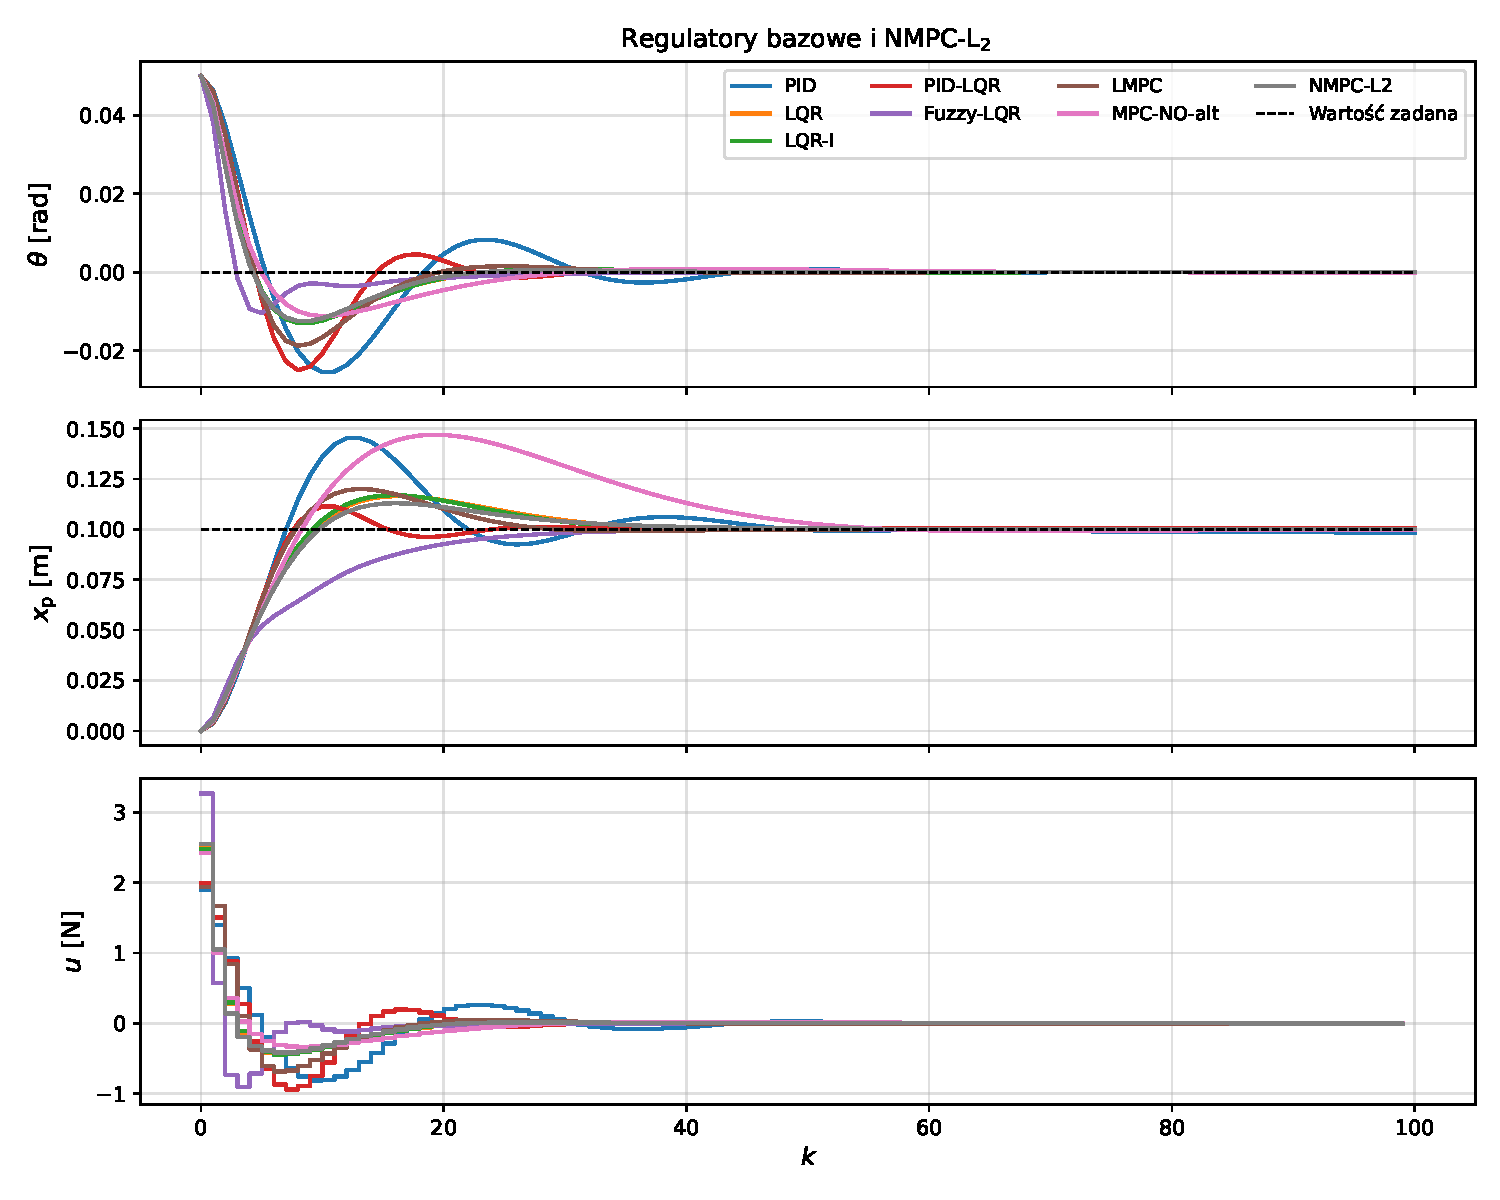
\includegraphics[width=0.9\linewidth]{figs/S1_compare_baseline.pdf}
\caption{S1: regulatory bazowe i~NMPC-L$_2$.}
\end{figure}
\begin{figure}[H]\centering
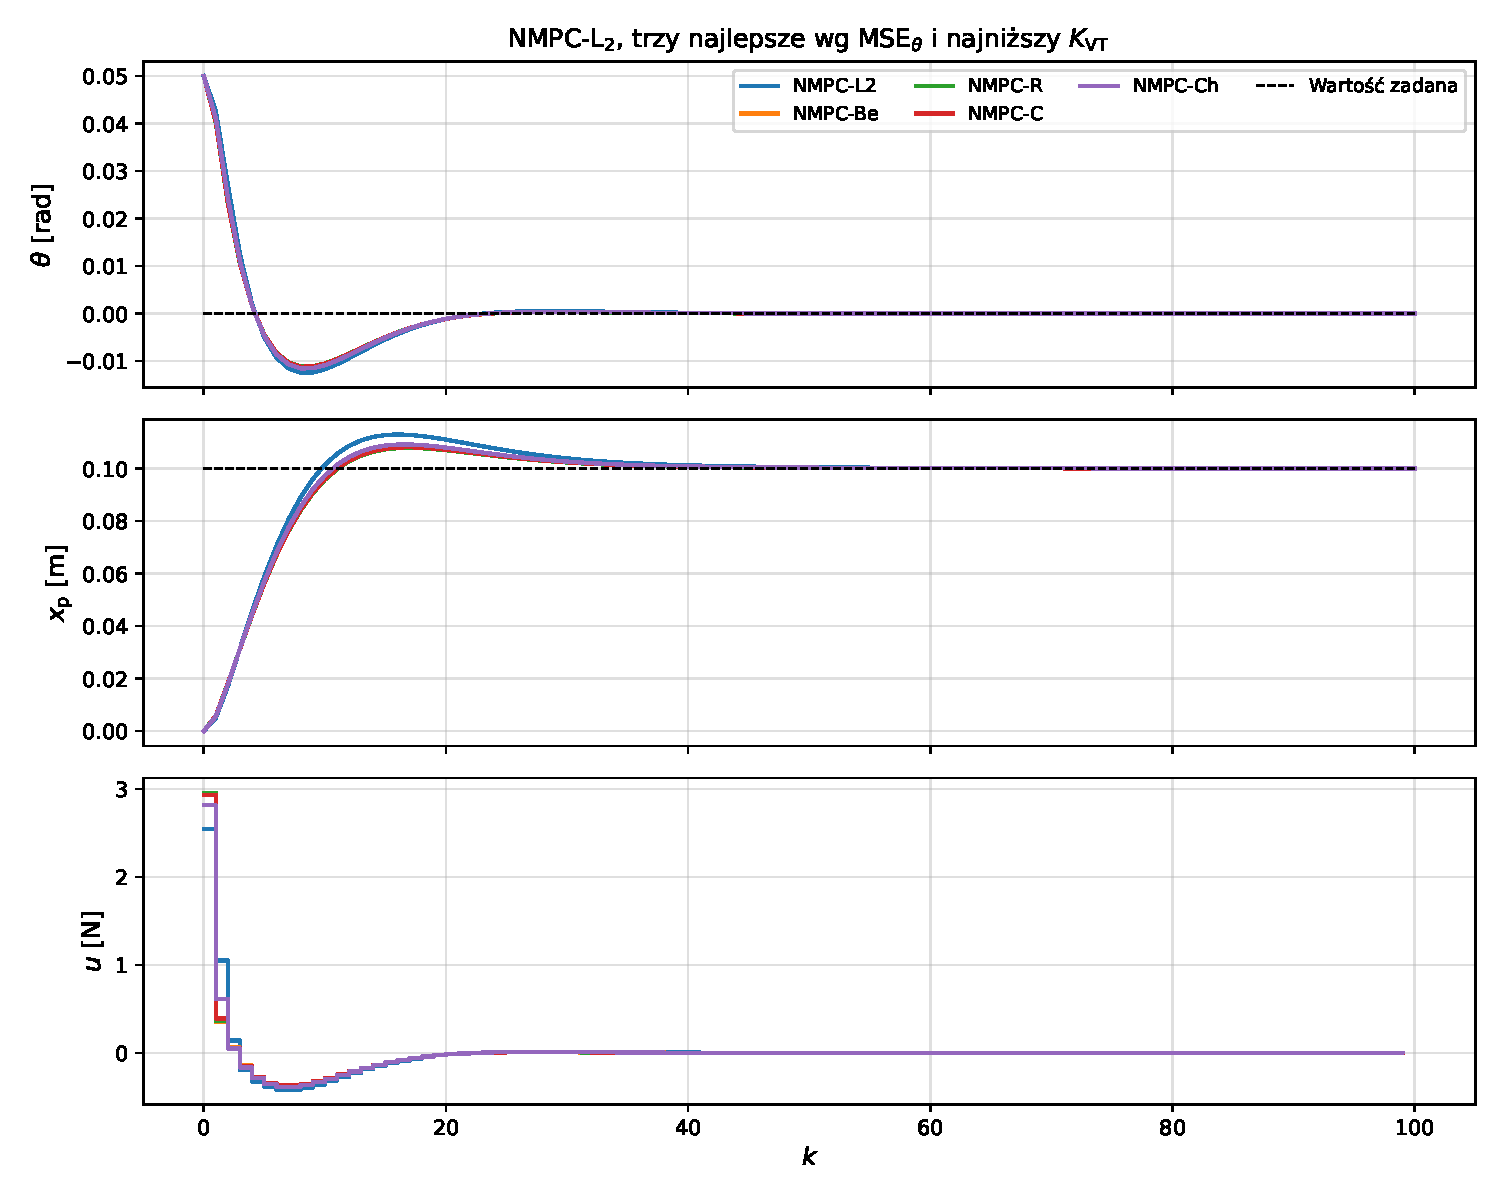
\includegraphics[width=0.9\linewidth]{figs/S1_compare_nmpc.pdf}
\caption{S1: \PickedSA.}
\end{figure}
\begin{figure}[H]\centering
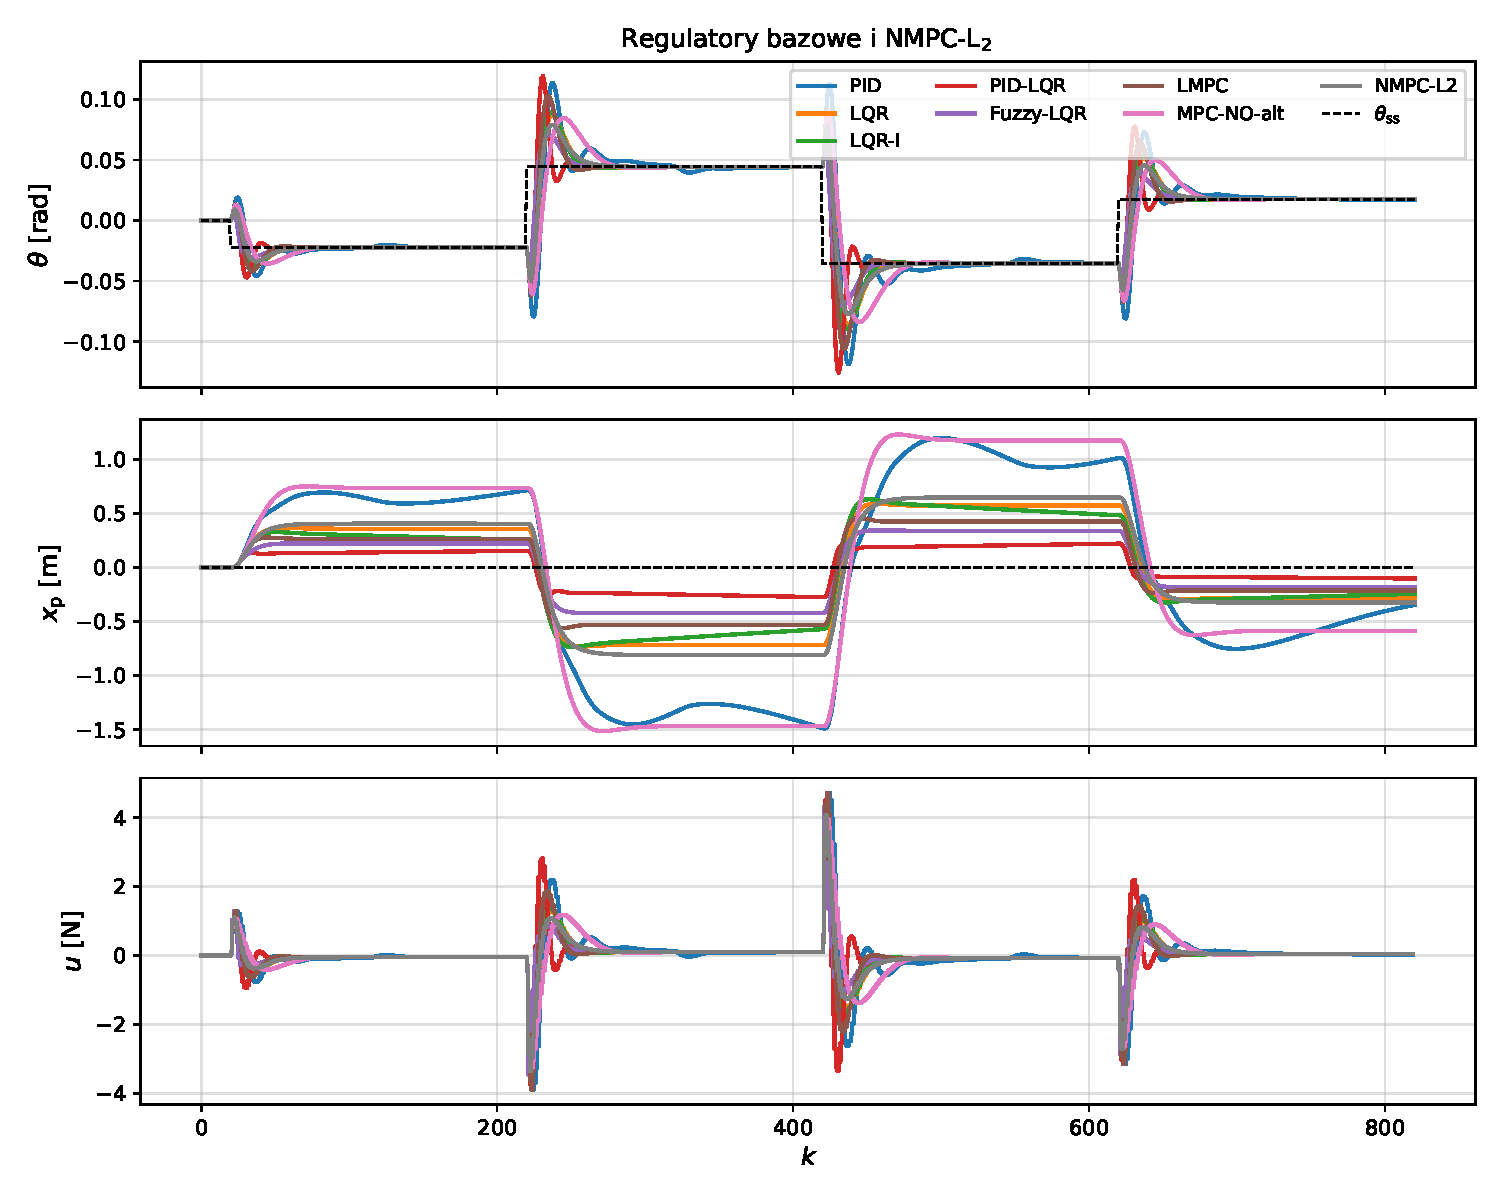
\includegraphics[width=0.9\linewidth]{figs/S2_compare_baseline.pdf}
\caption{S2: regulatory bazowe i~NMPC-L$_2$.}
\end{figure}
\begin{figure}[H]\centering
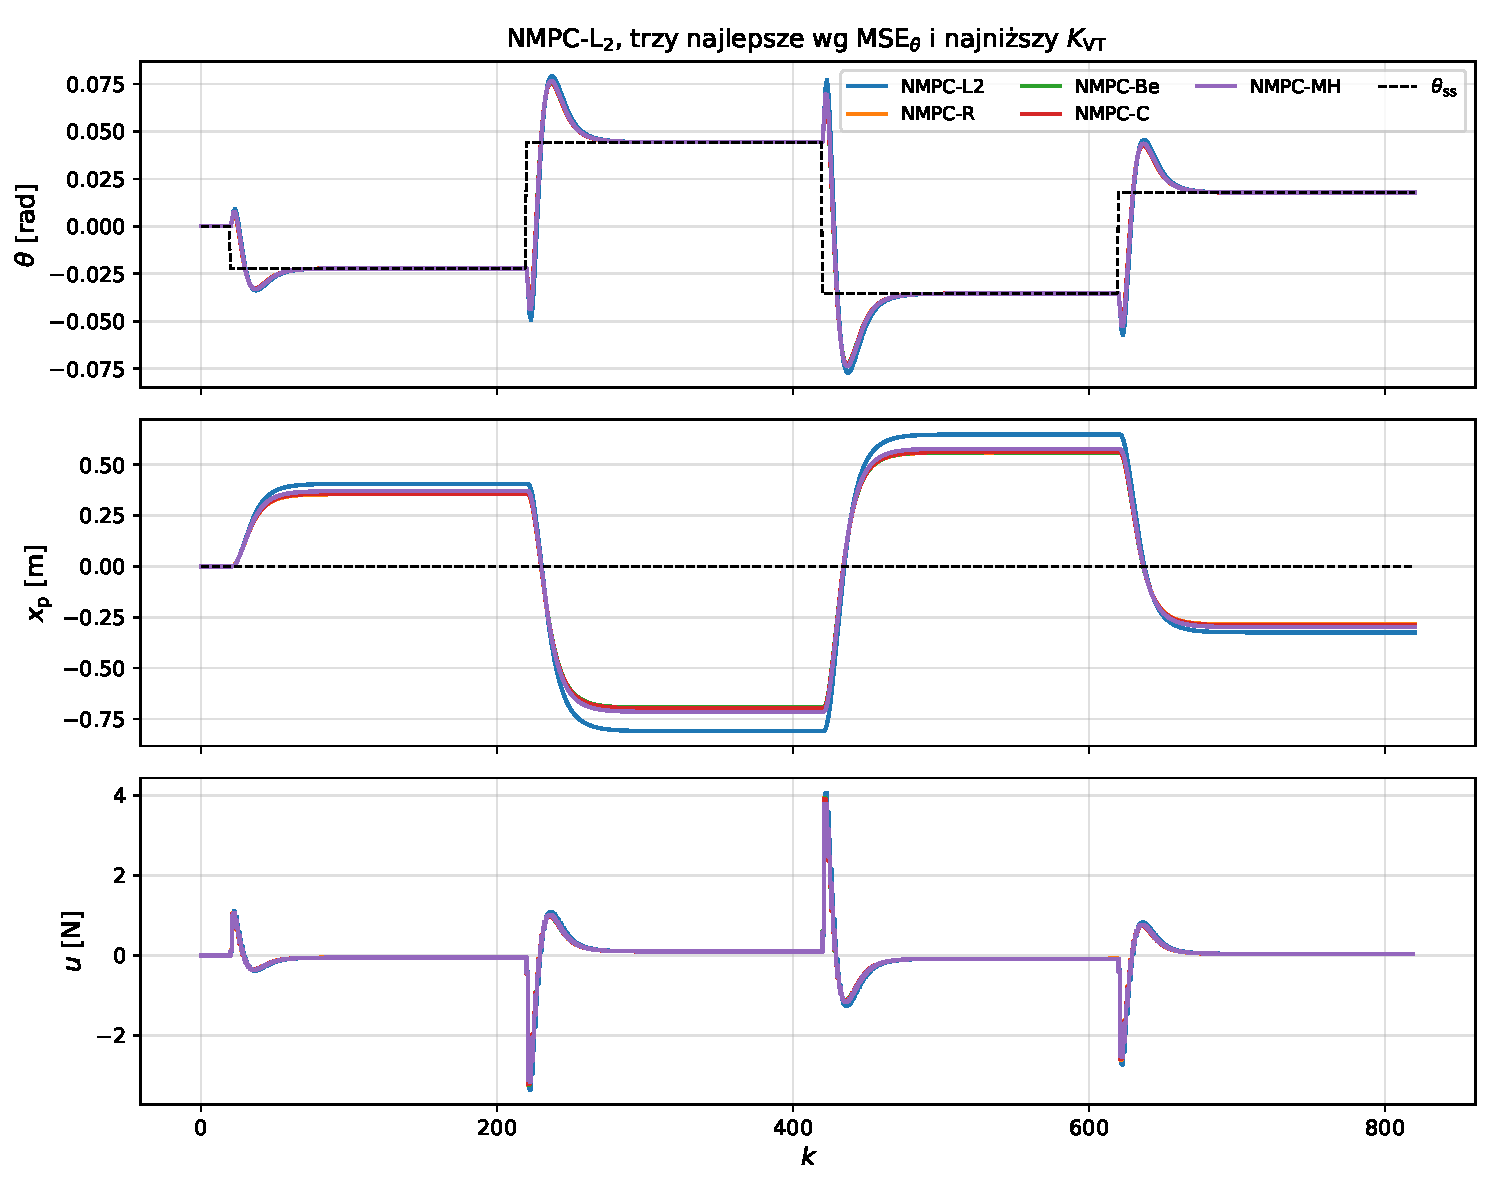
\includegraphics[width=0.9\linewidth]{figs/S2_compare_nmpc.pdf}
\caption{S2: \PickedSB.}
\end{figure}

\clearpage
\appendix
\section{Przebiegi wszystkich algorytmów (z~histogramami błędów i~sterowania)}
\subsection{Przebiegi -- Scenariusz S1 (nominalny)}
\begin{figure}[p]\centering
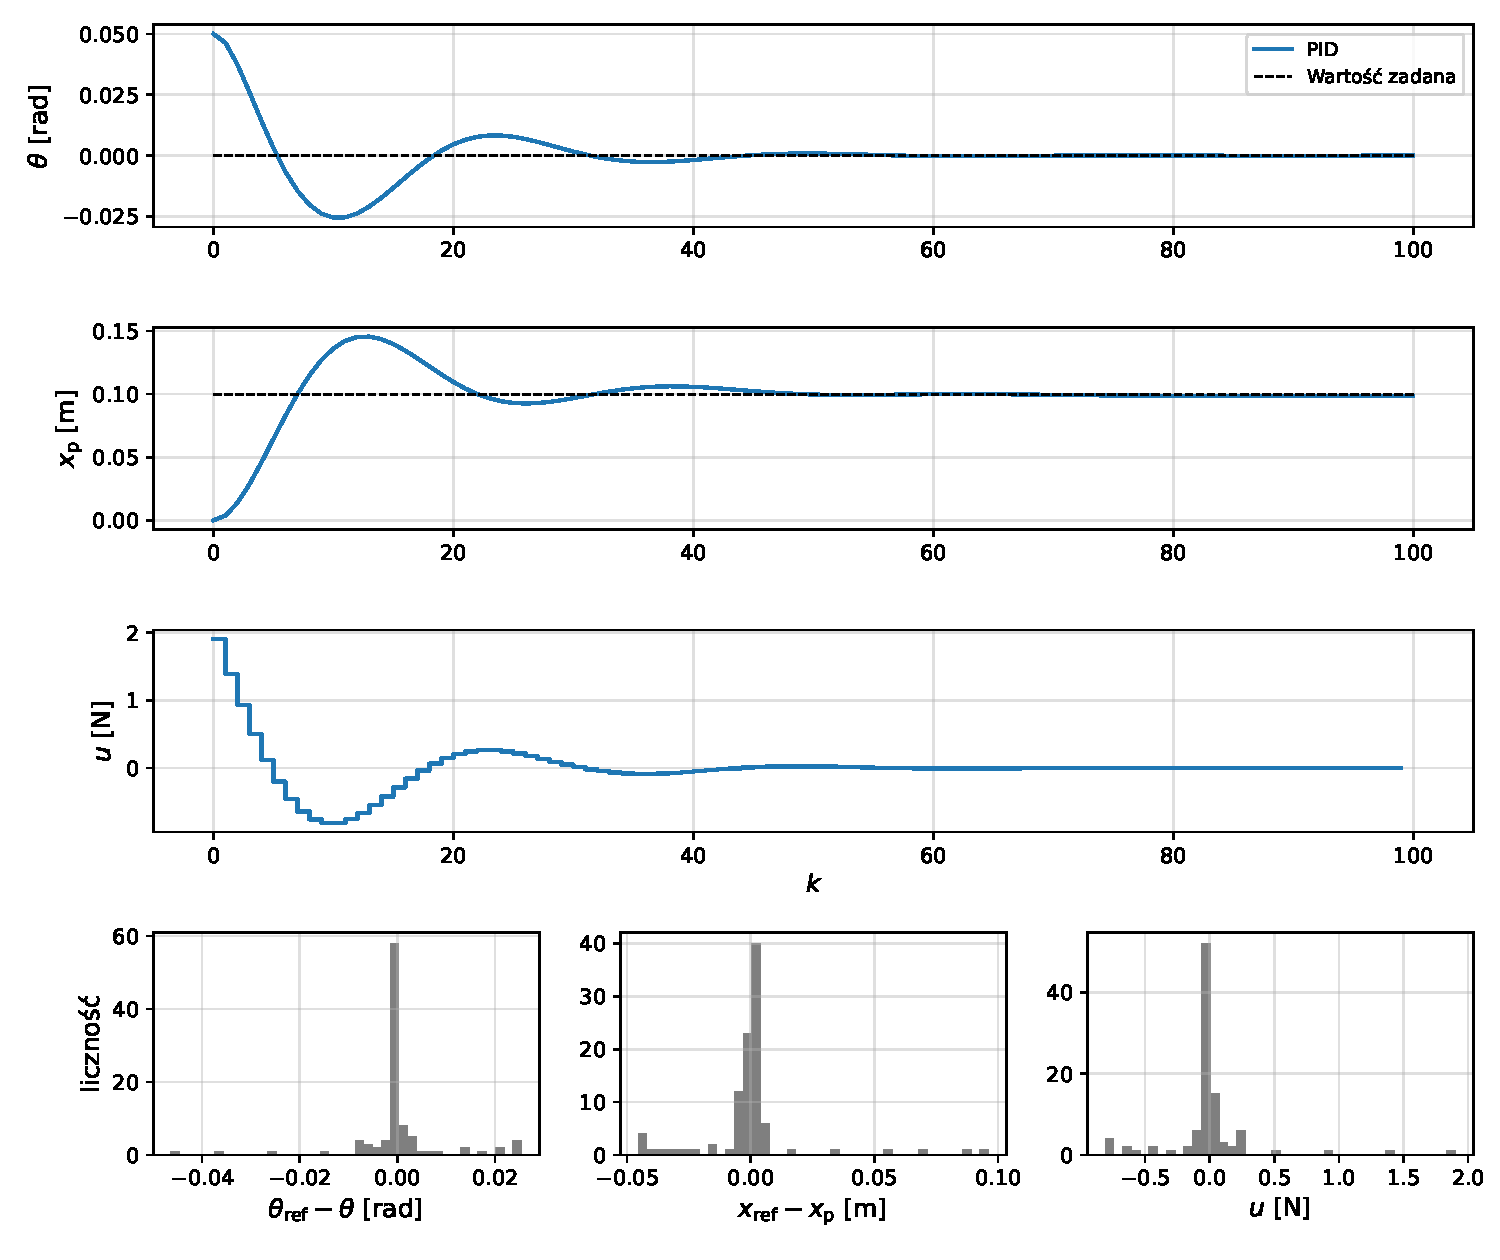
\includegraphics[width=\linewidth]{figs/S1_pid.pdf}
\caption{PID, Scenariusz S1 (nominalny): status automatyczny -- stabilny.}
\end{figure}
\clearpage
\begin{figure}[p]\centering
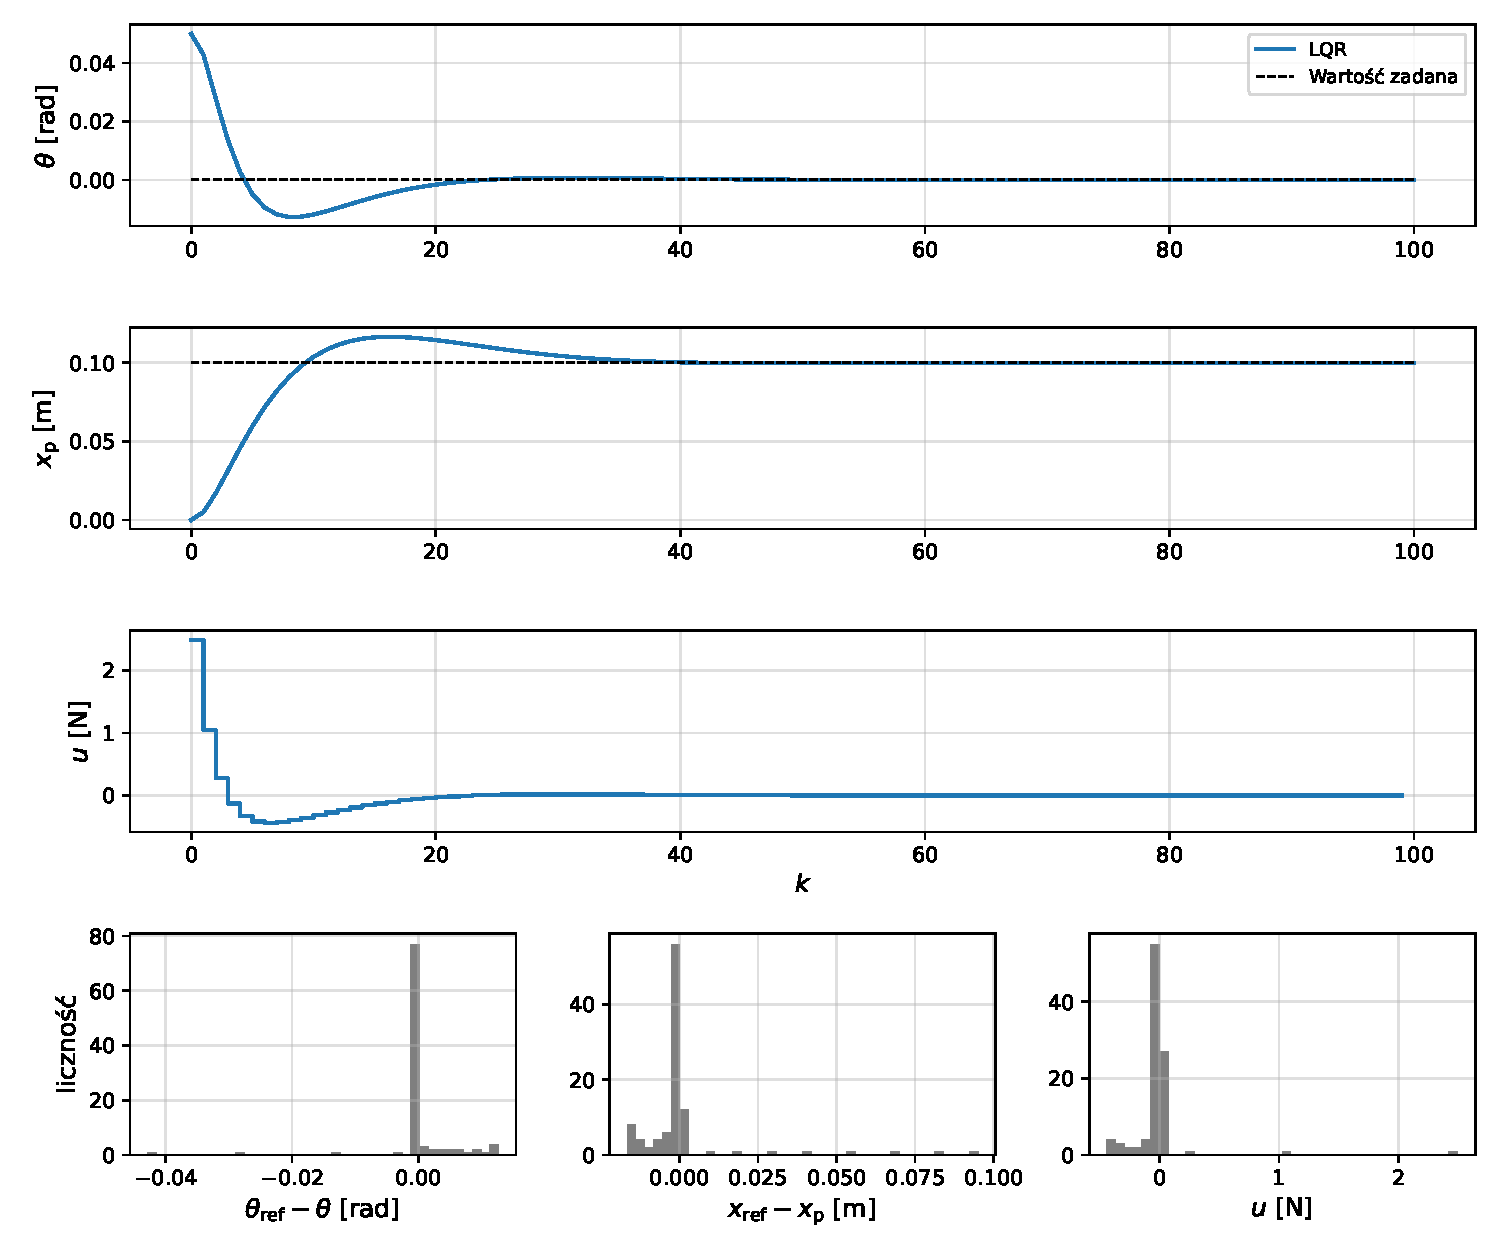
\includegraphics[width=\linewidth]{figs/S1_lqr.pdf}
\caption{LQR, Scenariusz S1 (nominalny): status automatyczny -- stabilny.}
\end{figure}
\clearpage
\begin{figure}[p]\centering
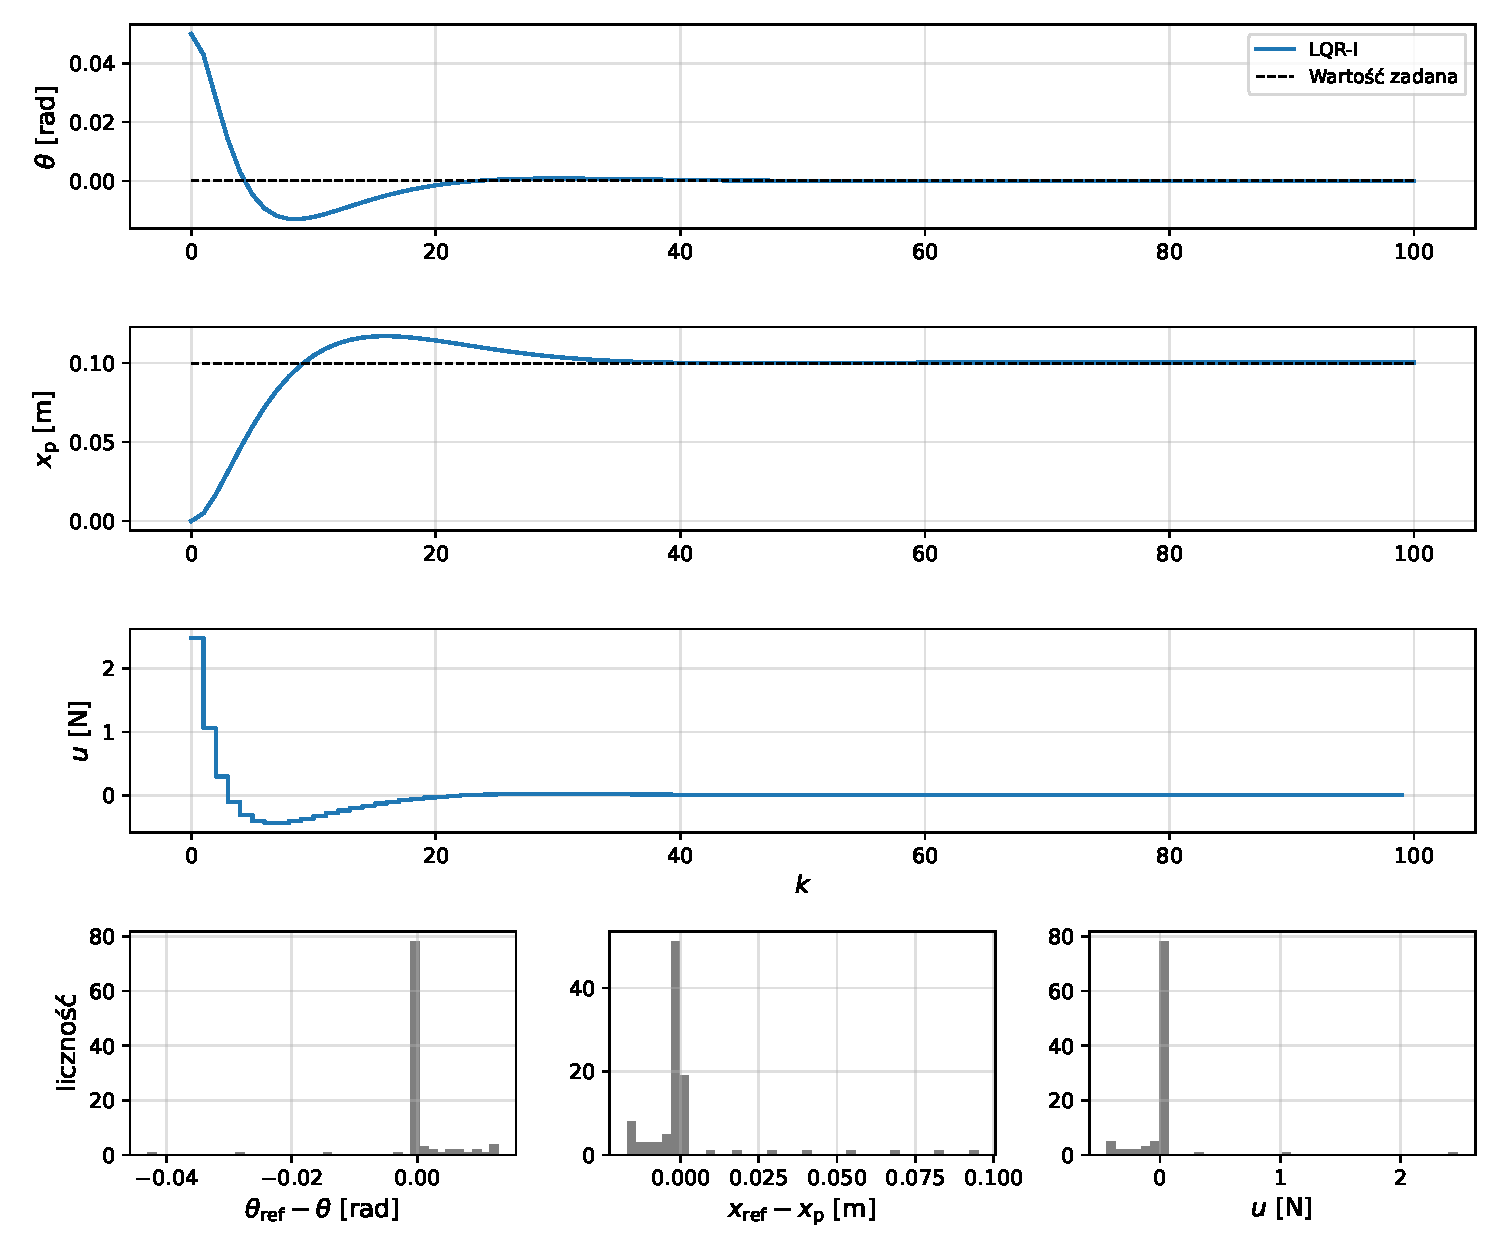
\includegraphics[width=\linewidth]{figs/S1_lqr_i.pdf}
\caption{LQR-I, Scenariusz S1 (nominalny): status automatyczny -- stabilny.}
\end{figure}
\clearpage
\begin{figure}[p]\centering
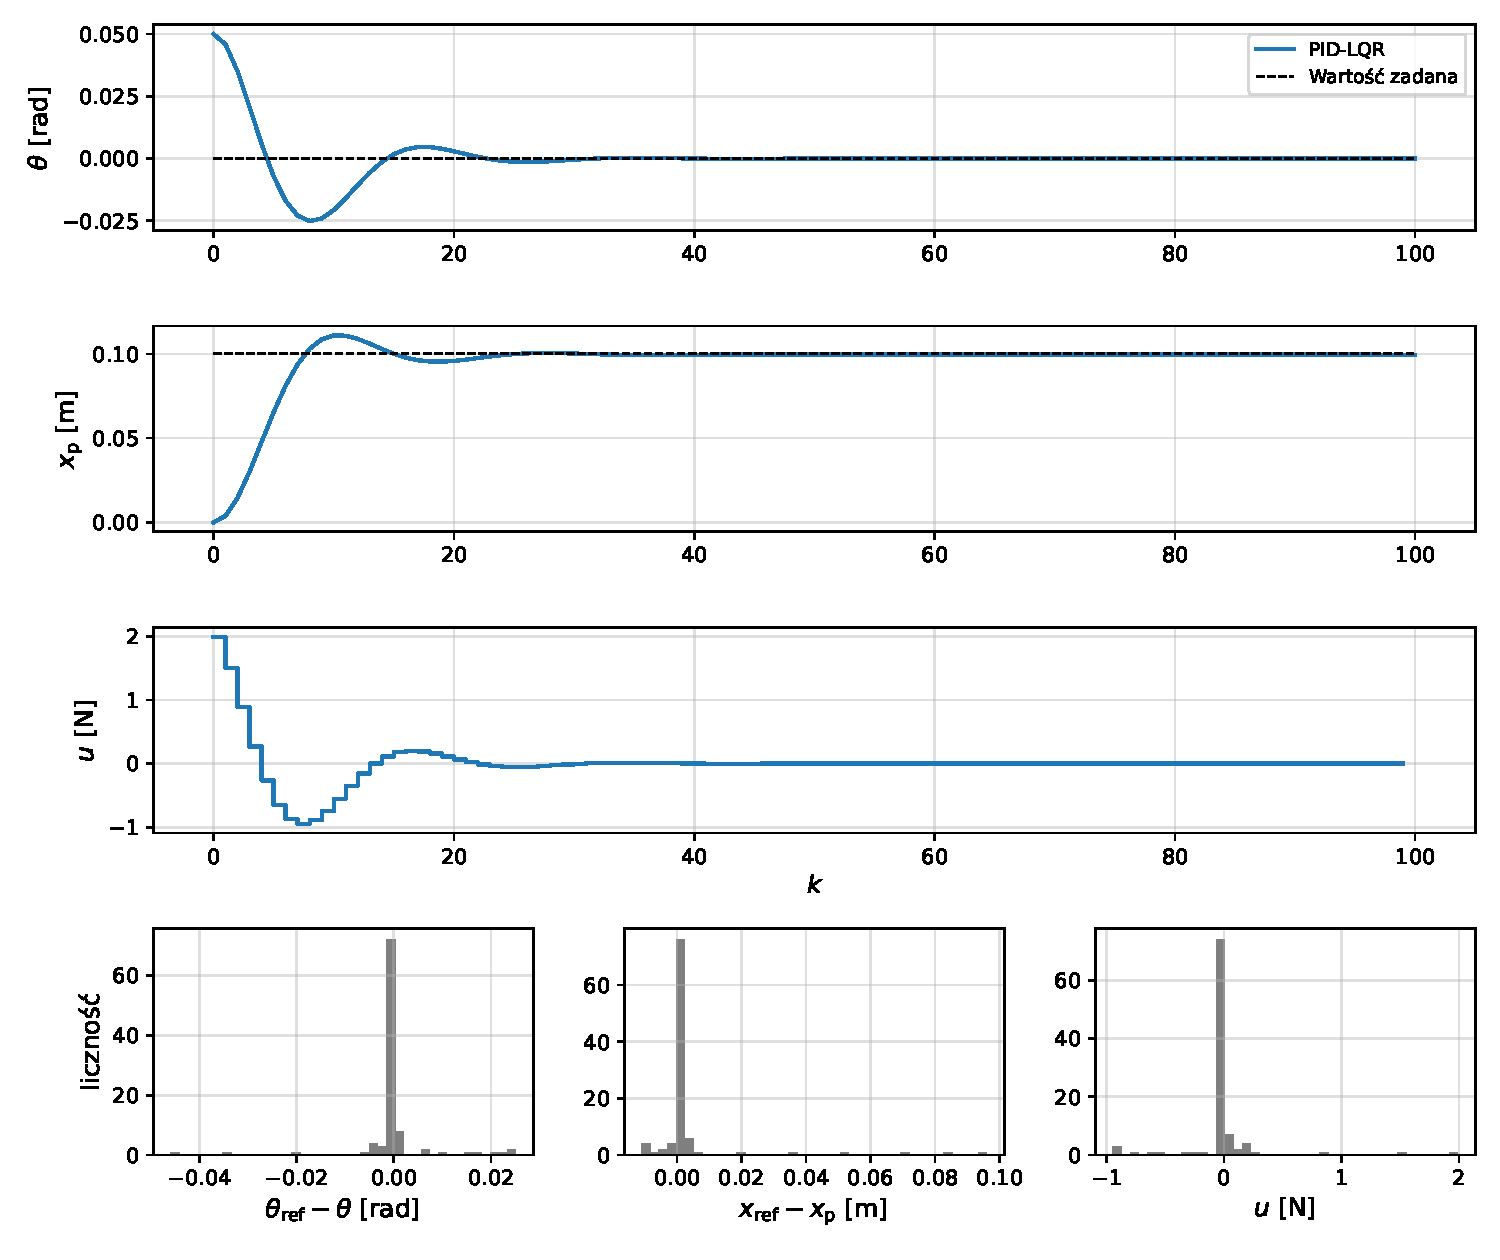
\includegraphics[width=\linewidth]{figs/S1_pid_lqr.pdf}
\caption{PID-LQR, Scenariusz S1 (nominalny): status automatyczny -- stabilny.}
\end{figure}
\clearpage
\begin{figure}[p]\centering
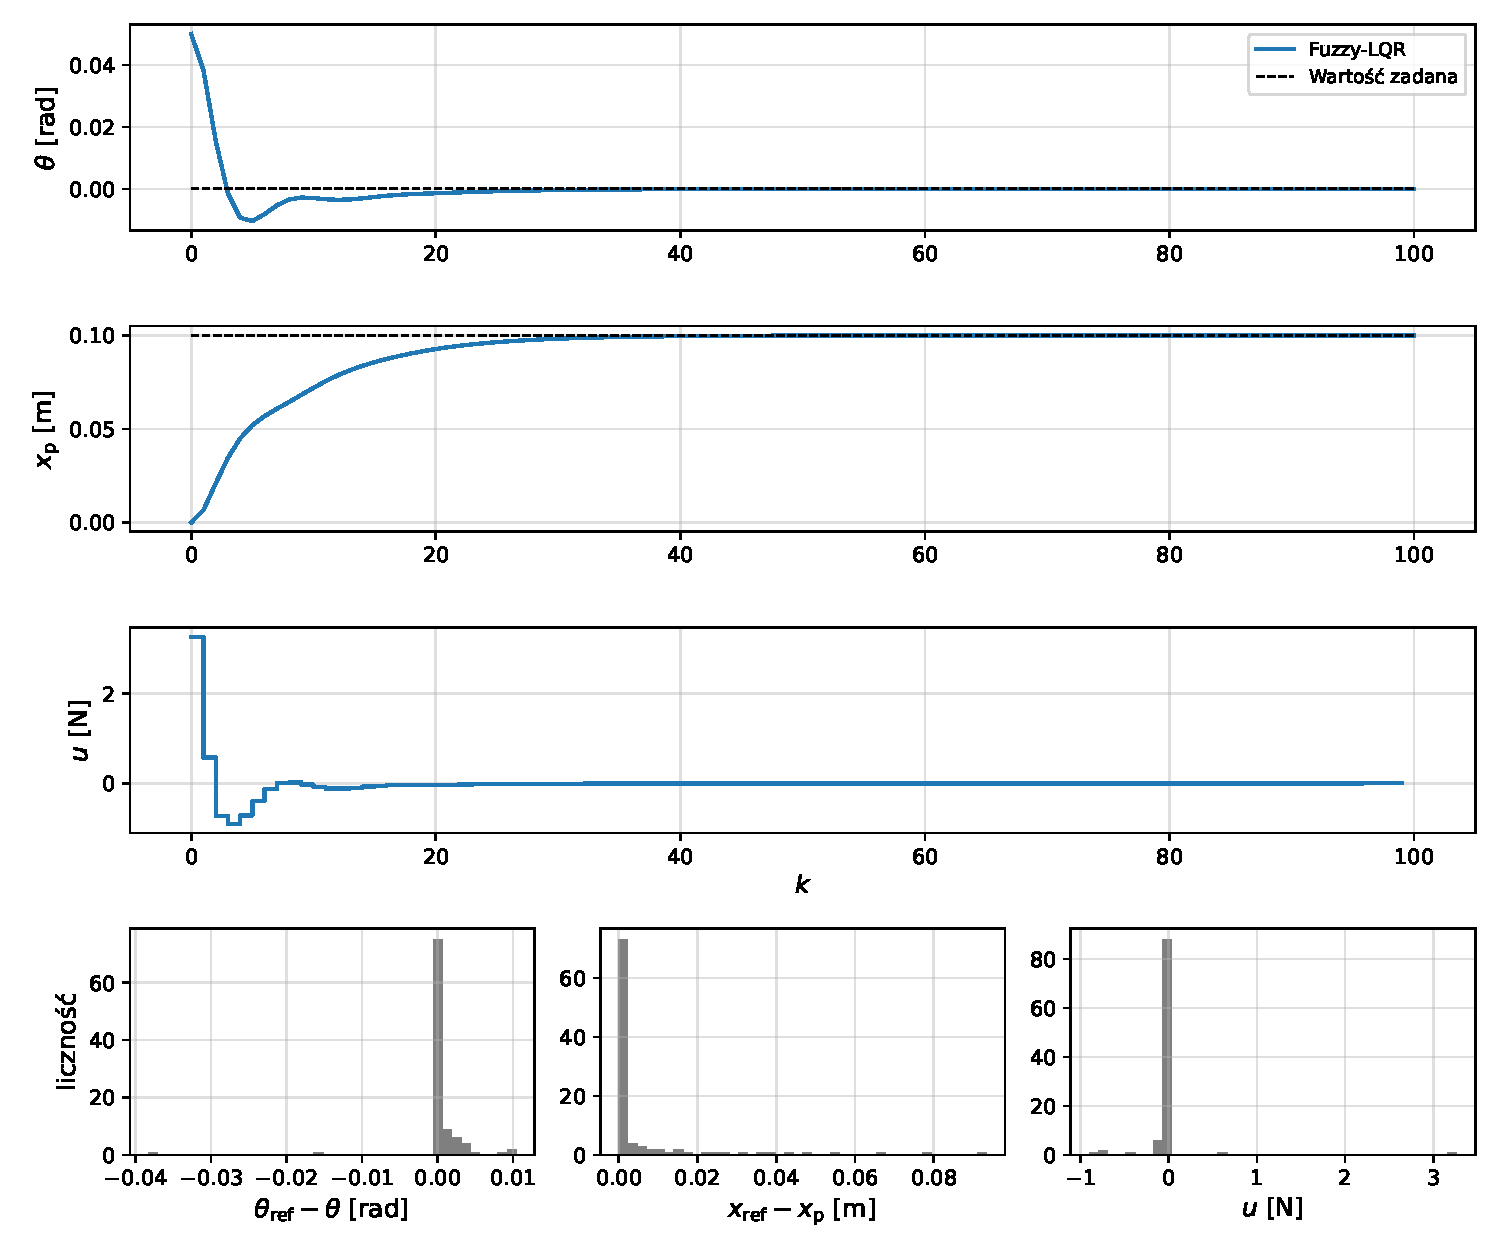
\includegraphics[width=\linewidth]{figs/S1_fuzzy_lqr.pdf}
\caption{Fuzzy-LQR, Scenariusz S1 (nominalny): status automatyczny -- stabilny.}
\end{figure}
\clearpage
\begin{figure}[p]\centering
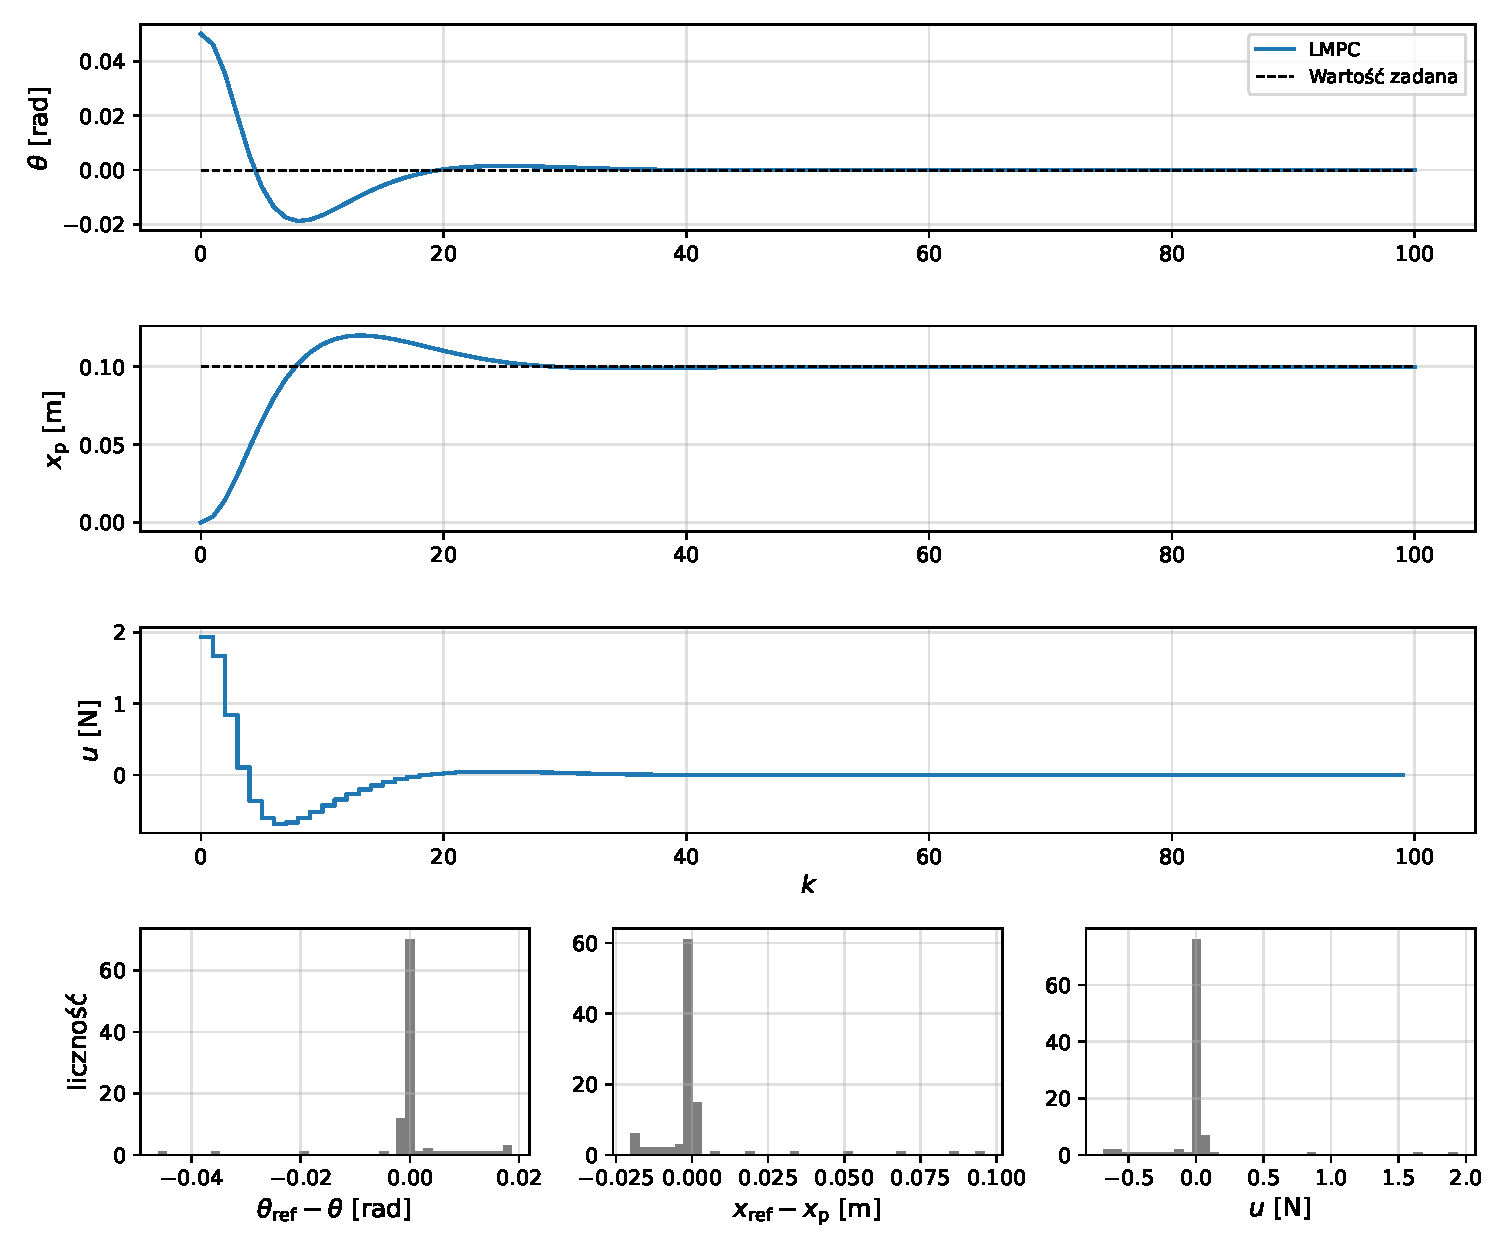
\includegraphics[width=\linewidth]{figs/S1_lmpc.pdf}
\caption{LMPC, Scenariusz S1 (nominalny): status automatyczny -- stabilny.}
\end{figure}
\clearpage
\begin{figure}[p]\centering
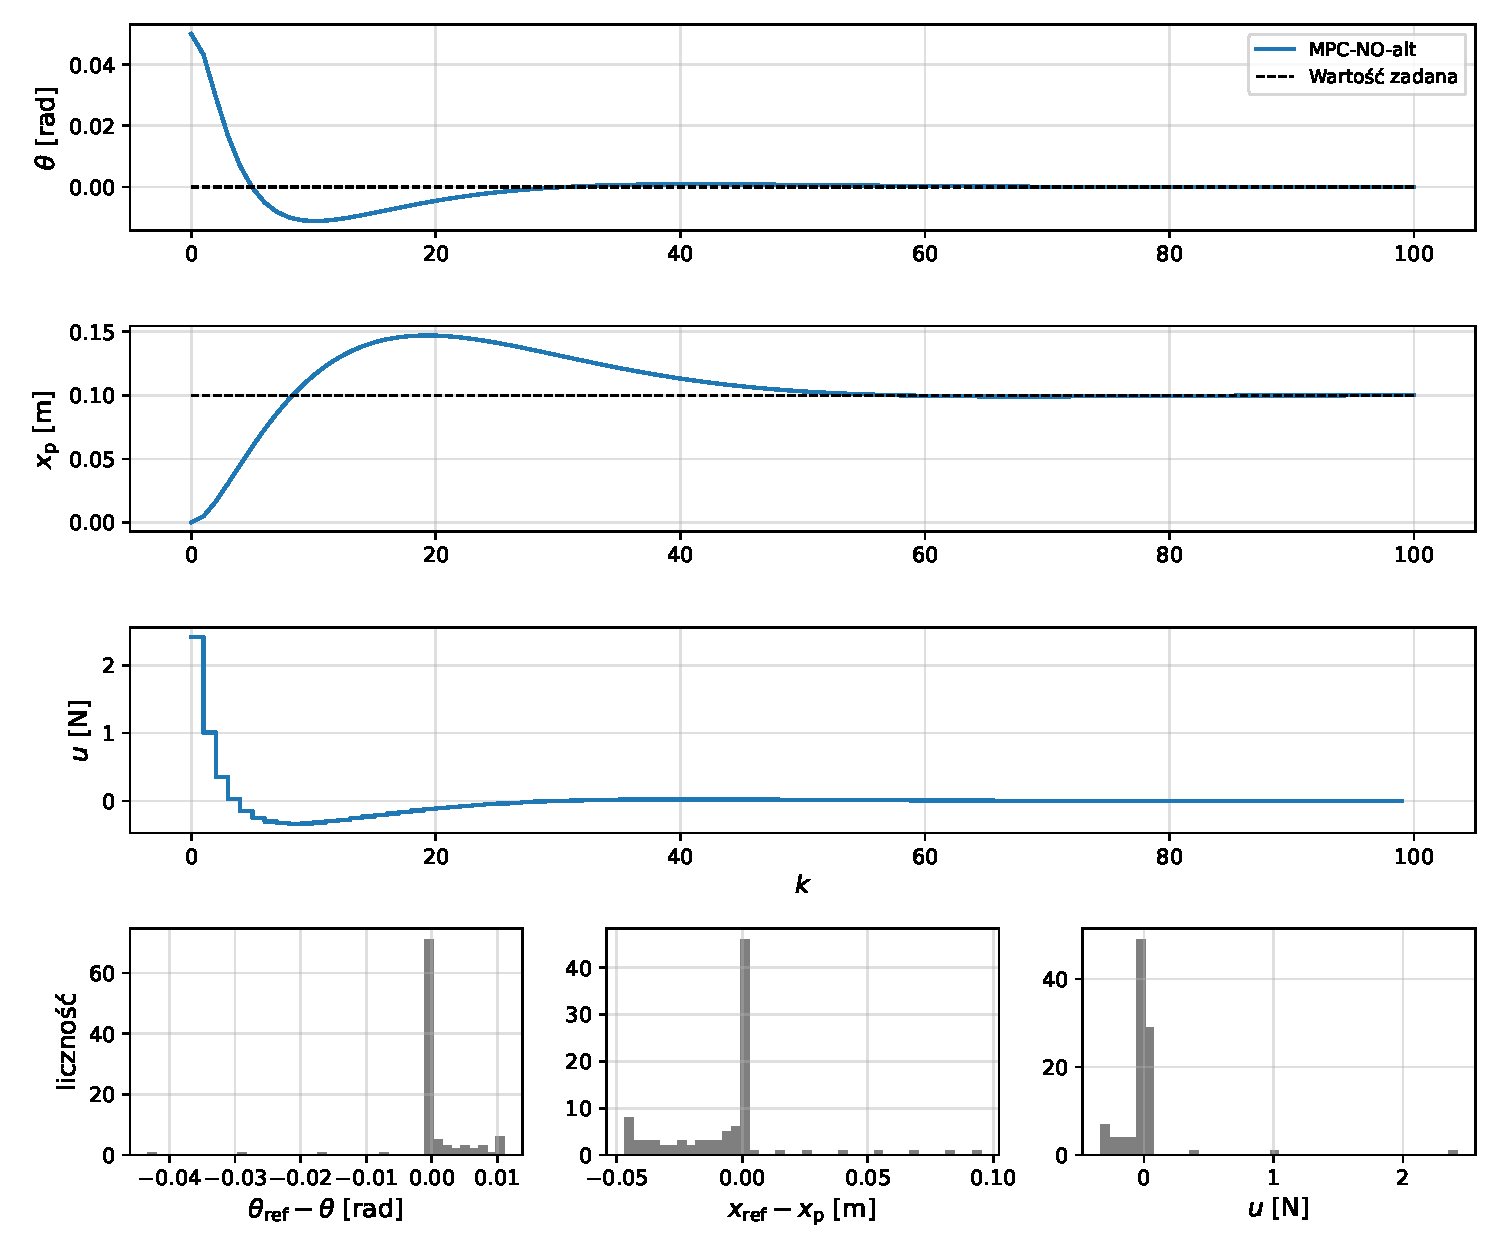
\includegraphics[width=\linewidth]{figs/S1_mpc_no_alt.pdf}
\caption{MPC-NO-alt, Scenariusz S1 (nominalny): status automatyczny -- stabilny.}
\end{figure}
\clearpage
\begin{figure}[p]\centering
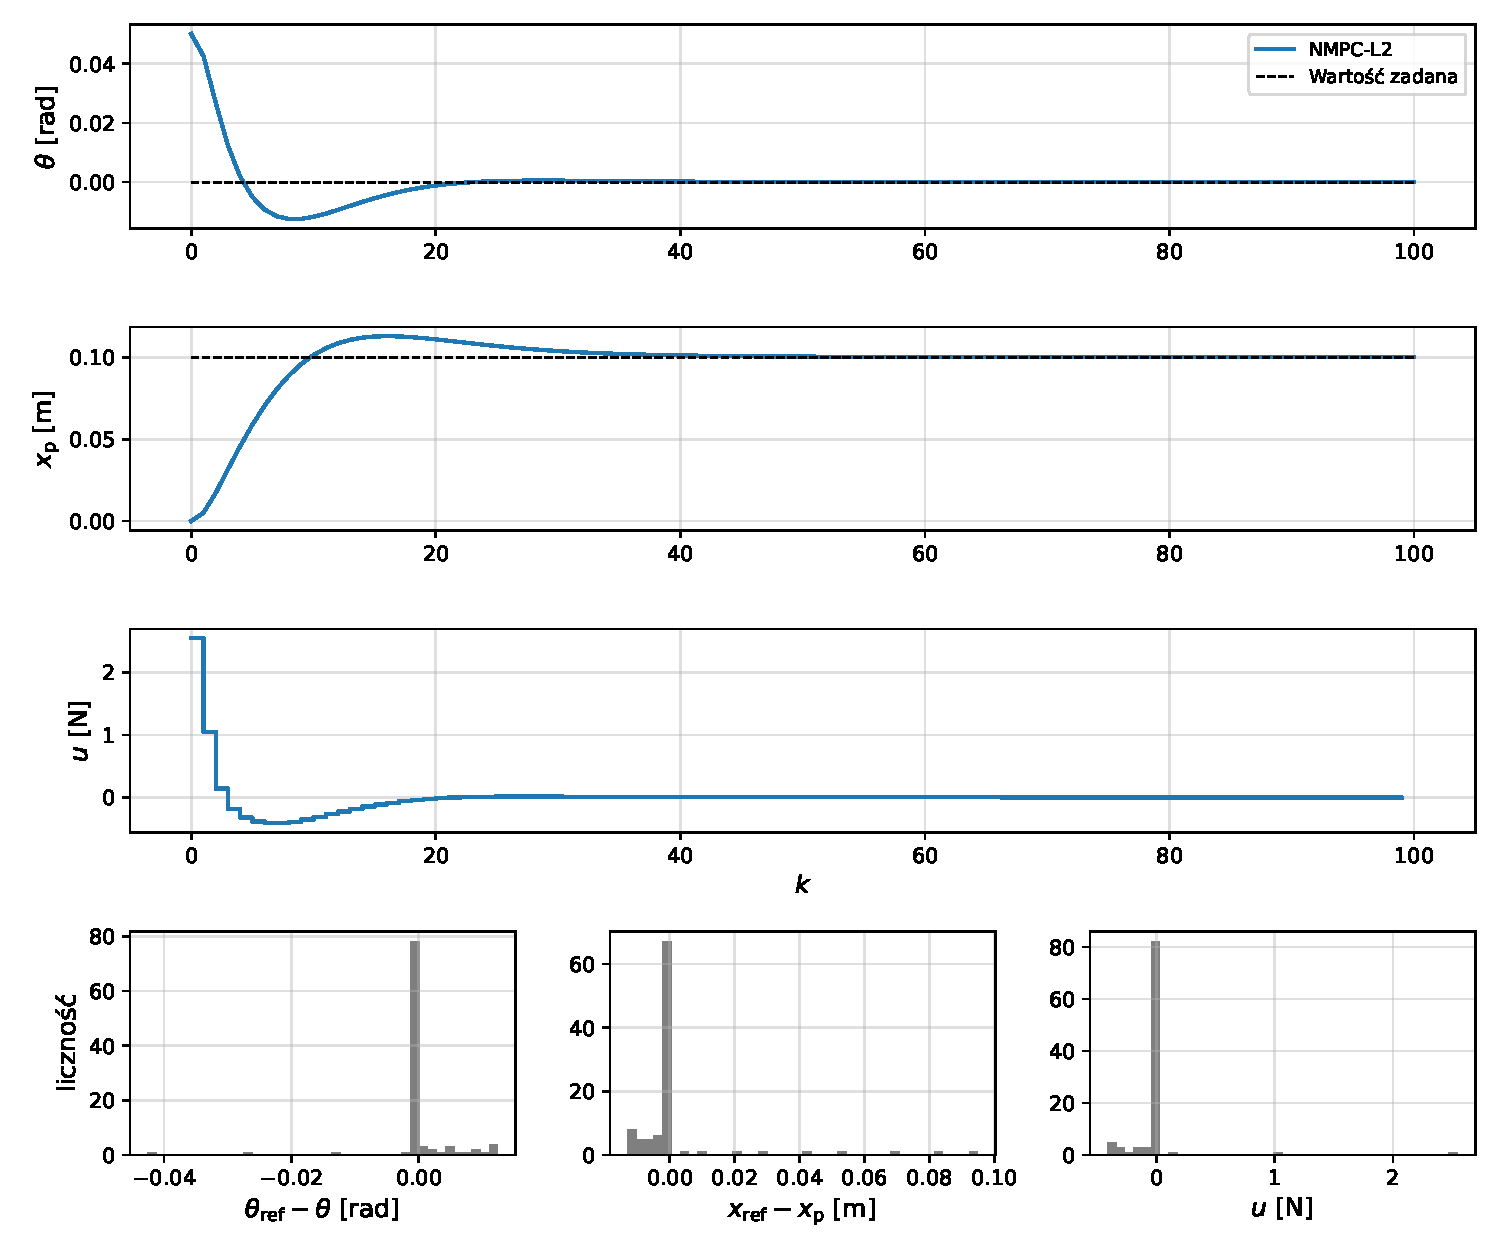
\includegraphics[width=\linewidth]{figs/S1_nmpc_l2.pdf}
\caption{NMPC-L$_2$, Scenariusz S1 (nominalny): status automatyczny -- stabilny.}
\end{figure}
\clearpage
\begin{figure}[p]\centering
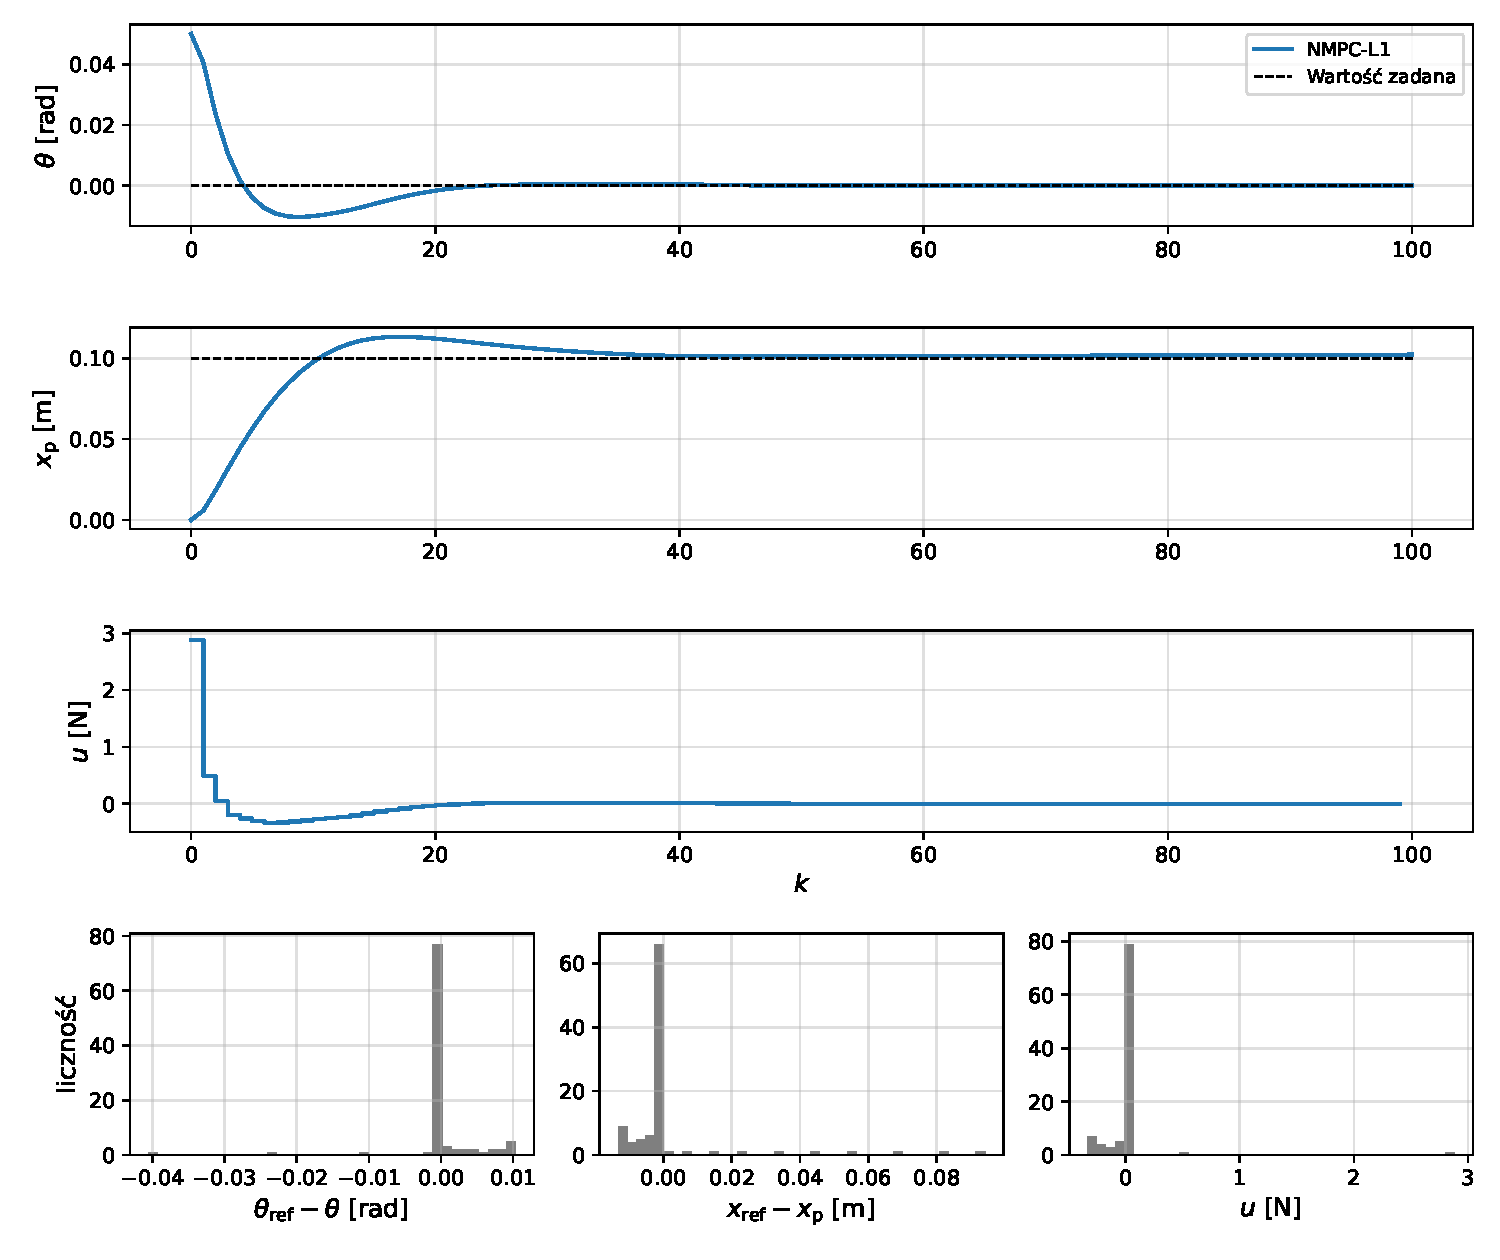
\includegraphics[width=\linewidth]{figs/S1_nmpc_l1.pdf}
\caption{NMPC-L$_1$, Scenariusz S1 (nominalny): status automatyczny -- stabilny.}
\end{figure}
\clearpage
\begin{figure}[p]\centering
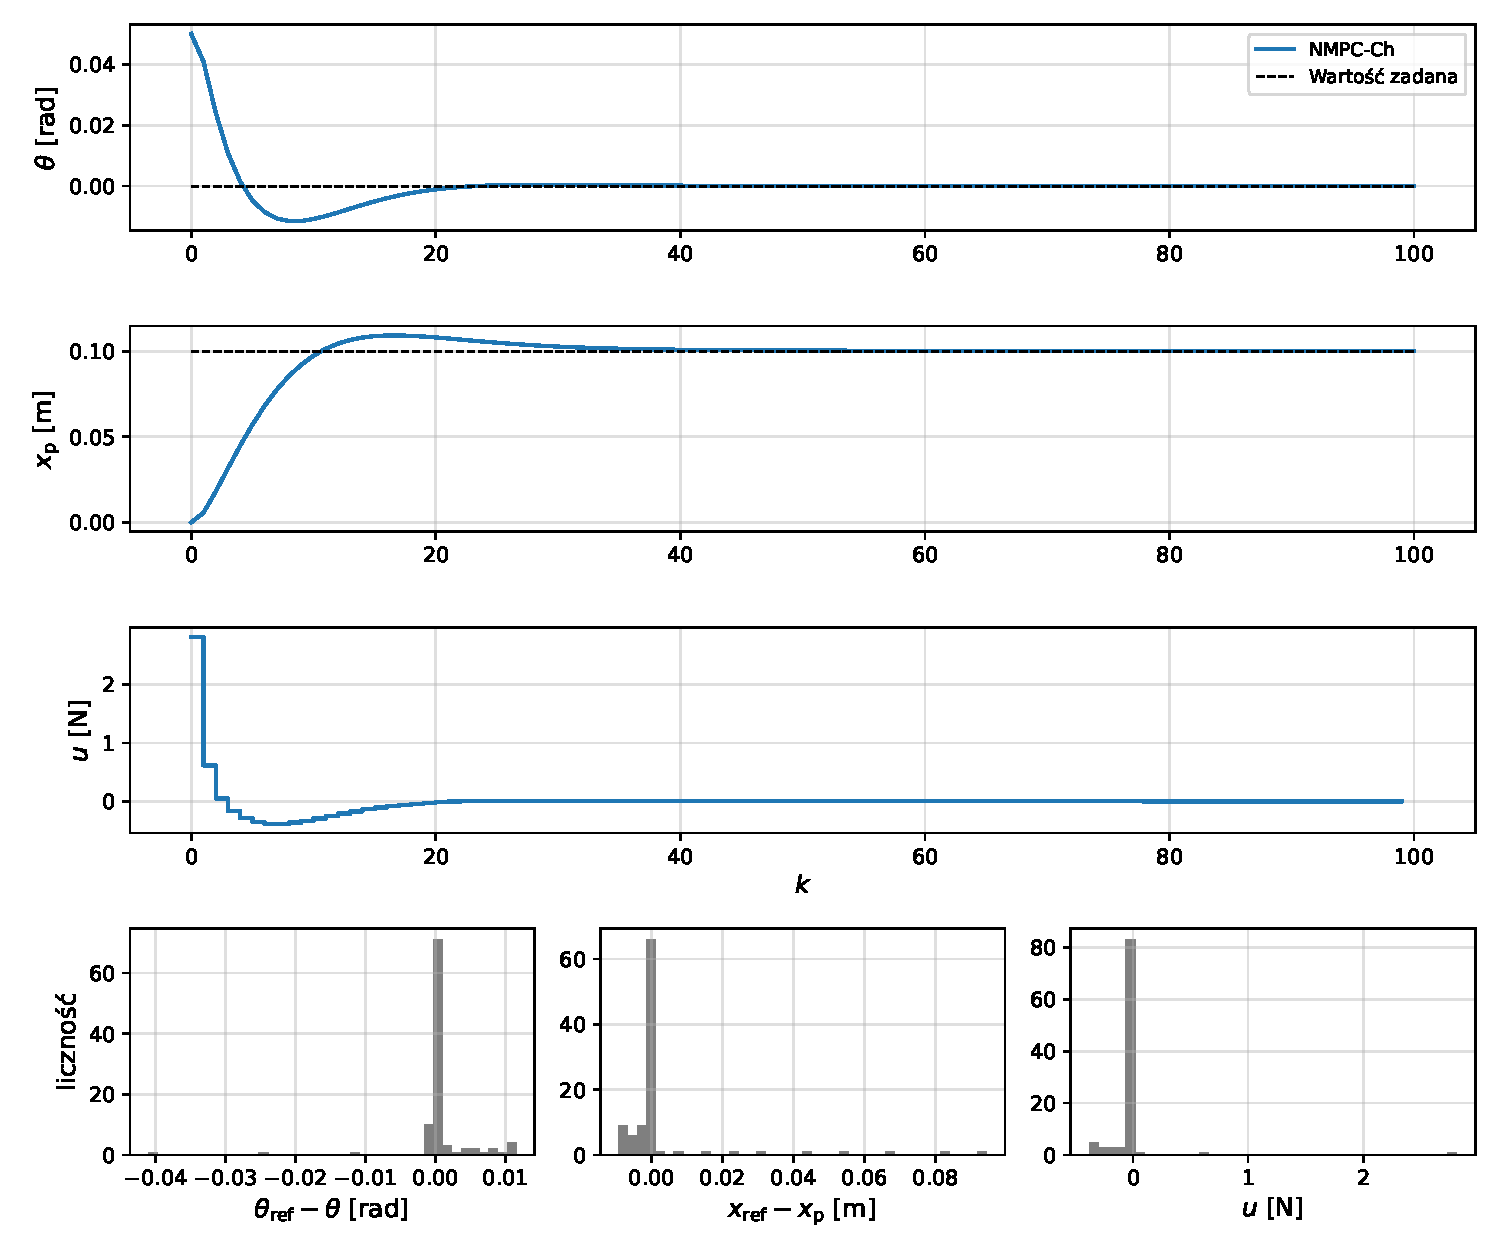
\includegraphics[width=\linewidth]{figs/S1_nmpc_ch.pdf}
\caption{NMPC-Ch, Scenariusz S1 (nominalny): status automatyczny -- stabilny.}
\end{figure}
\clearpage
\begin{figure}[p]\centering
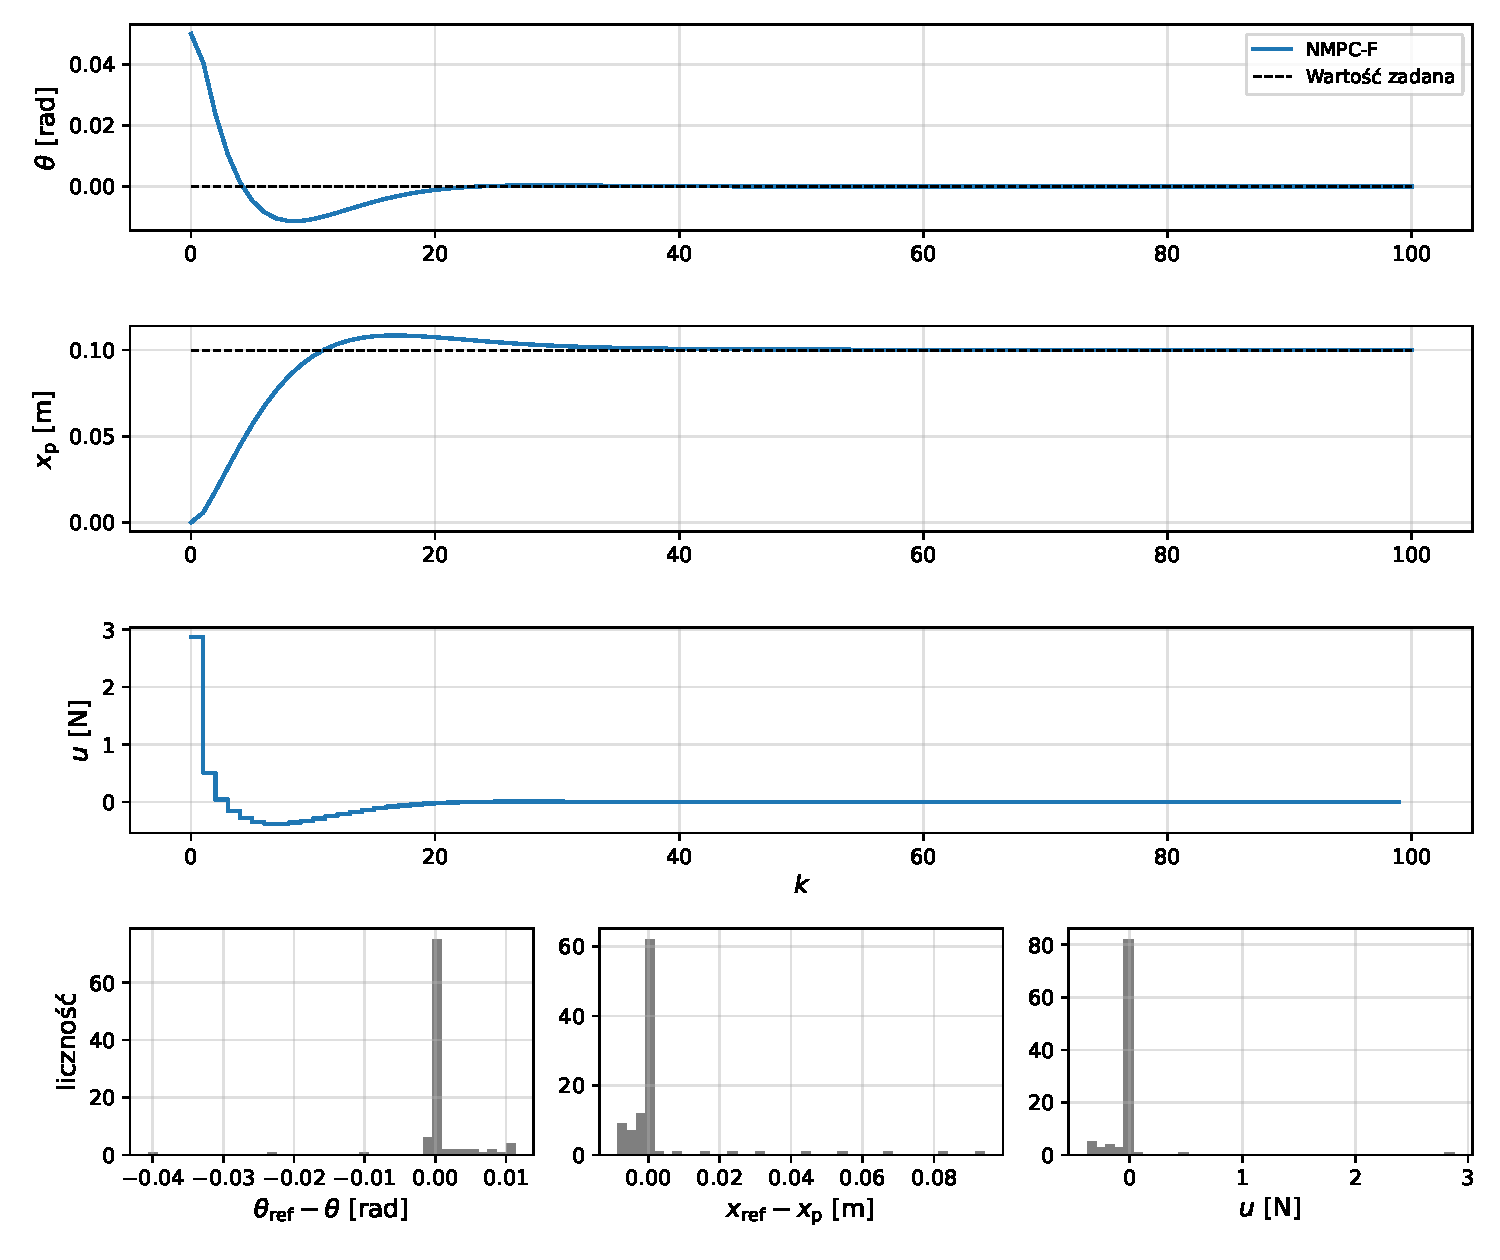
\includegraphics[width=\linewidth]{figs/S1_nmpc_f.pdf}
\caption{NMPC-F, Scenariusz S1 (nominalny): status automatyczny -- stabilny.}
\end{figure}
\clearpage
\begin{figure}[p]\centering
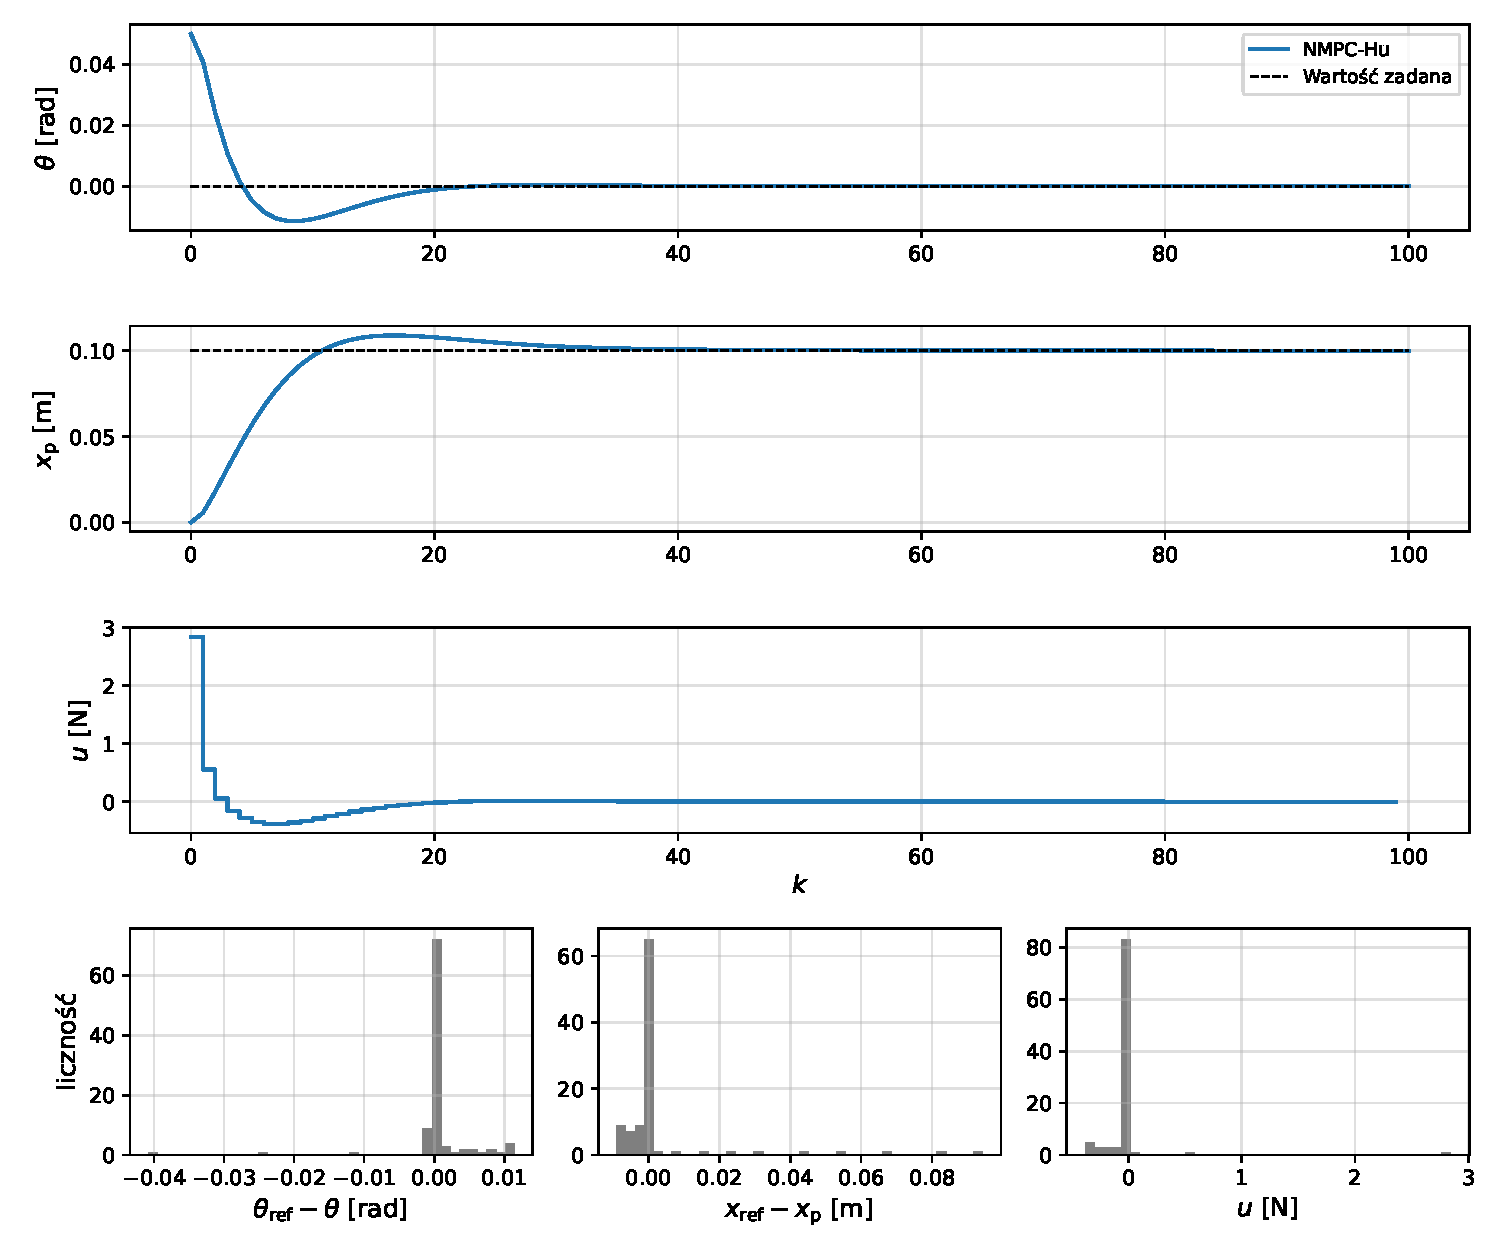
\includegraphics[width=\linewidth]{figs/S1_nmpc_hu.pdf}
\caption{NMPC-Hu, Scenariusz S1 (nominalny): status automatyczny -- stabilny.}
\end{figure}
\clearpage
\begin{figure}[p]\centering
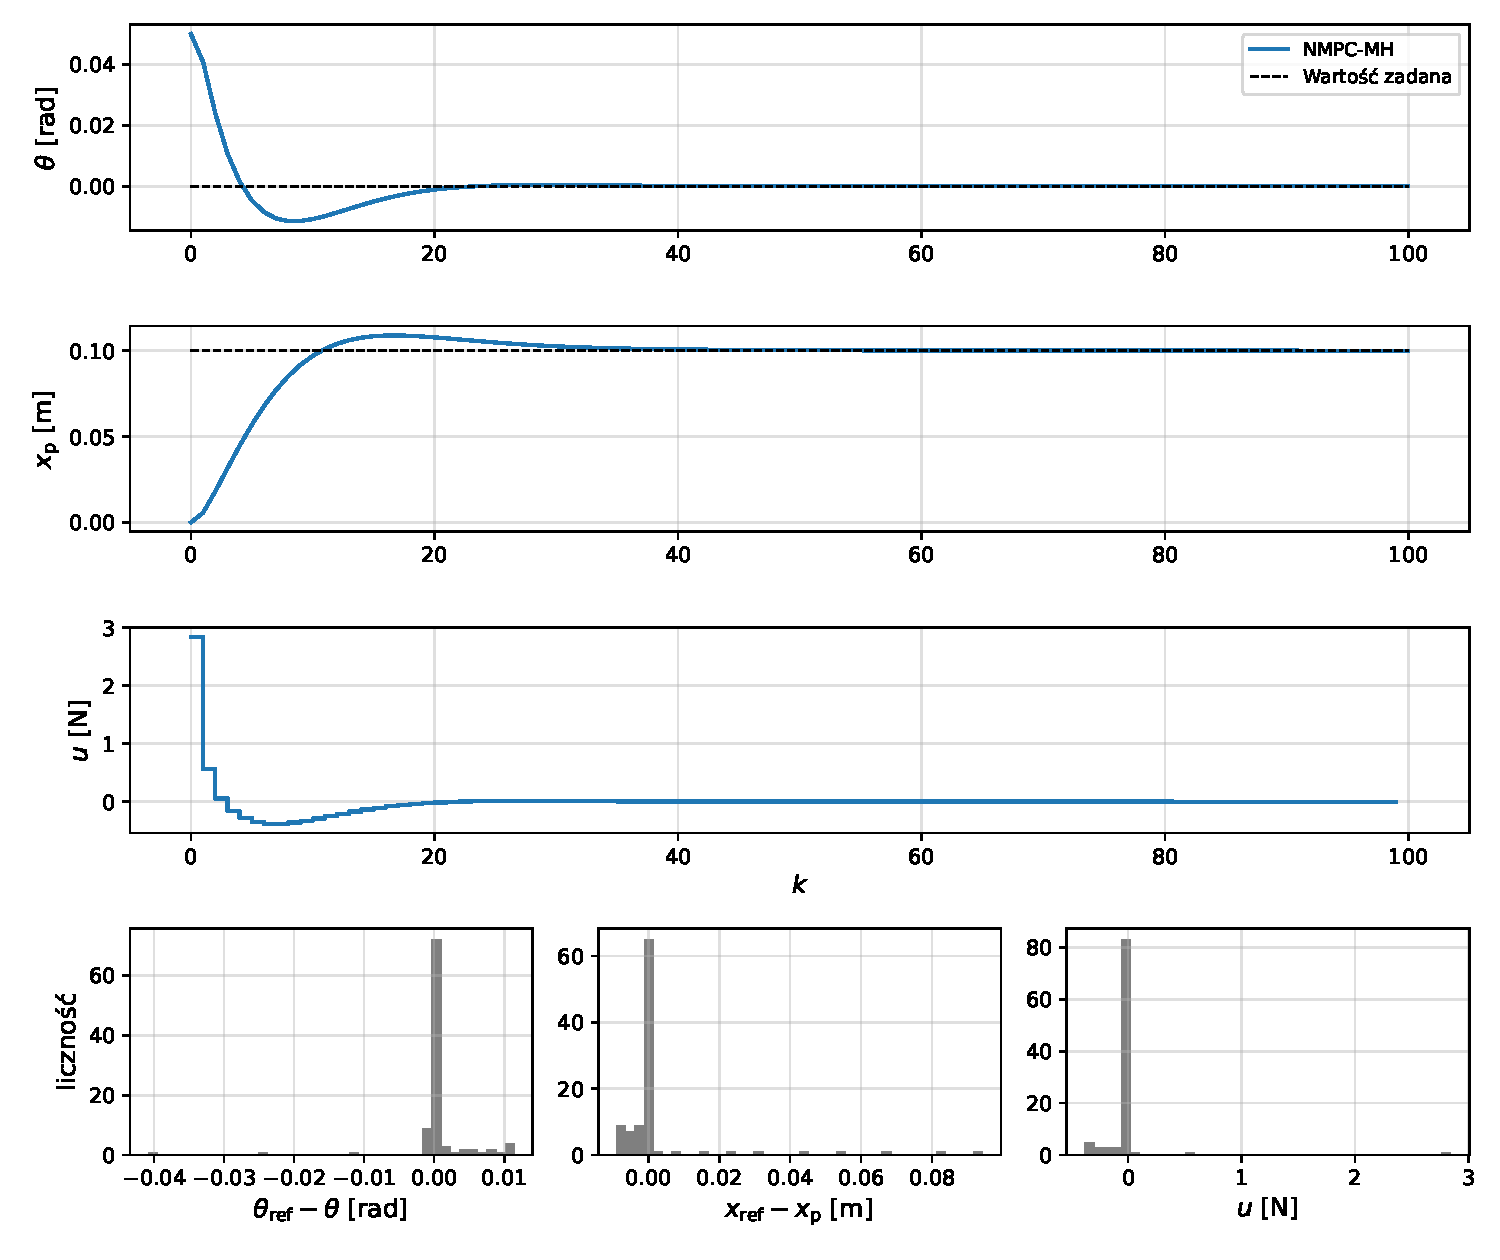
\includegraphics[width=\linewidth]{figs/S1_nmpc_mh.pdf}
\caption{NMPC-MH, Scenariusz S1 (nominalny): status automatyczny -- stabilny.}
\end{figure}
\clearpage
\begin{figure}[p]\centering
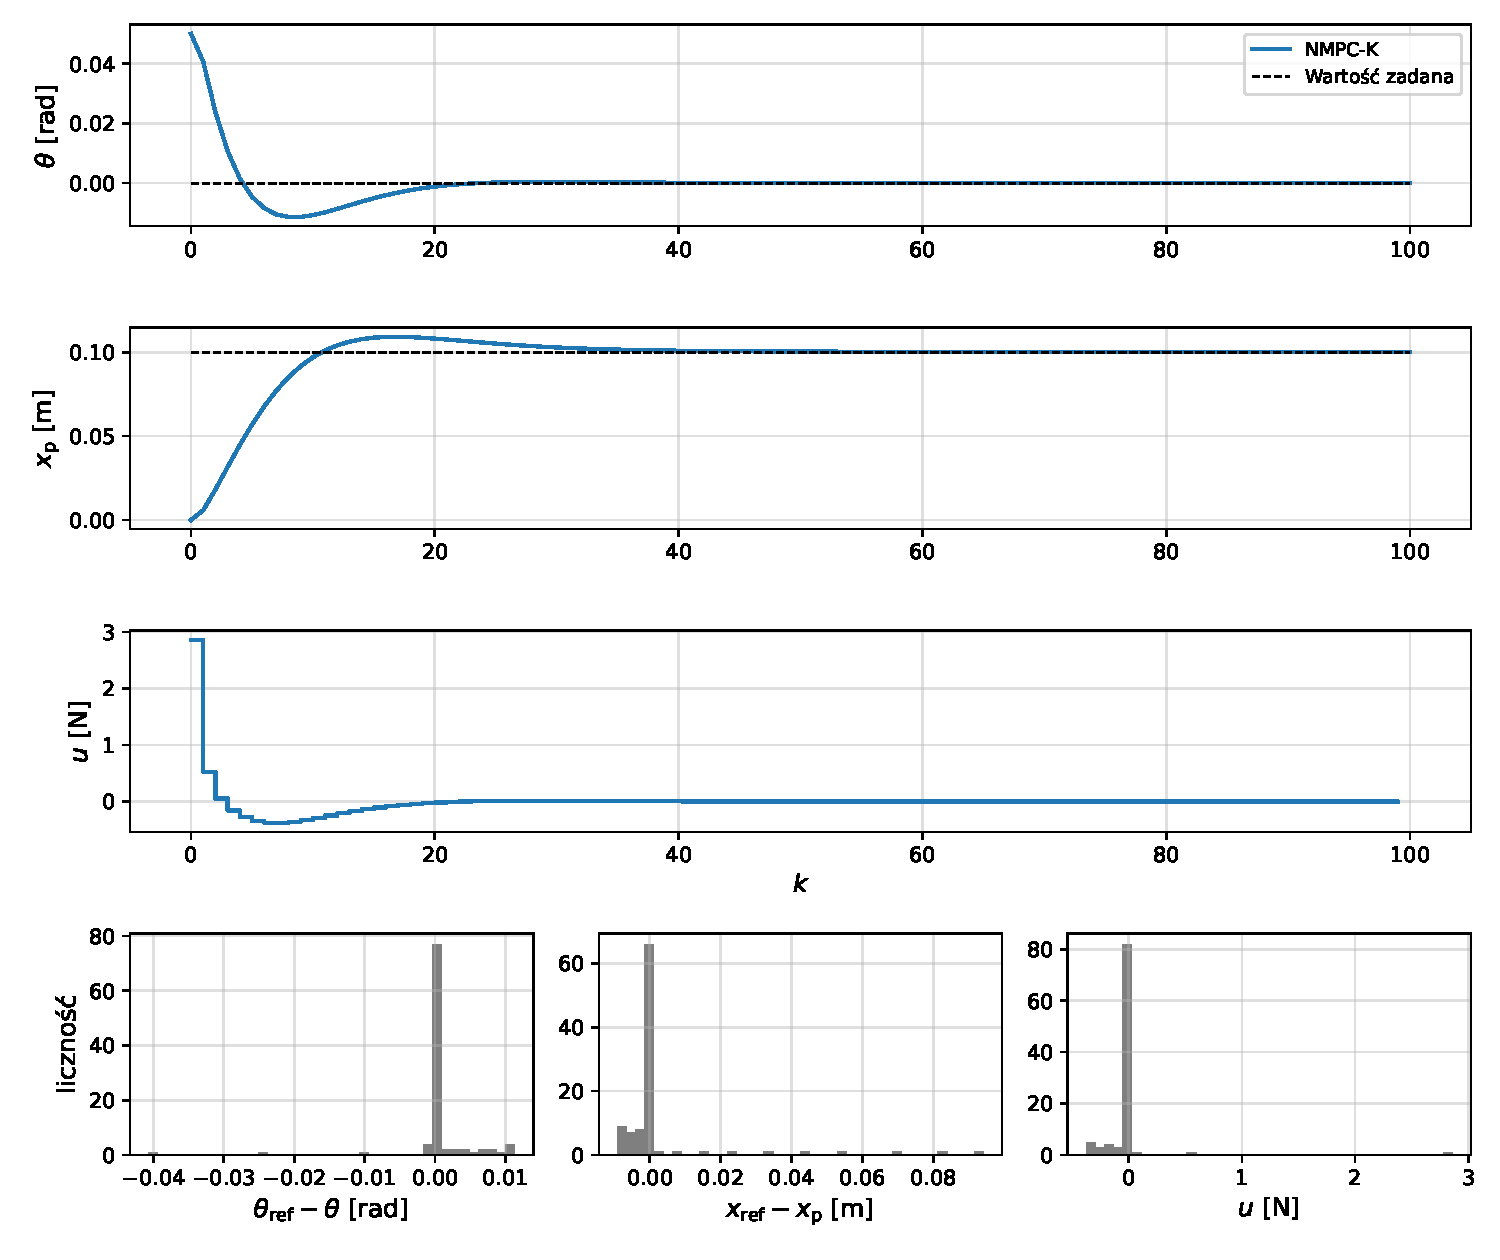
\includegraphics[width=\linewidth]{figs/S1_nmpc_k.pdf}
\caption{NMPC-K, Scenariusz S1 (nominalny): status automatyczny -- stabilny.}
\end{figure}
\clearpage
\begin{figure}[p]\centering
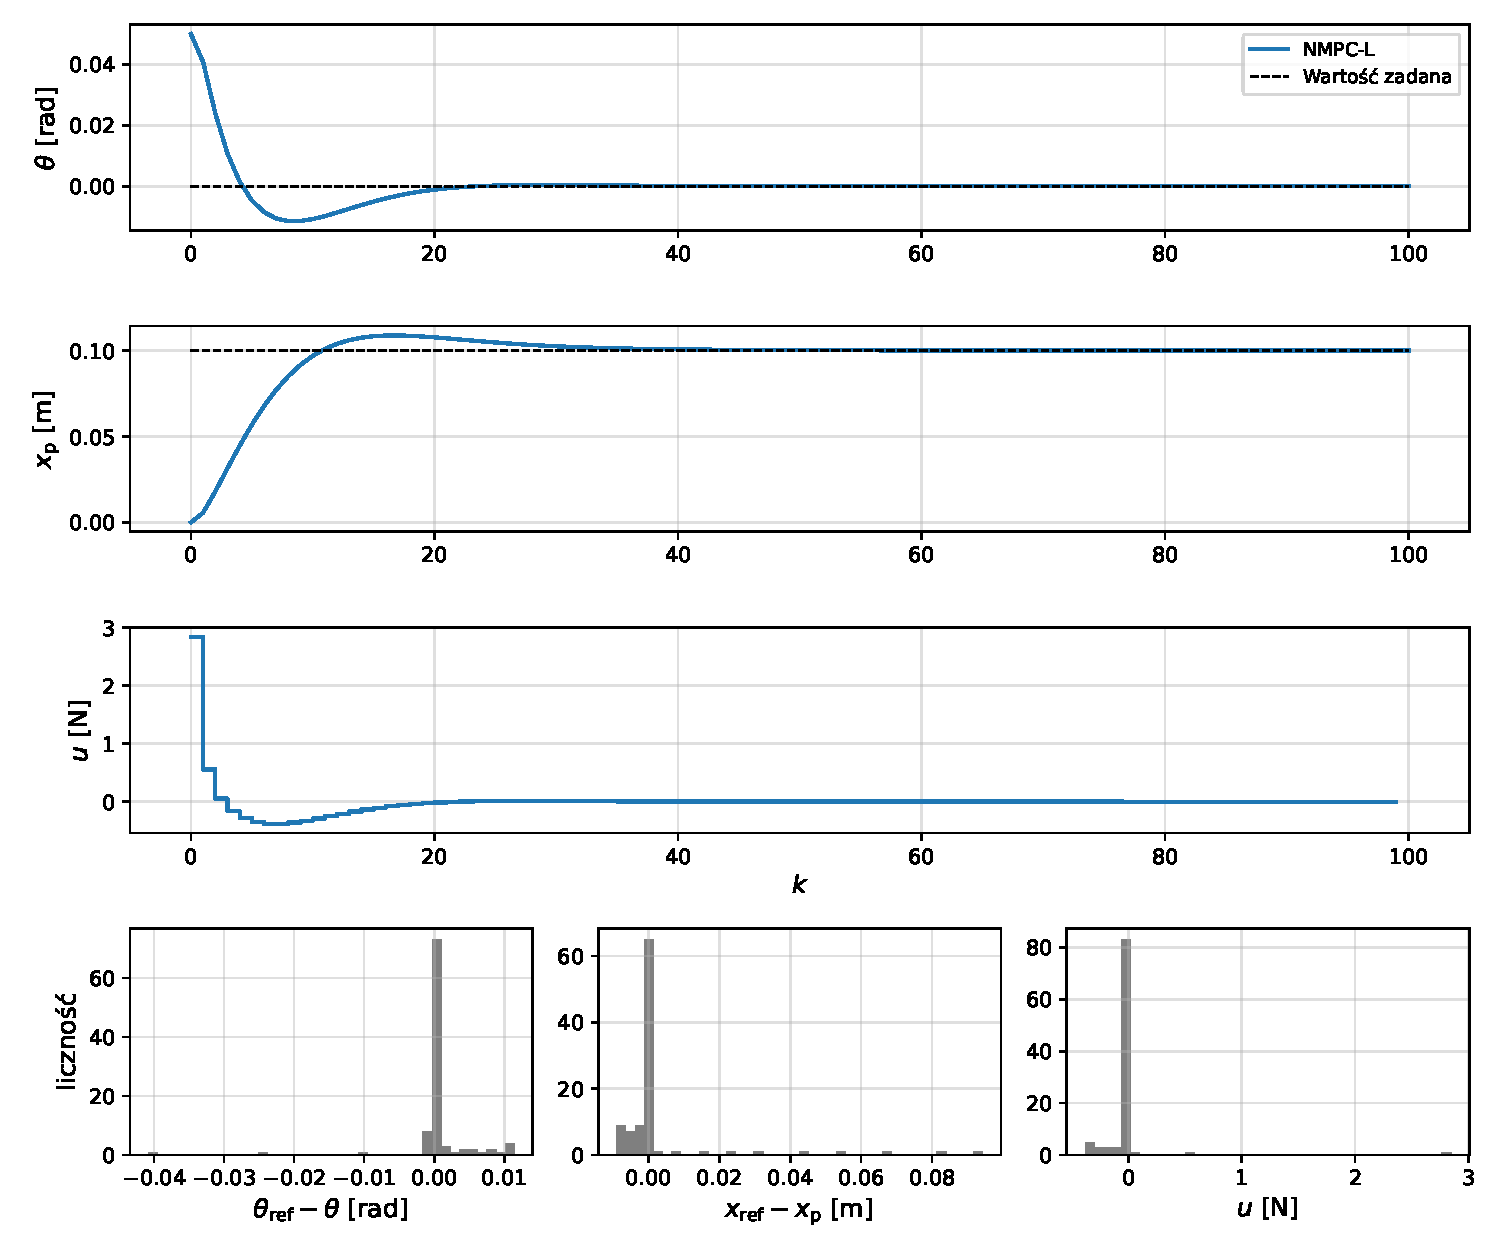
\includegraphics[width=\linewidth]{figs/S1_nmpc_l.pdf}
\caption{NMPC-L, Scenariusz S1 (nominalny): status automatyczny -- stabilny.}
\end{figure}
\clearpage
\begin{figure}[p]\centering
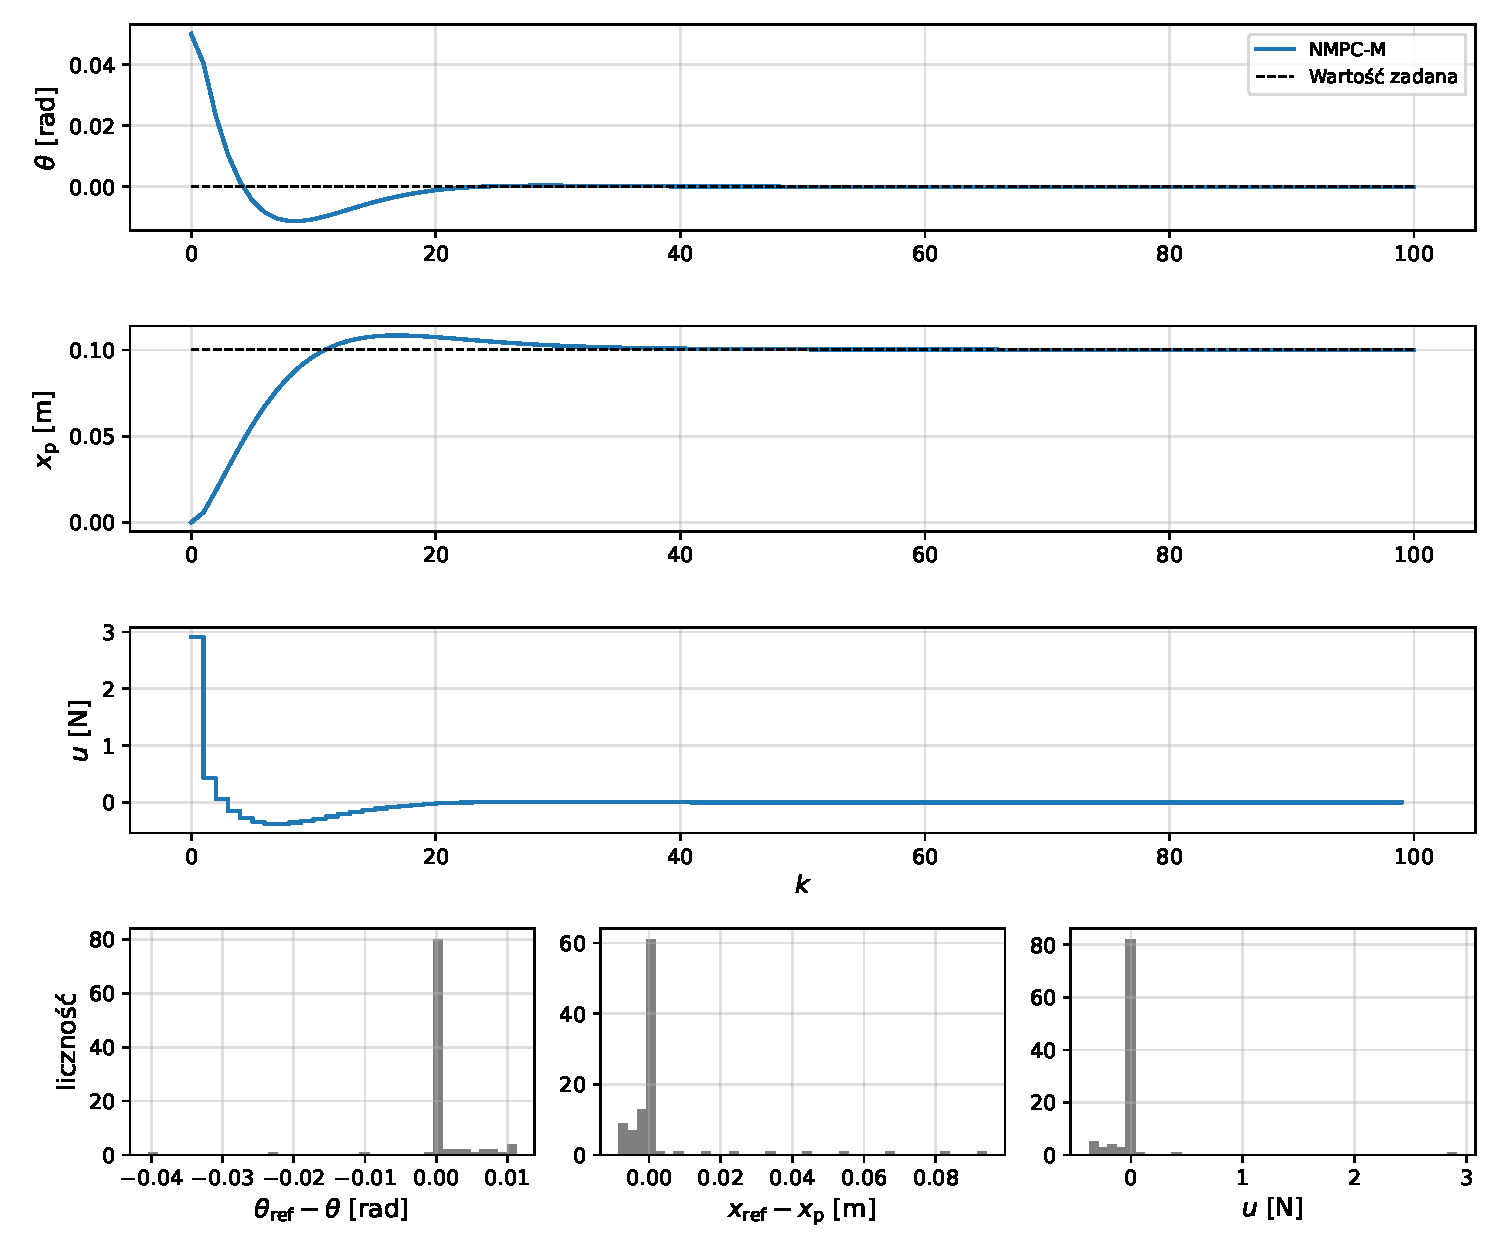
\includegraphics[width=\linewidth]{figs/S1_nmpc_m.pdf}
\caption{NMPC-M, Scenariusz S1 (nominalny): status automatyczny -- stabilny.}
\end{figure}
\clearpage
\begin{figure}[p]\centering
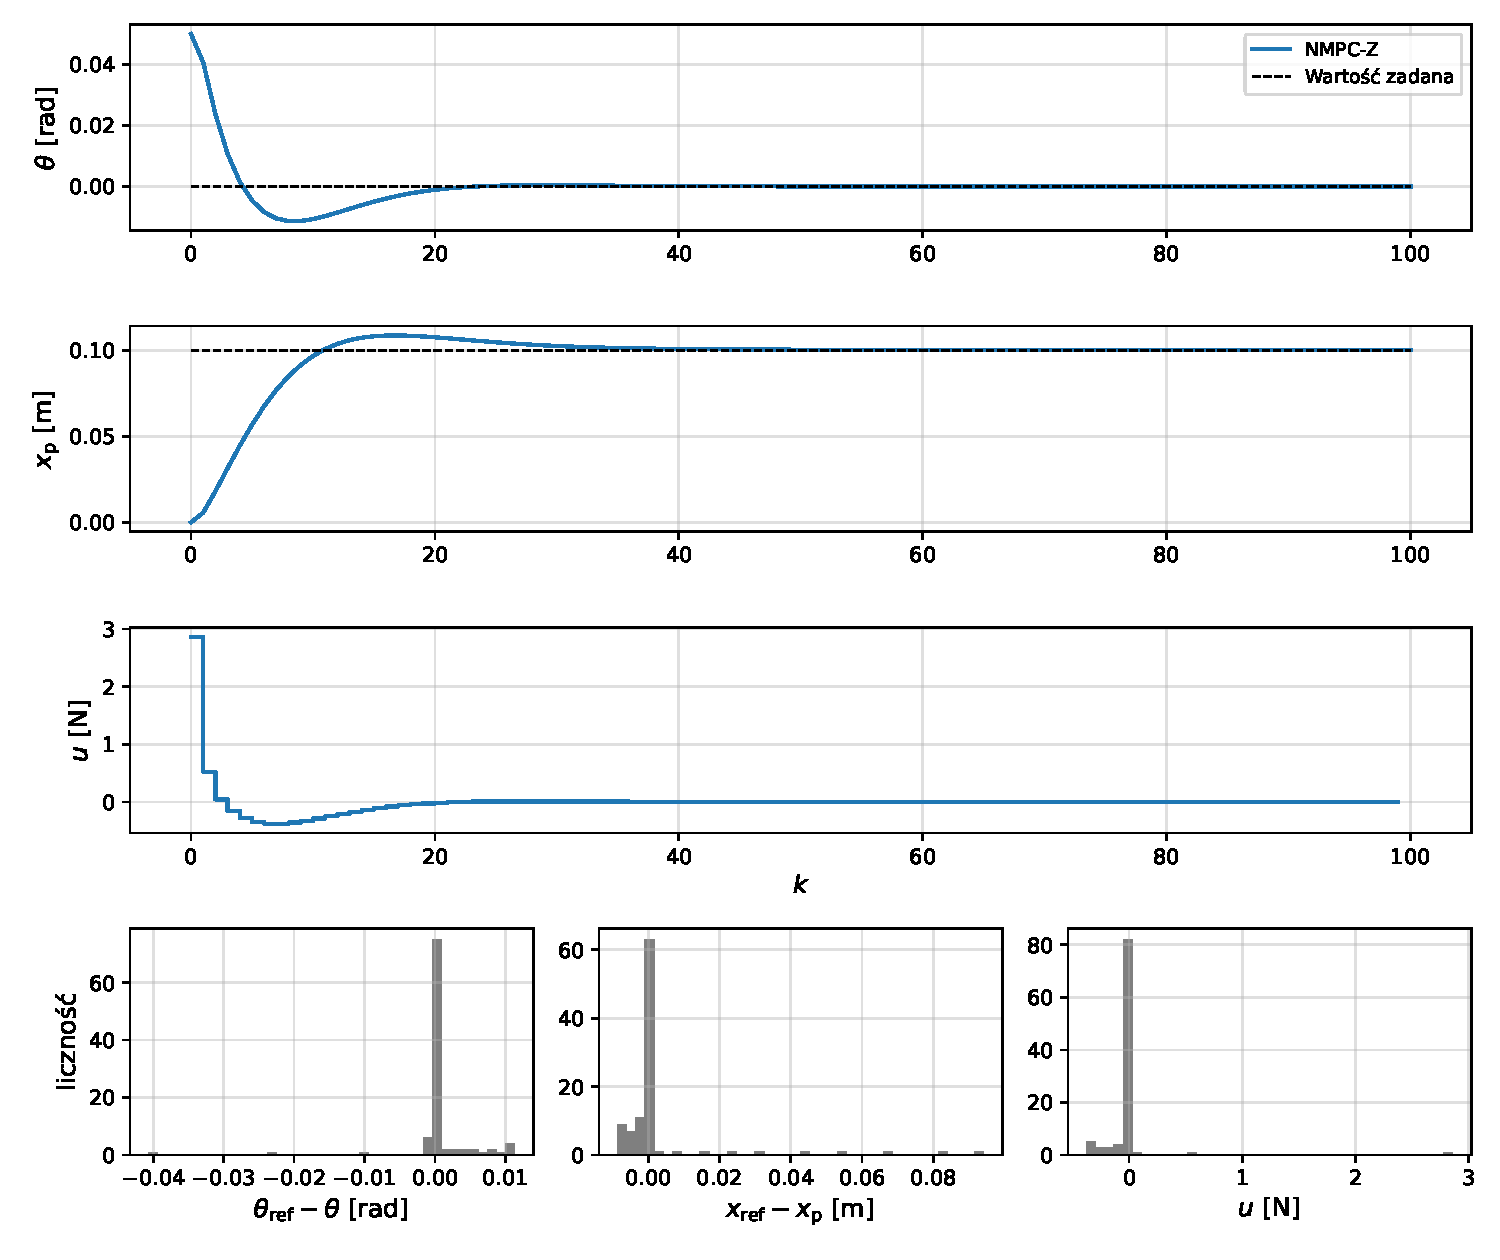
\includegraphics[width=\linewidth]{figs/S1_nmpc_z.pdf}
\caption{NMPC-Z, Scenariusz S1 (nominalny): status automatyczny -- stabilny.}
\end{figure}
\clearpage
\begin{figure}[p]\centering
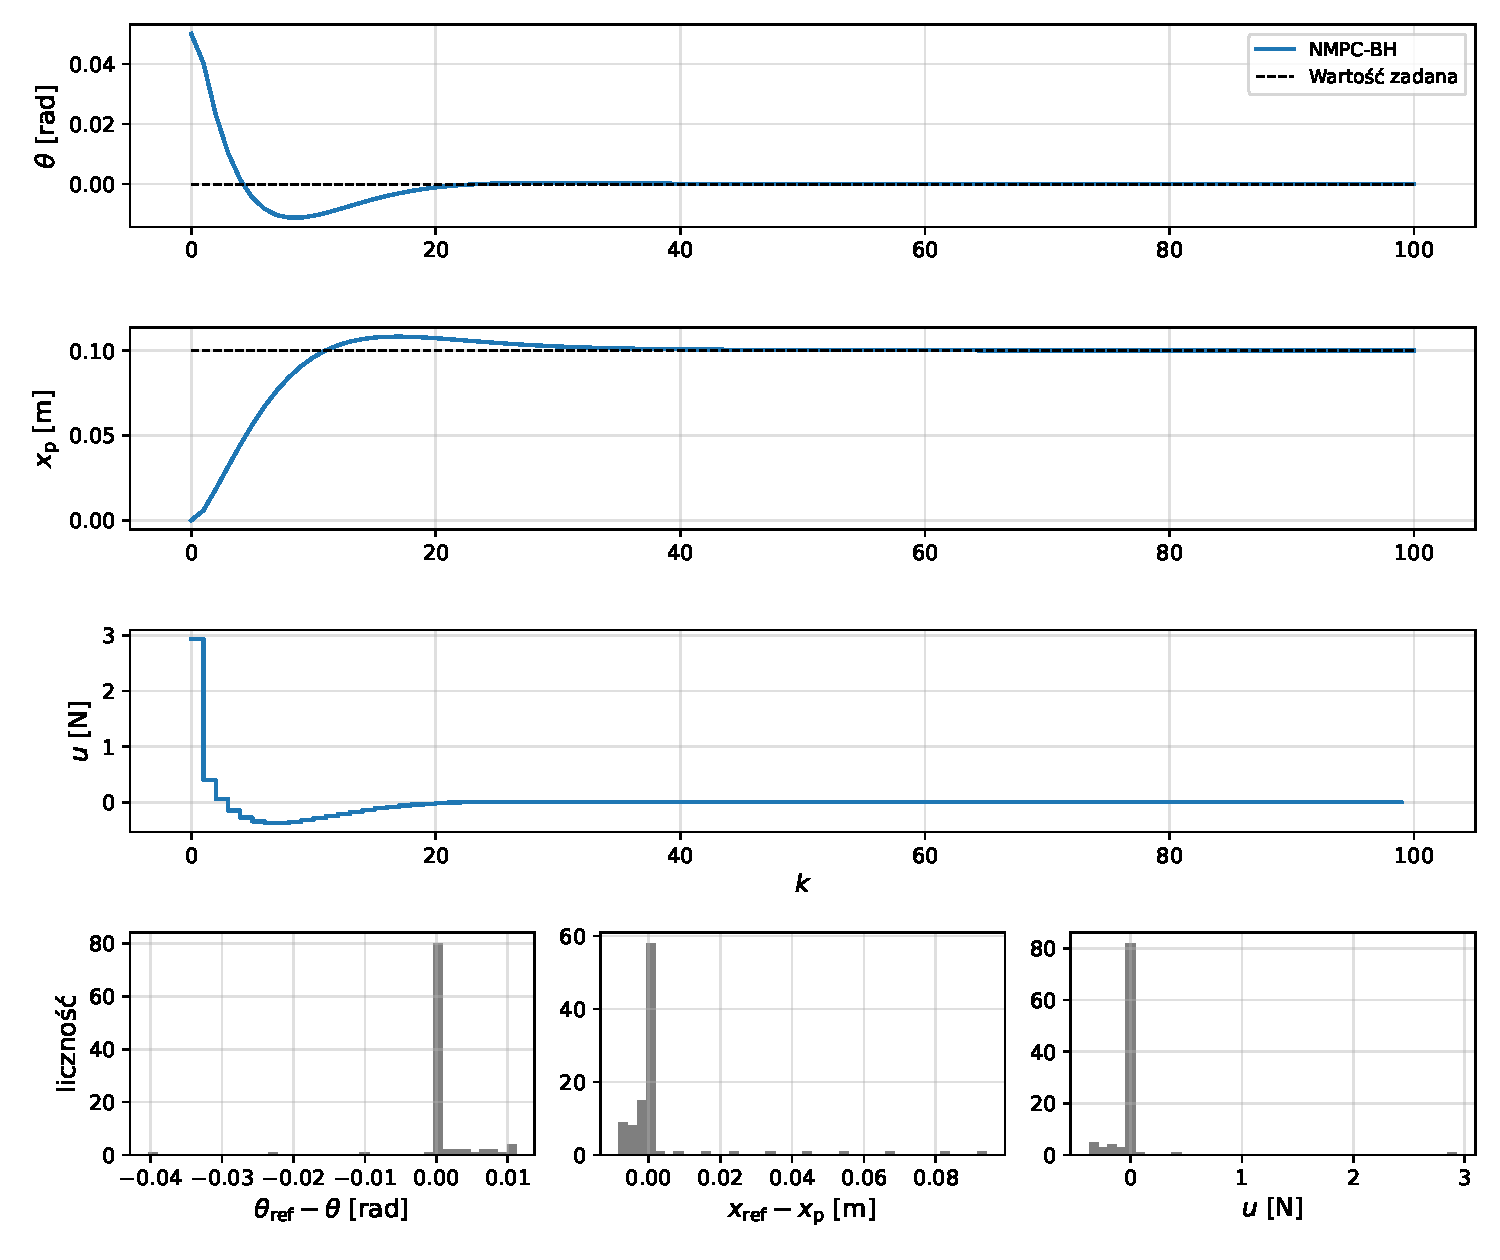
\includegraphics[width=\linewidth]{figs/S1_nmpc_bh.pdf}
\caption{NMPC-BH, Scenariusz S1 (nominalny): status automatyczny -- stabilny.}
\end{figure}
\clearpage
\begin{figure}[p]\centering
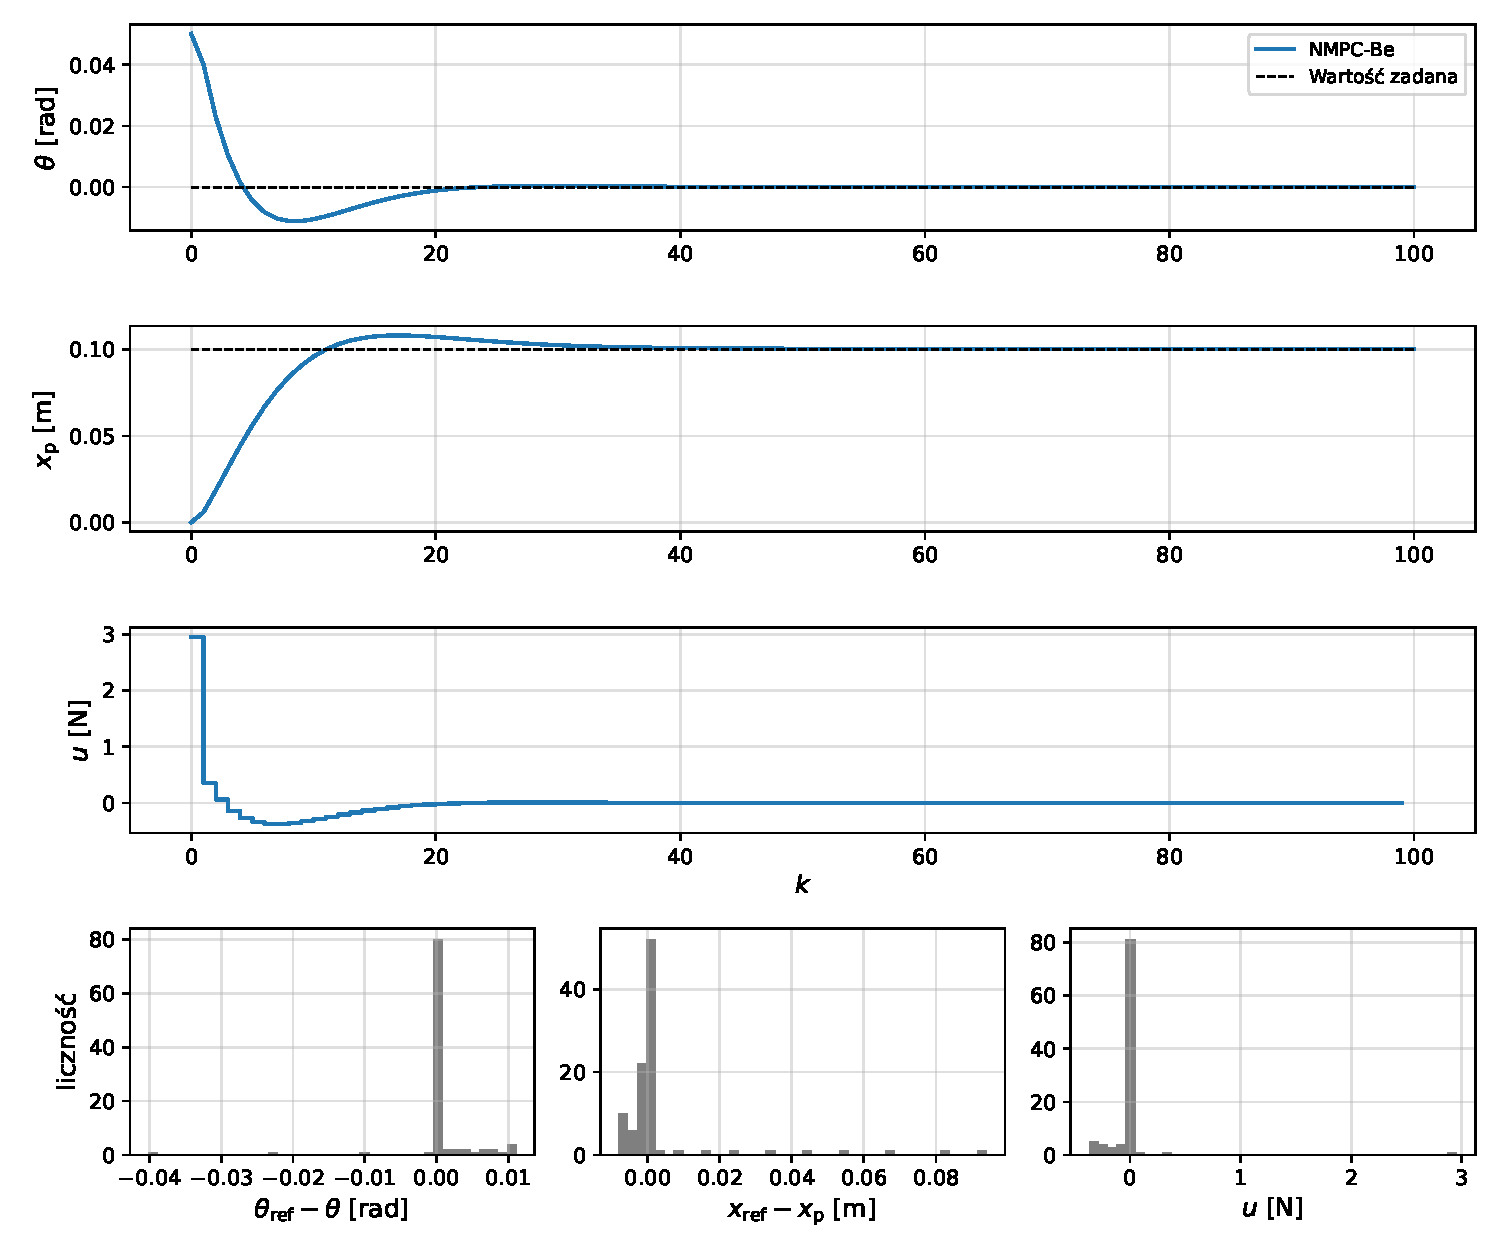
\includegraphics[width=\linewidth]{figs/S1_nmpc_be.pdf}
\caption{NMPC-Be, Scenariusz S1 (nominalny): status automatyczny -- stabilny.}
\end{figure}
\clearpage
\begin{figure}[p]\centering
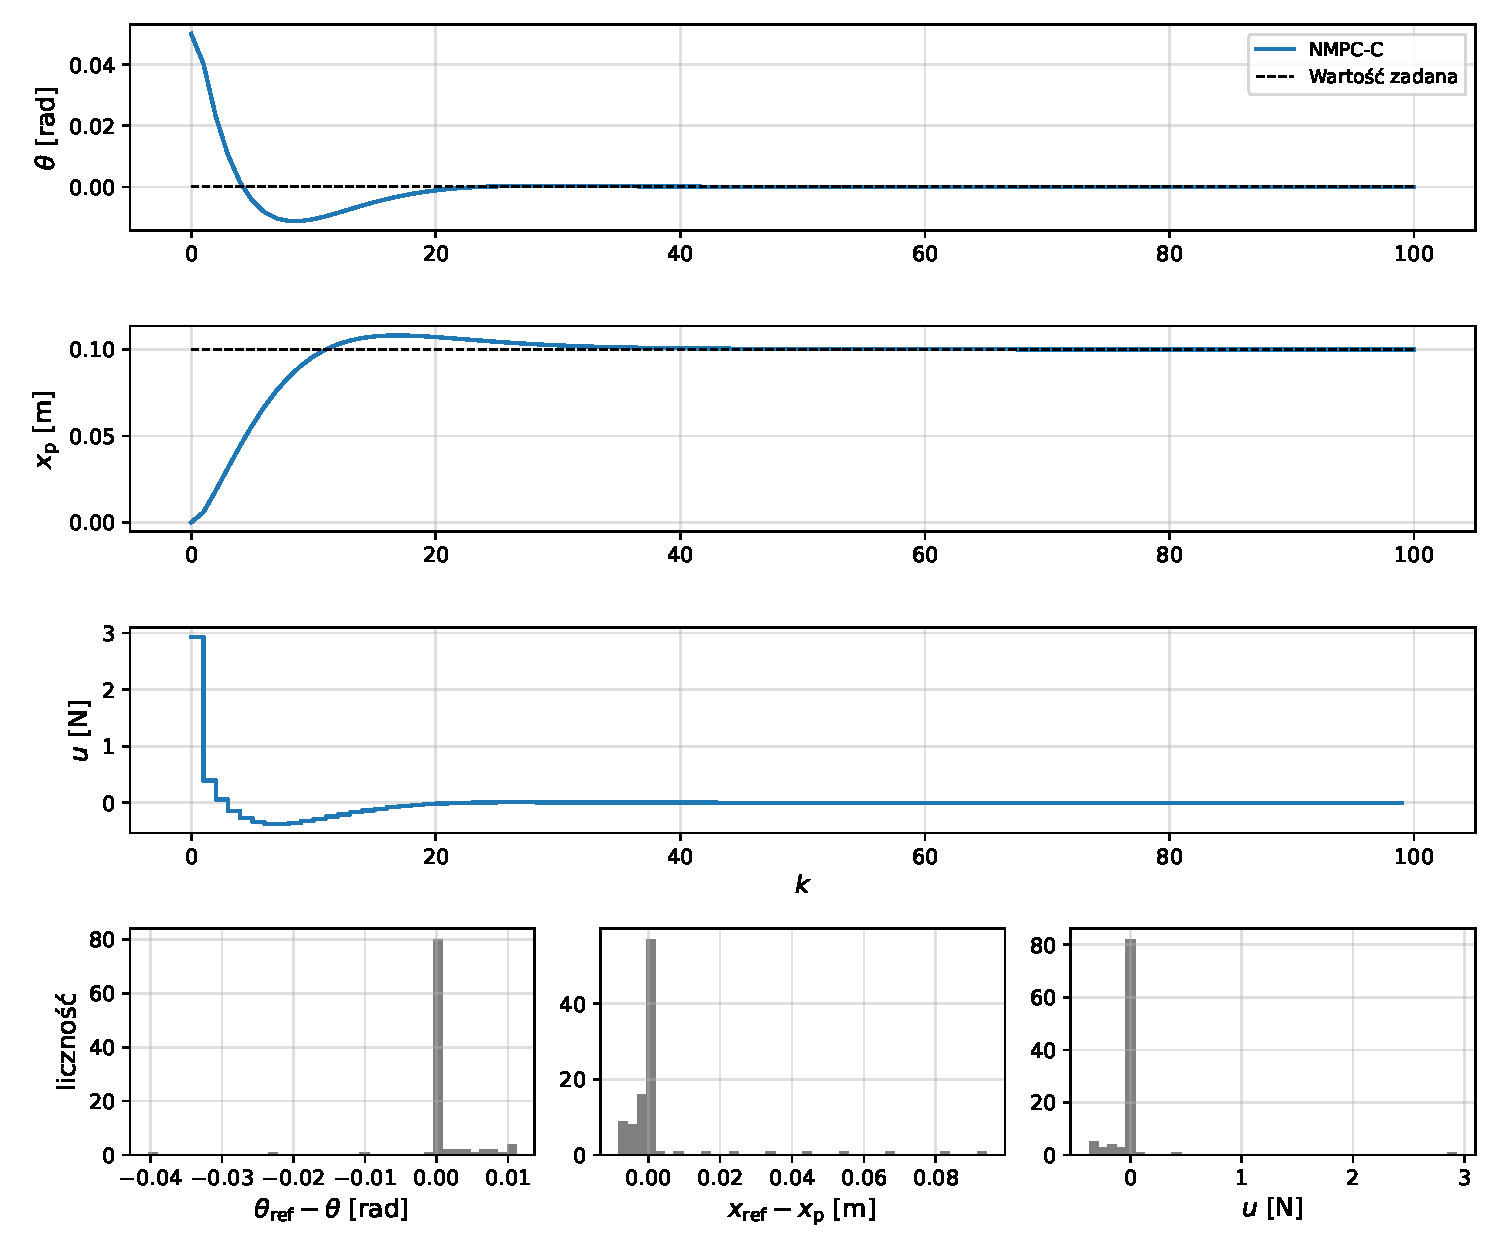
\includegraphics[width=\linewidth]{figs/S1_nmpc_c.pdf}
\caption{NMPC-C, Scenariusz S1 (nominalny): status automatyczny -- stabilny.}
\end{figure}
\clearpage
\begin{figure}[p]\centering
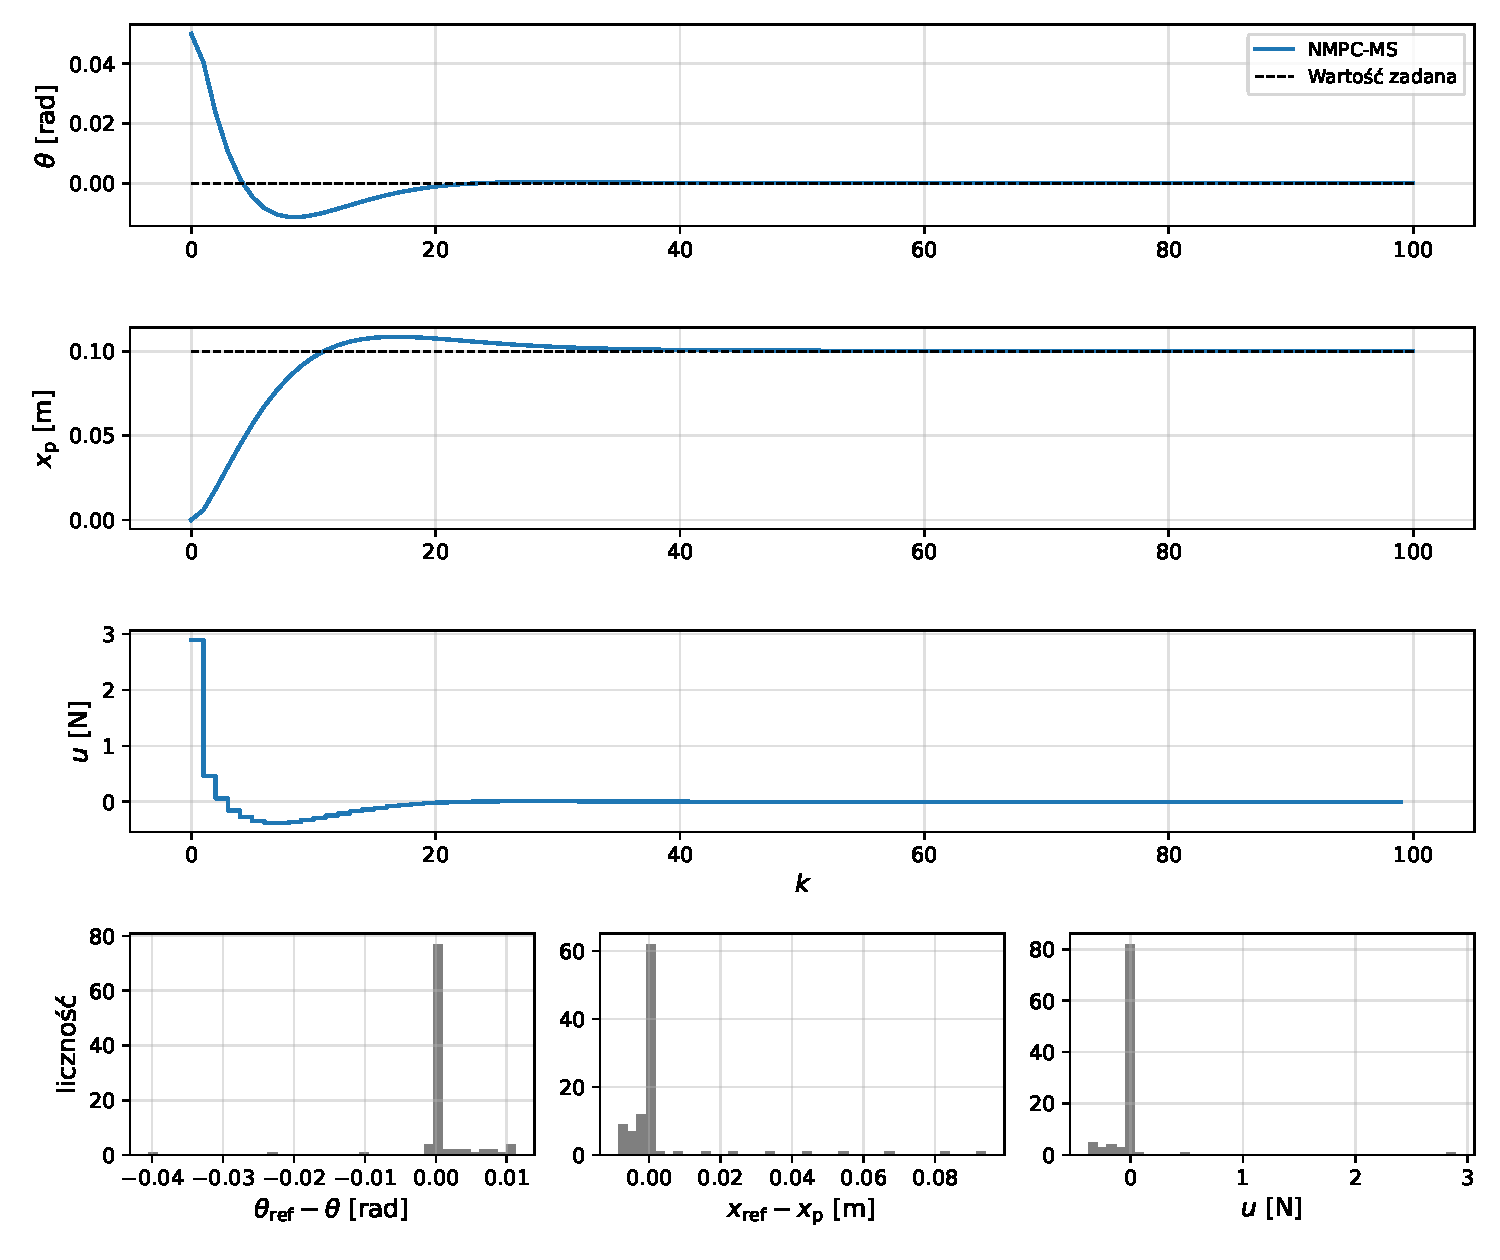
\includegraphics[width=\linewidth]{figs/S1_nmpc_ms.pdf}
\caption{NMPC-MS, Scenariusz S1 (nominalny): status automatyczny -- stabilny.}
\end{figure}
\clearpage
\begin{figure}[p]\centering
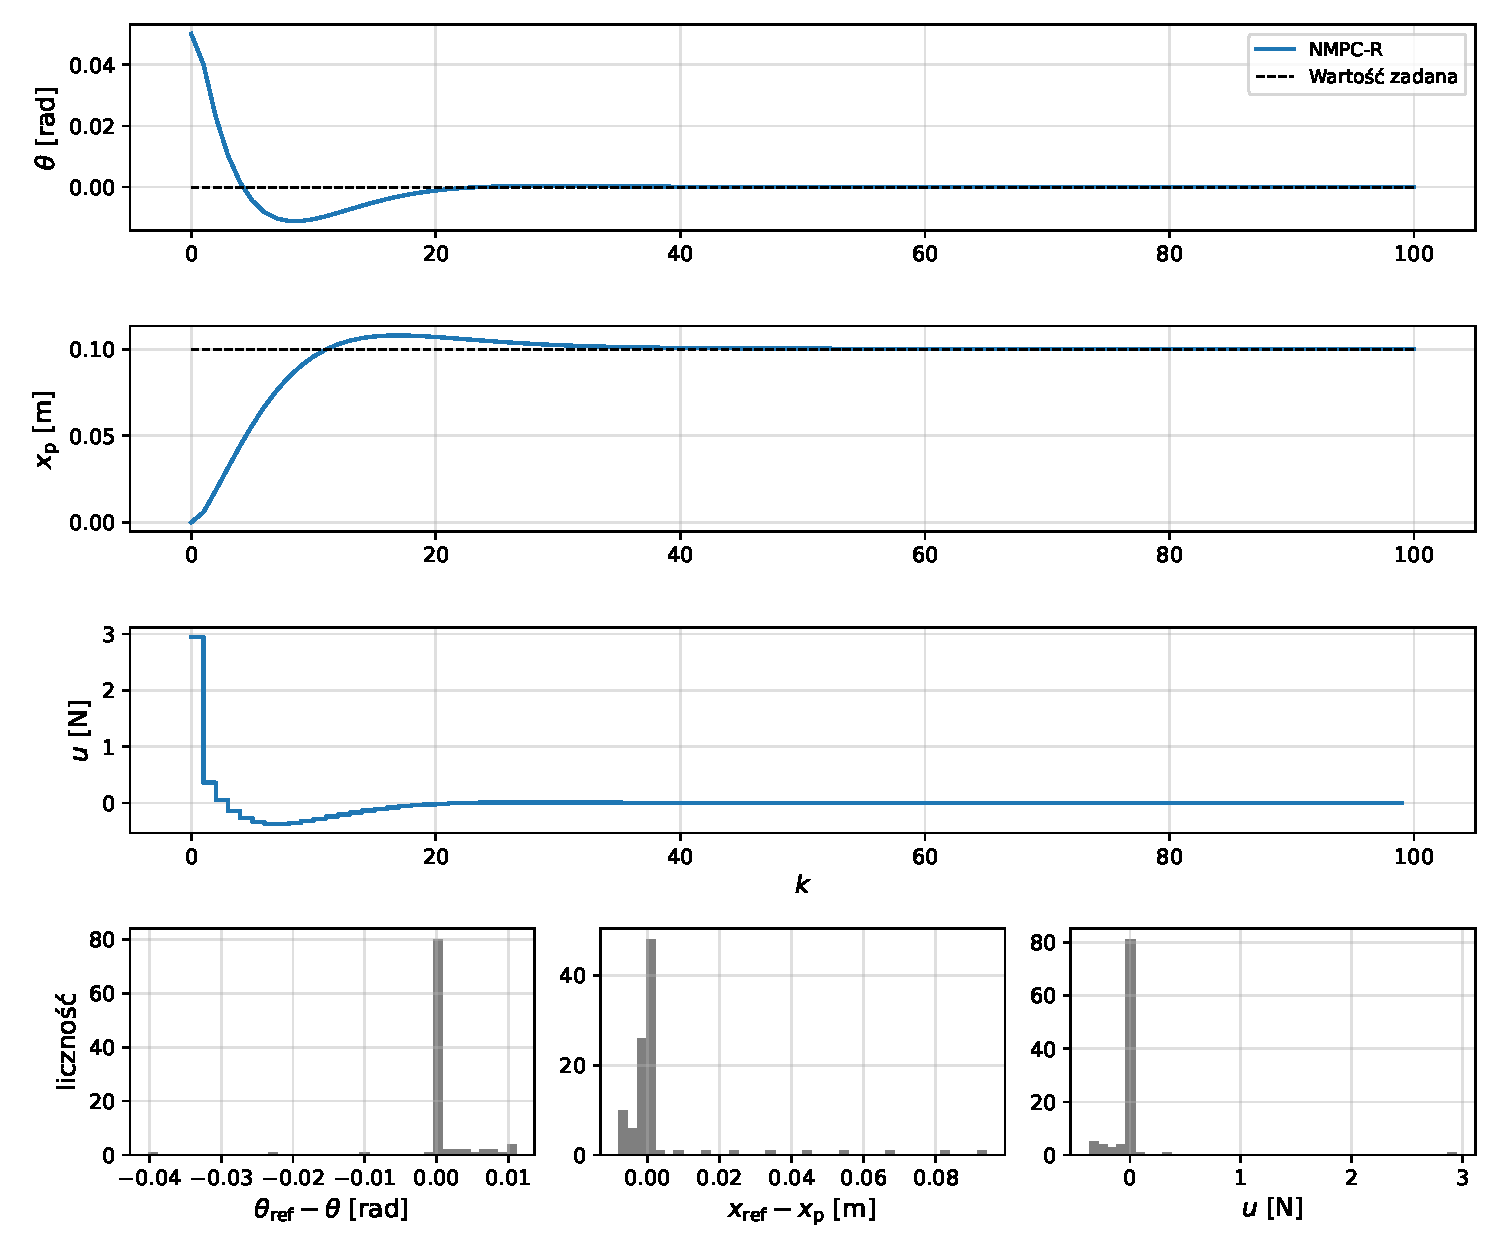
\includegraphics[width=\linewidth]{figs/S1_nmpc_r.pdf}
\caption{NMPC-R, Scenariusz S1 (nominalny): status automatyczny -- stabilny.}
\end{figure}
\clearpage
\begin{figure}[p]\centering
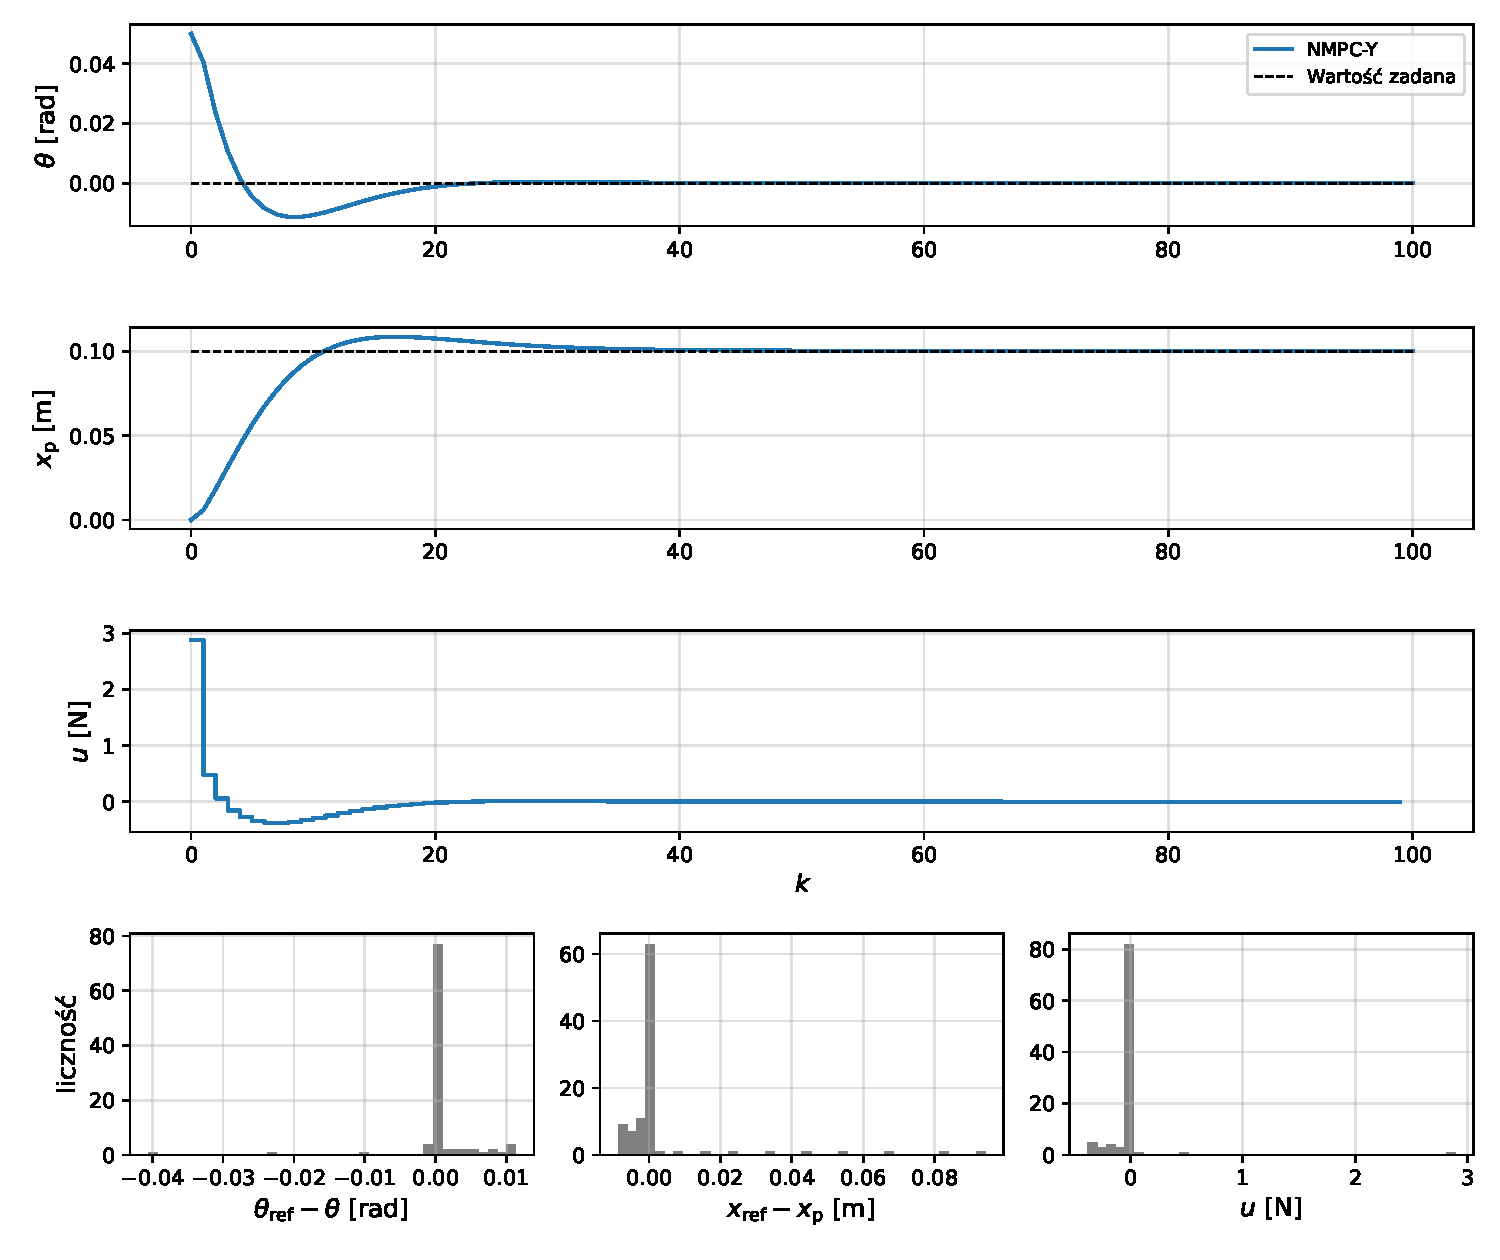
\includegraphics[width=\linewidth]{figs/S1_nmpc_y.pdf}
\caption{NMPC-Y, Scenariusz S1 (nominalny): status automatyczny -- stabilny.}
\end{figure}
\clearpage
\subsection{Przebiegi -- Scenariusz S2 (skoki zakłócenia)}
\begin{figure}[p]\centering
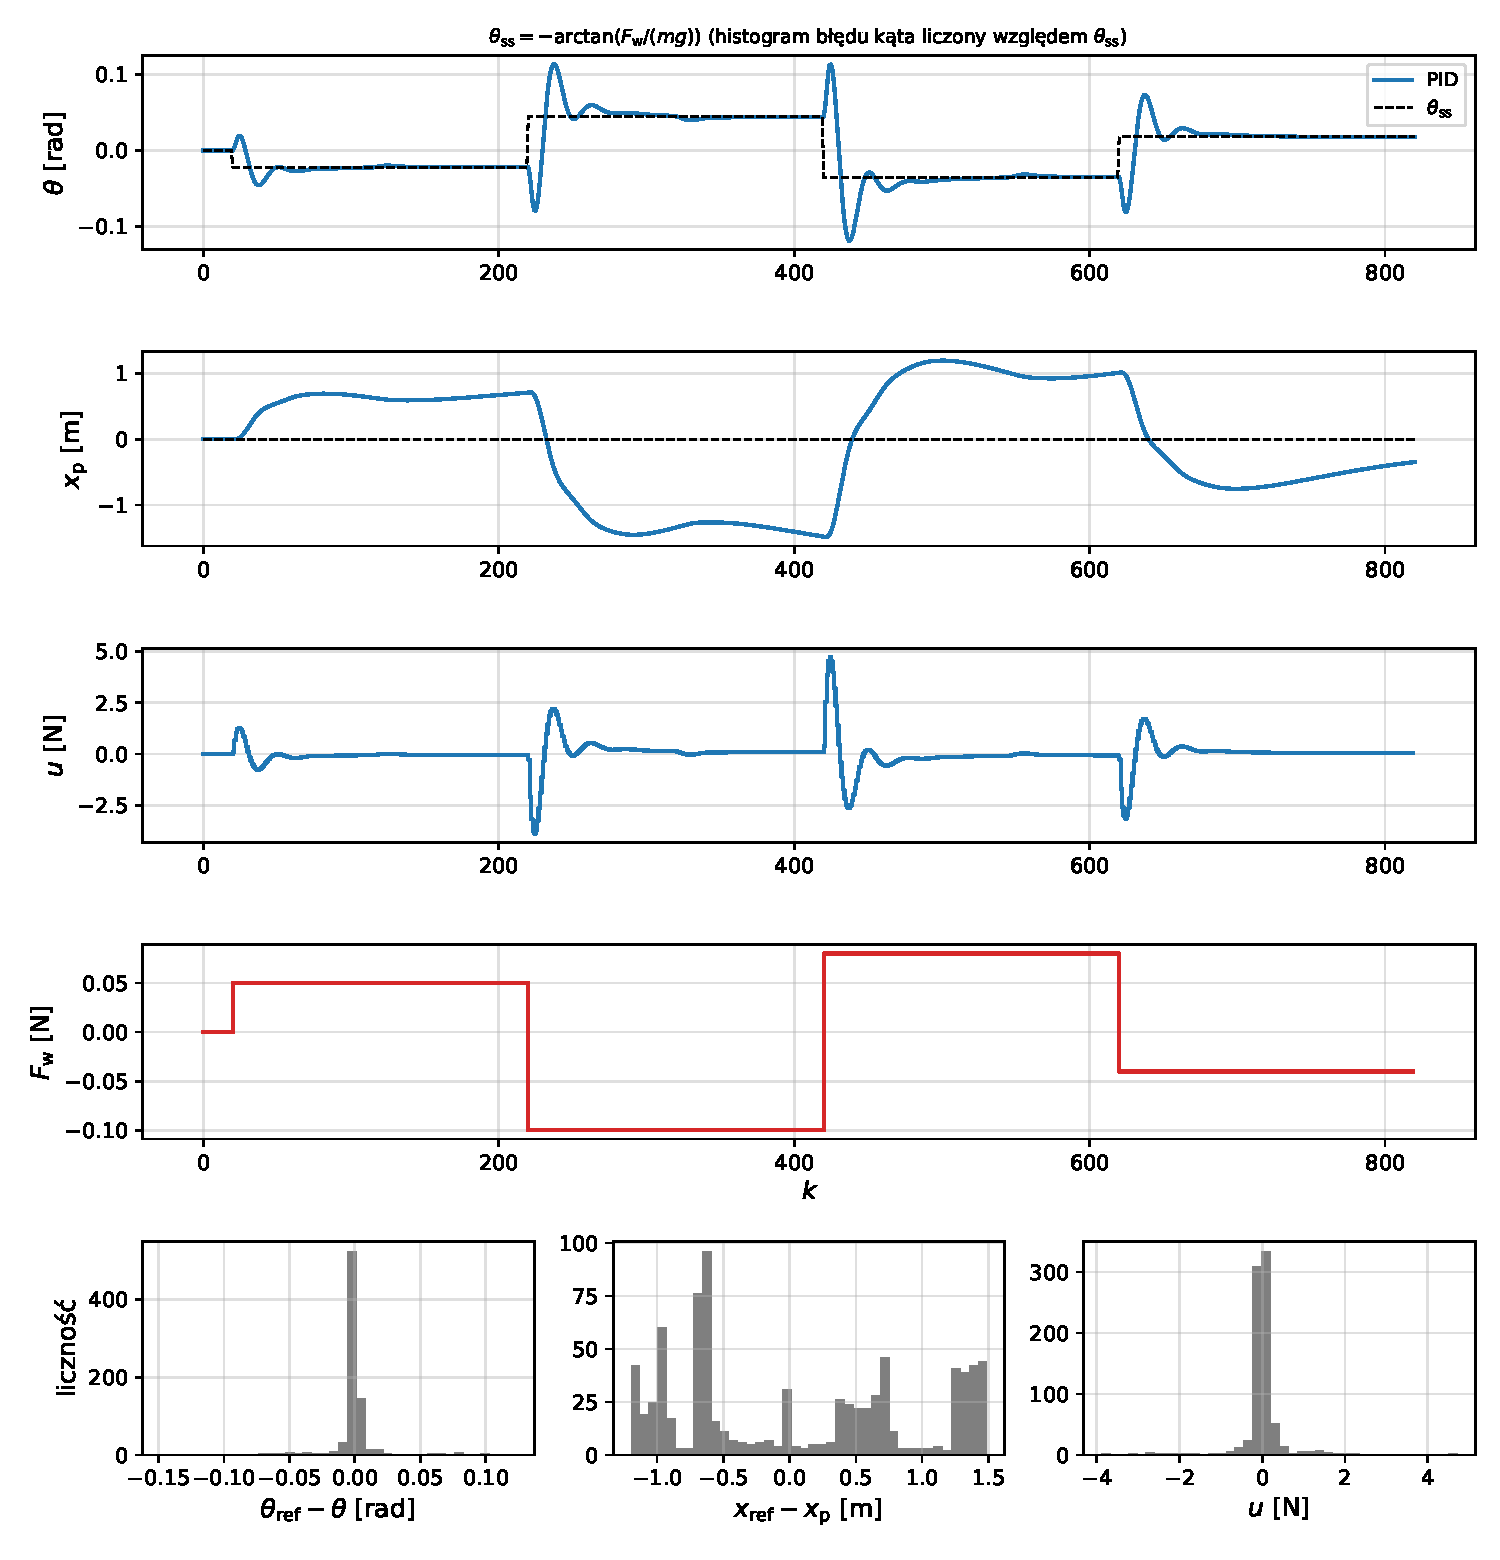
\includegraphics[width=\linewidth]{figs/S2_pid.pdf}
\caption{PID, Scenariusz S2 (skoki zakłócenia): status automatyczny -- \textbf{nieustalony}.}
\end{figure}
\clearpage
\begin{figure}[p]\centering
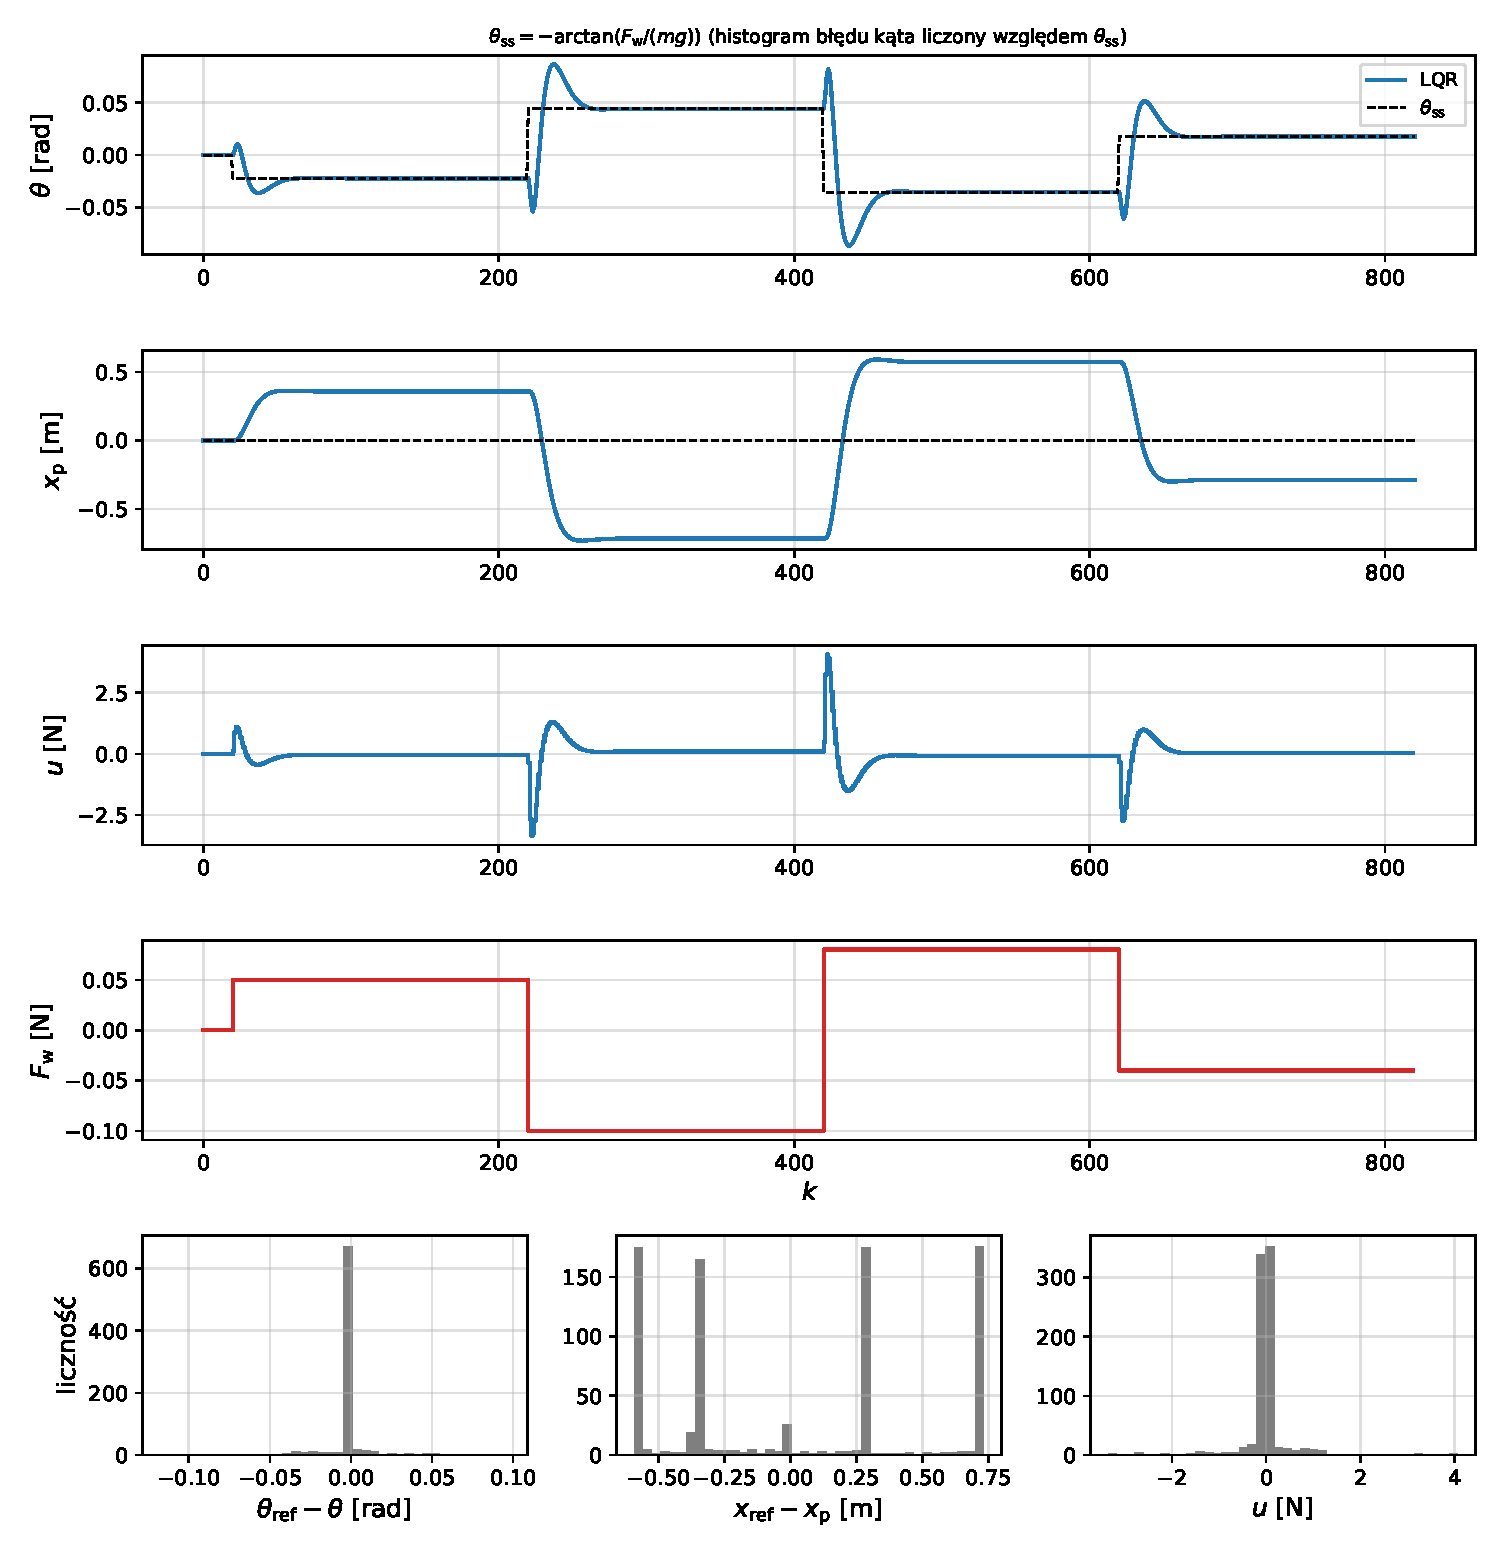
\includegraphics[width=\linewidth]{figs/S2_lqr.pdf}
\caption{LQR, Scenariusz S2 (skoki zakłócenia): status automatyczny -- stabilny.}
\end{figure}
\clearpage
\begin{figure}[p]\centering
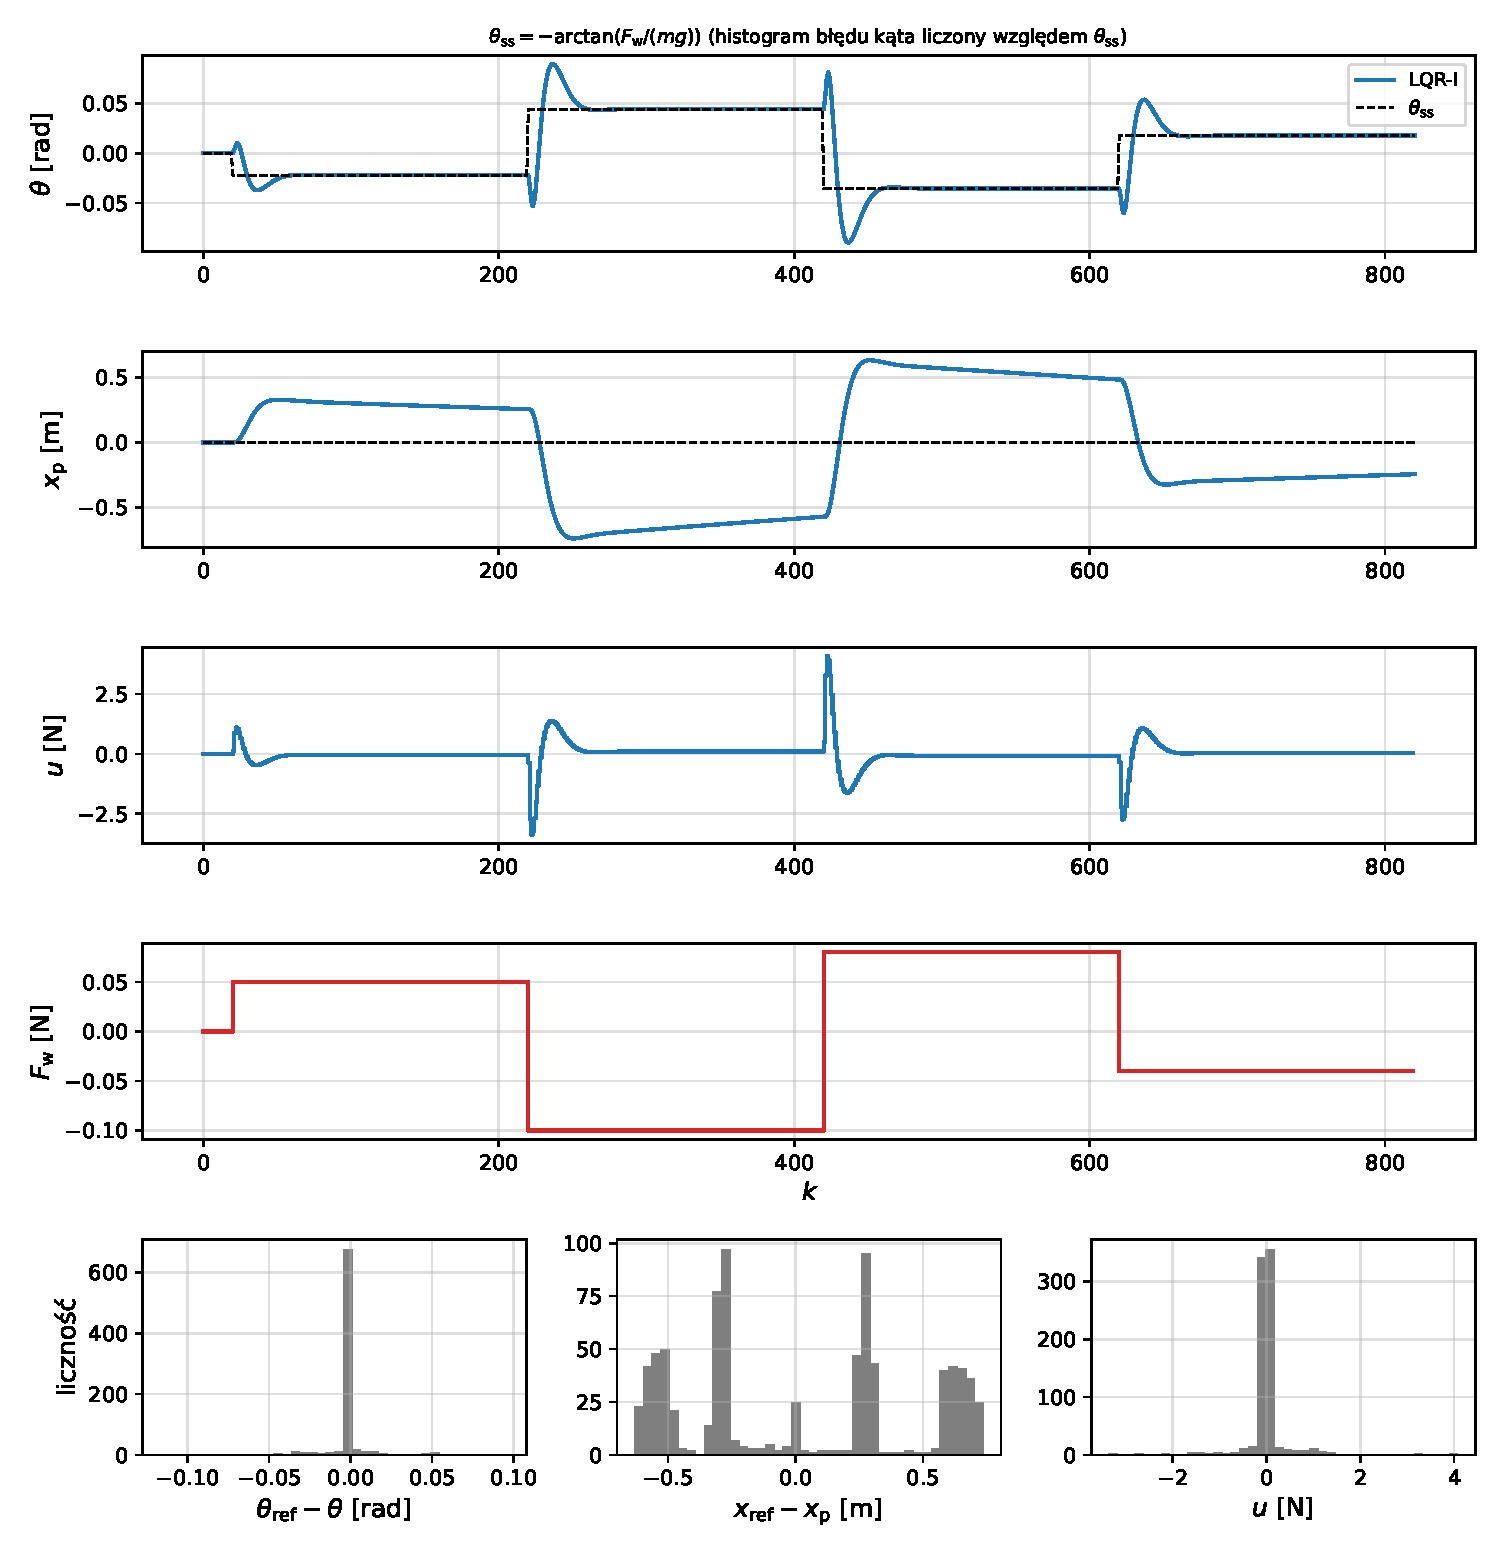
\includegraphics[width=\linewidth]{figs/S2_lqr_i.pdf}
\caption{LQR-I, Scenariusz S2 (skoki zakłócenia): status automatyczny -- stabilny.}
\end{figure}
\clearpage
\begin{figure}[p]\centering
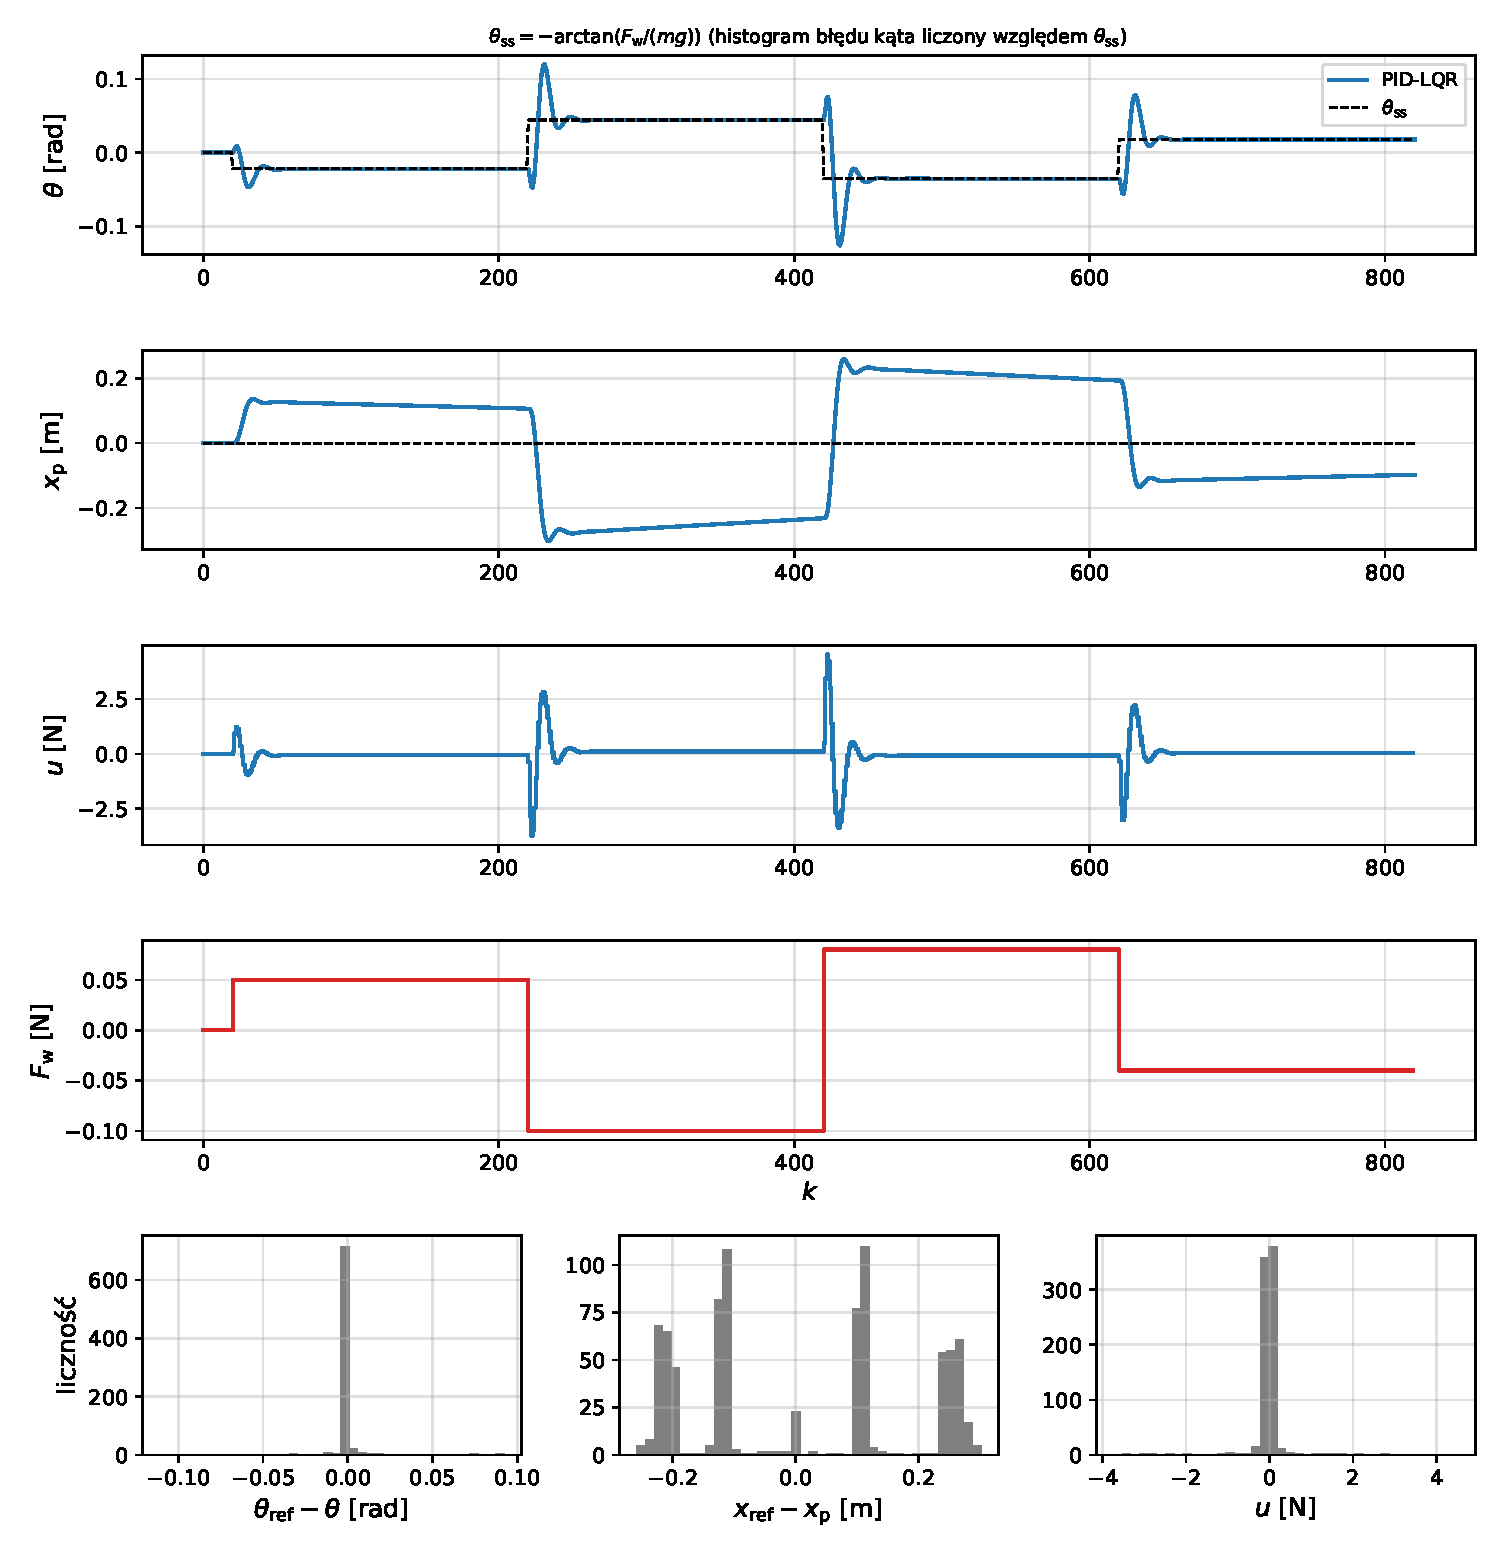
\includegraphics[width=\linewidth]{figs/S2_pid_lqr.pdf}
\caption{PID-LQR, Scenariusz S2 (skoki zakłócenia): status automatyczny -- stabilny.}
\end{figure}
\clearpage
\begin{figure}[p]\centering
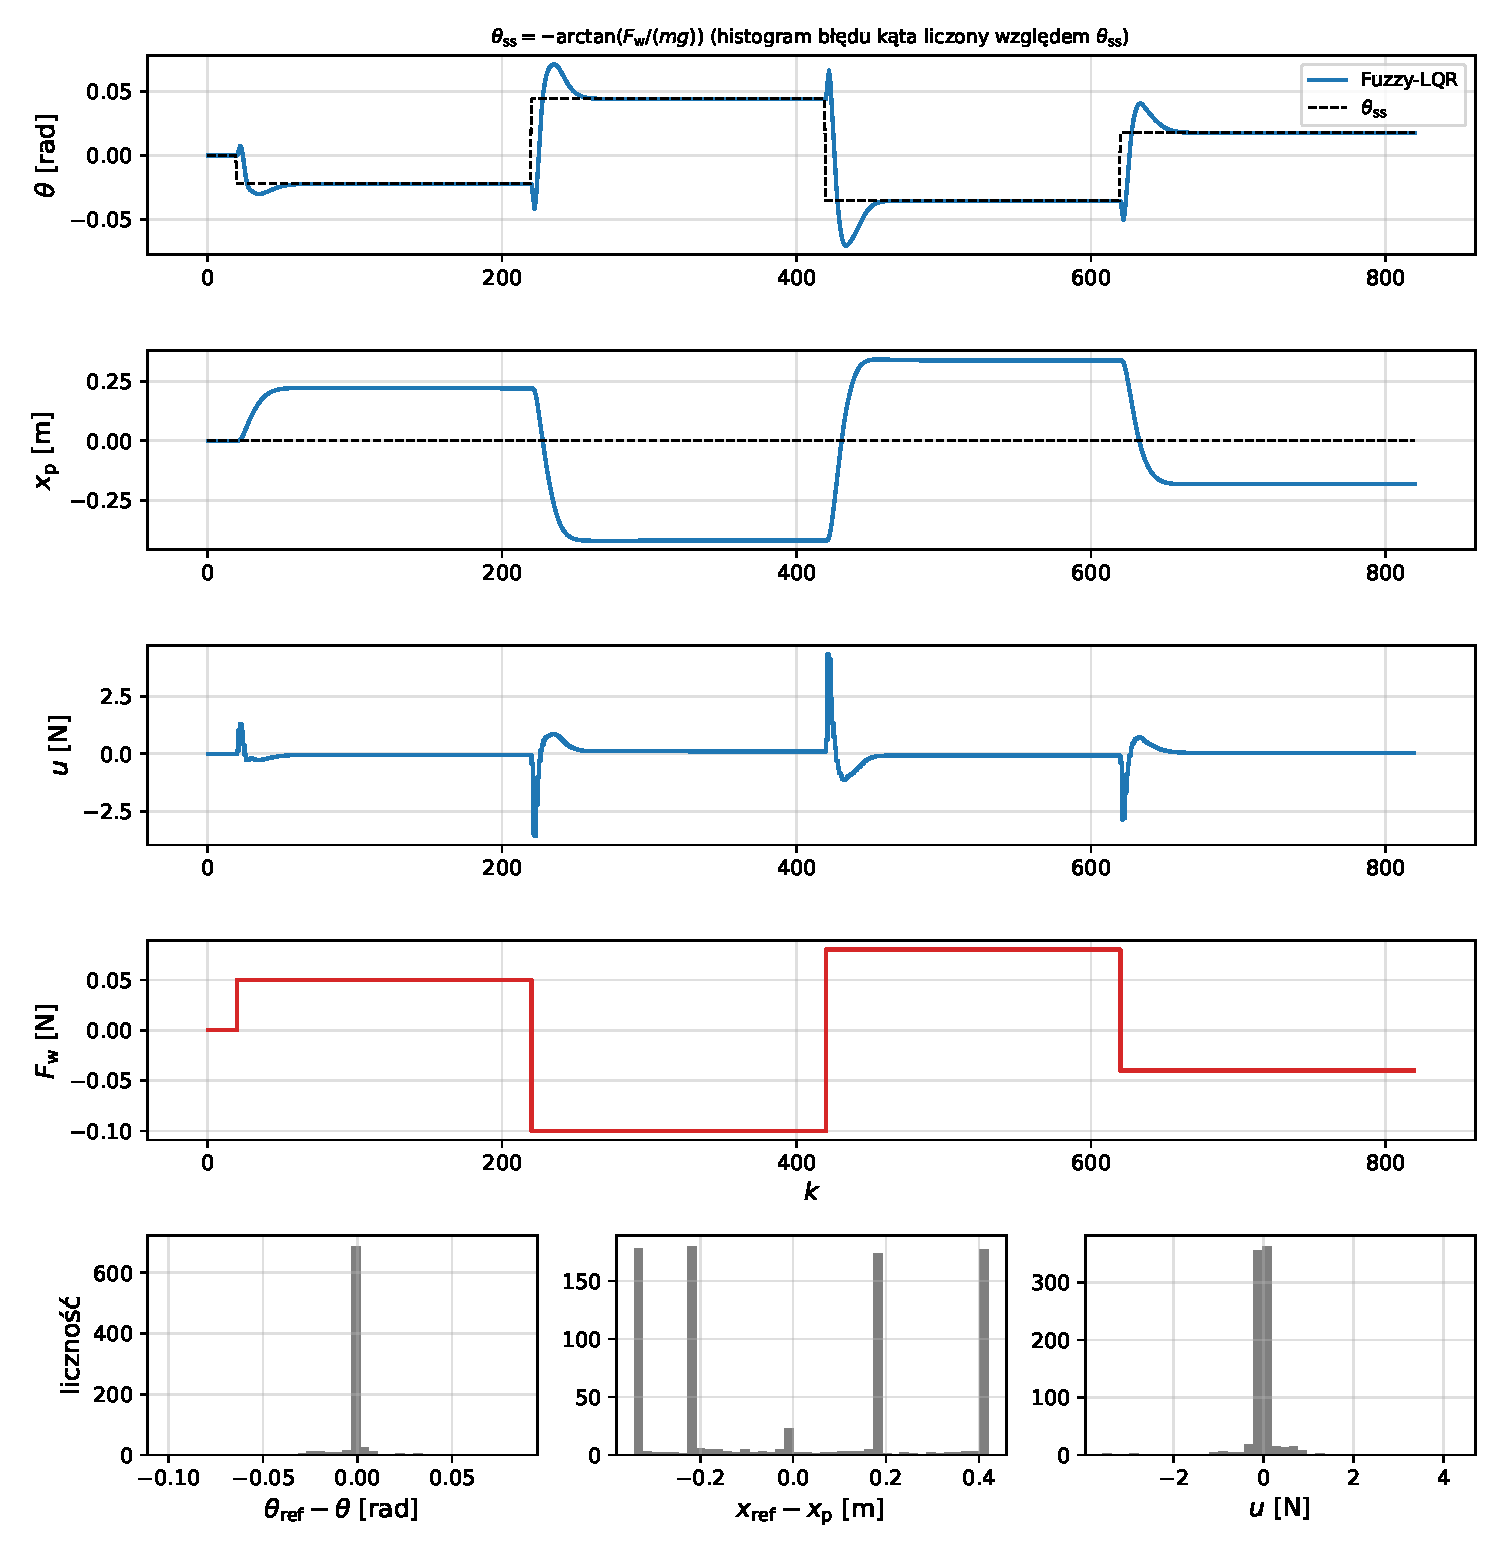
\includegraphics[width=\linewidth]{figs/S2_fuzzy_lqr.pdf}
\caption{Fuzzy-LQR, Scenariusz S2 (skoki zakłócenia): status automatyczny -- stabilny.}
\end{figure}
\clearpage
\begin{figure}[p]\centering
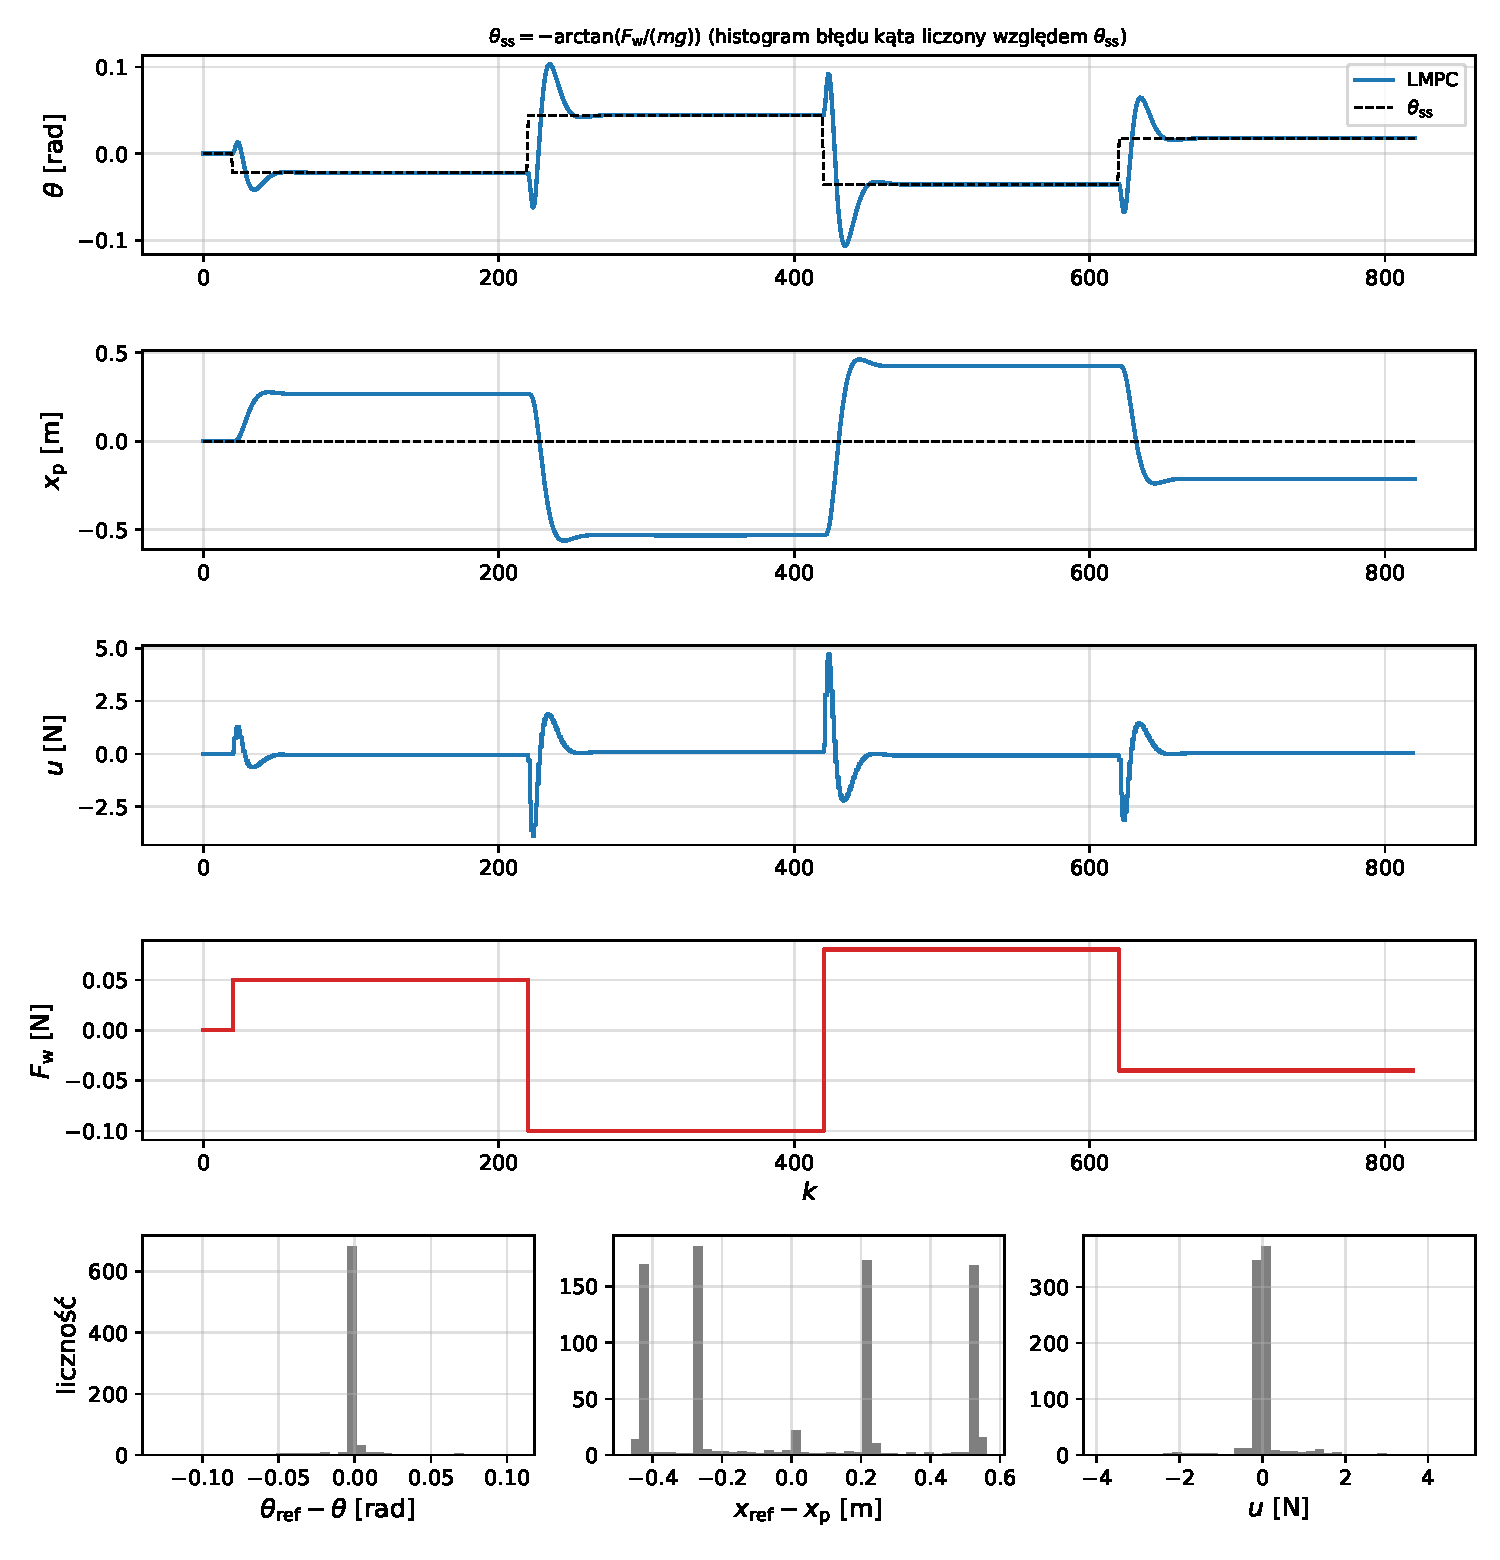
\includegraphics[width=\linewidth]{figs/S2_lmpc.pdf}
\caption{LMPC, Scenariusz S2 (skoki zakłócenia): status automatyczny -- stabilny.}
\end{figure}
\clearpage
\begin{figure}[p]\centering
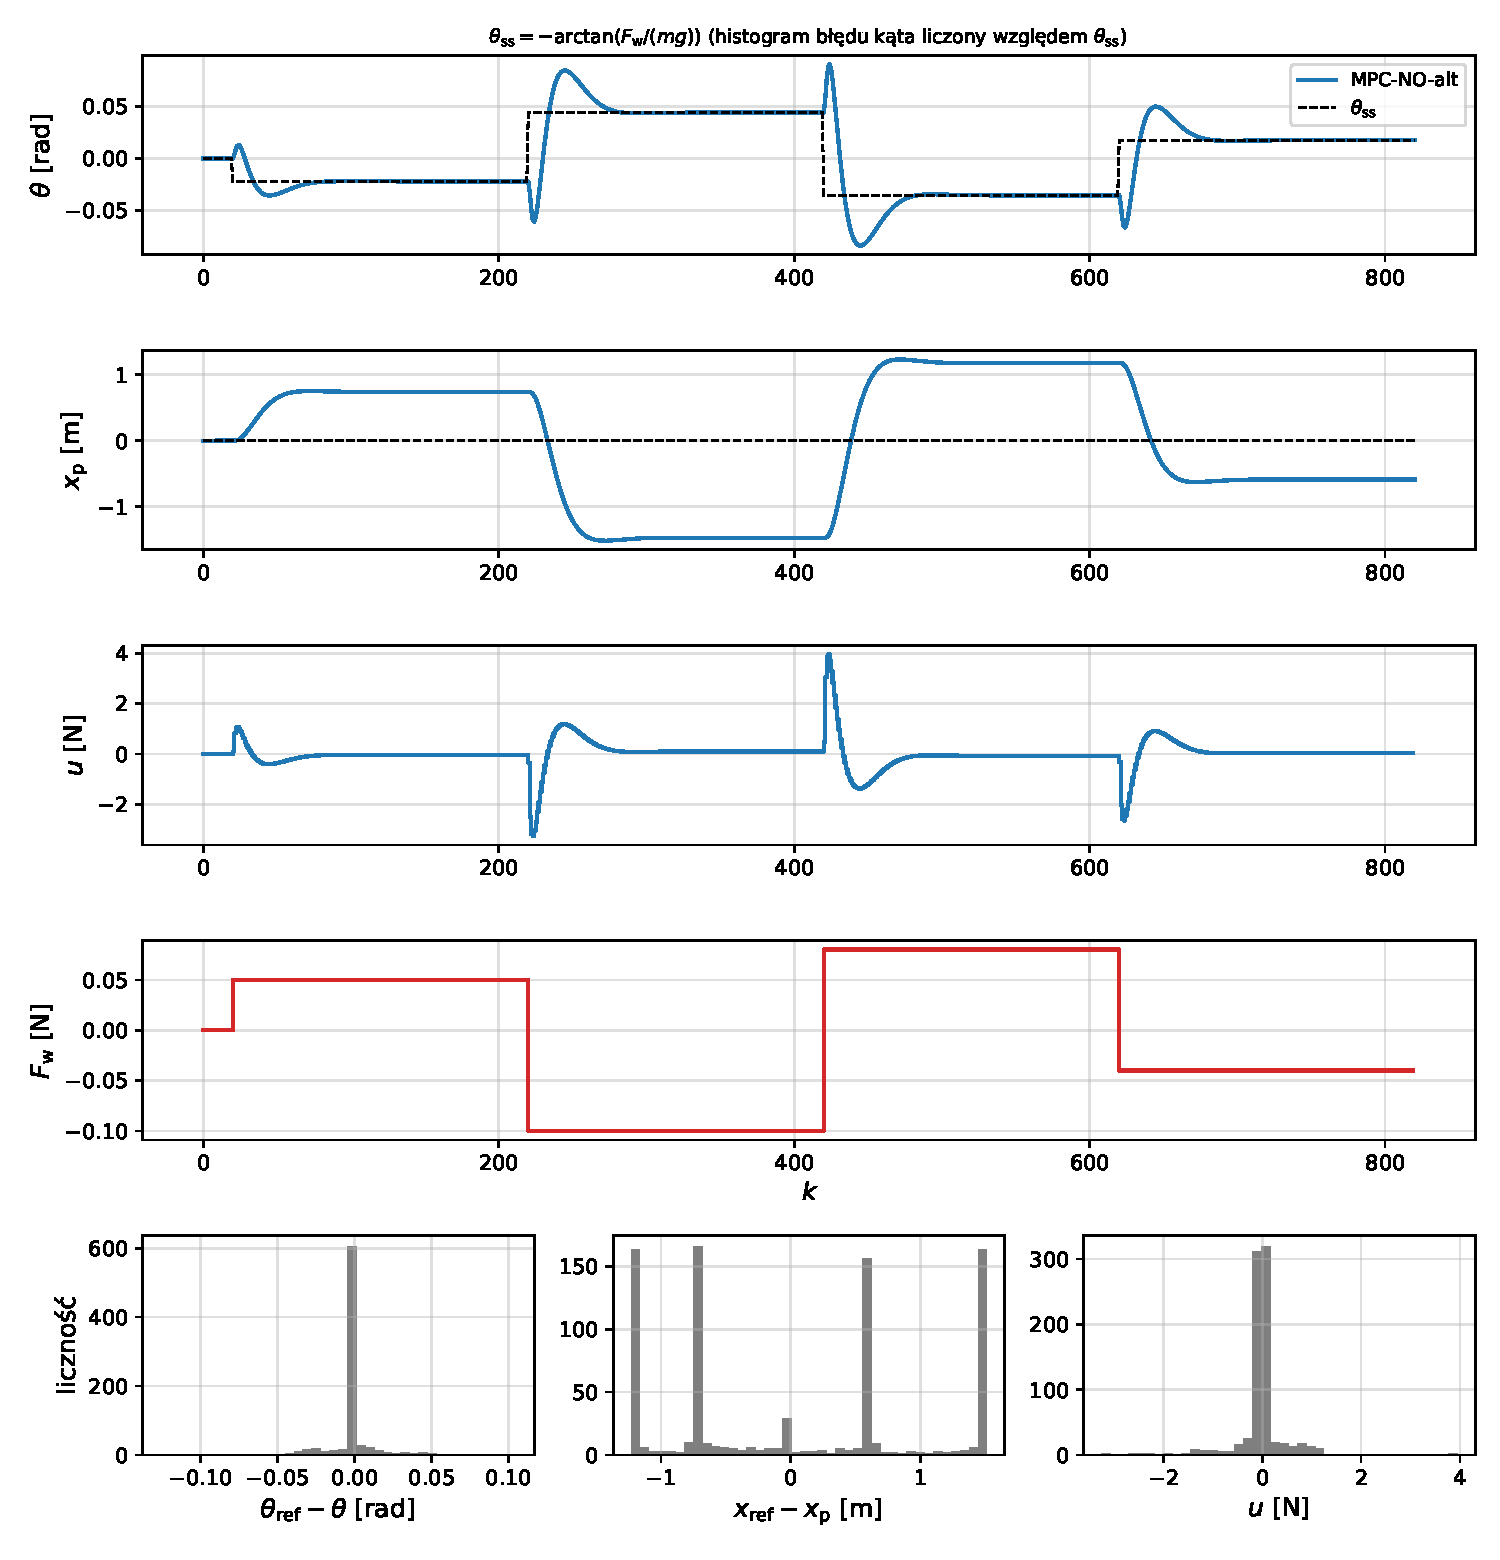
\includegraphics[width=\linewidth]{figs/S2_mpc_no_alt.pdf}
\caption{MPC-NO-alt, Scenariusz S2 (skoki zakłócenia): status automatyczny -- stabilny.}
\end{figure}
\clearpage
\begin{figure}[p]\centering
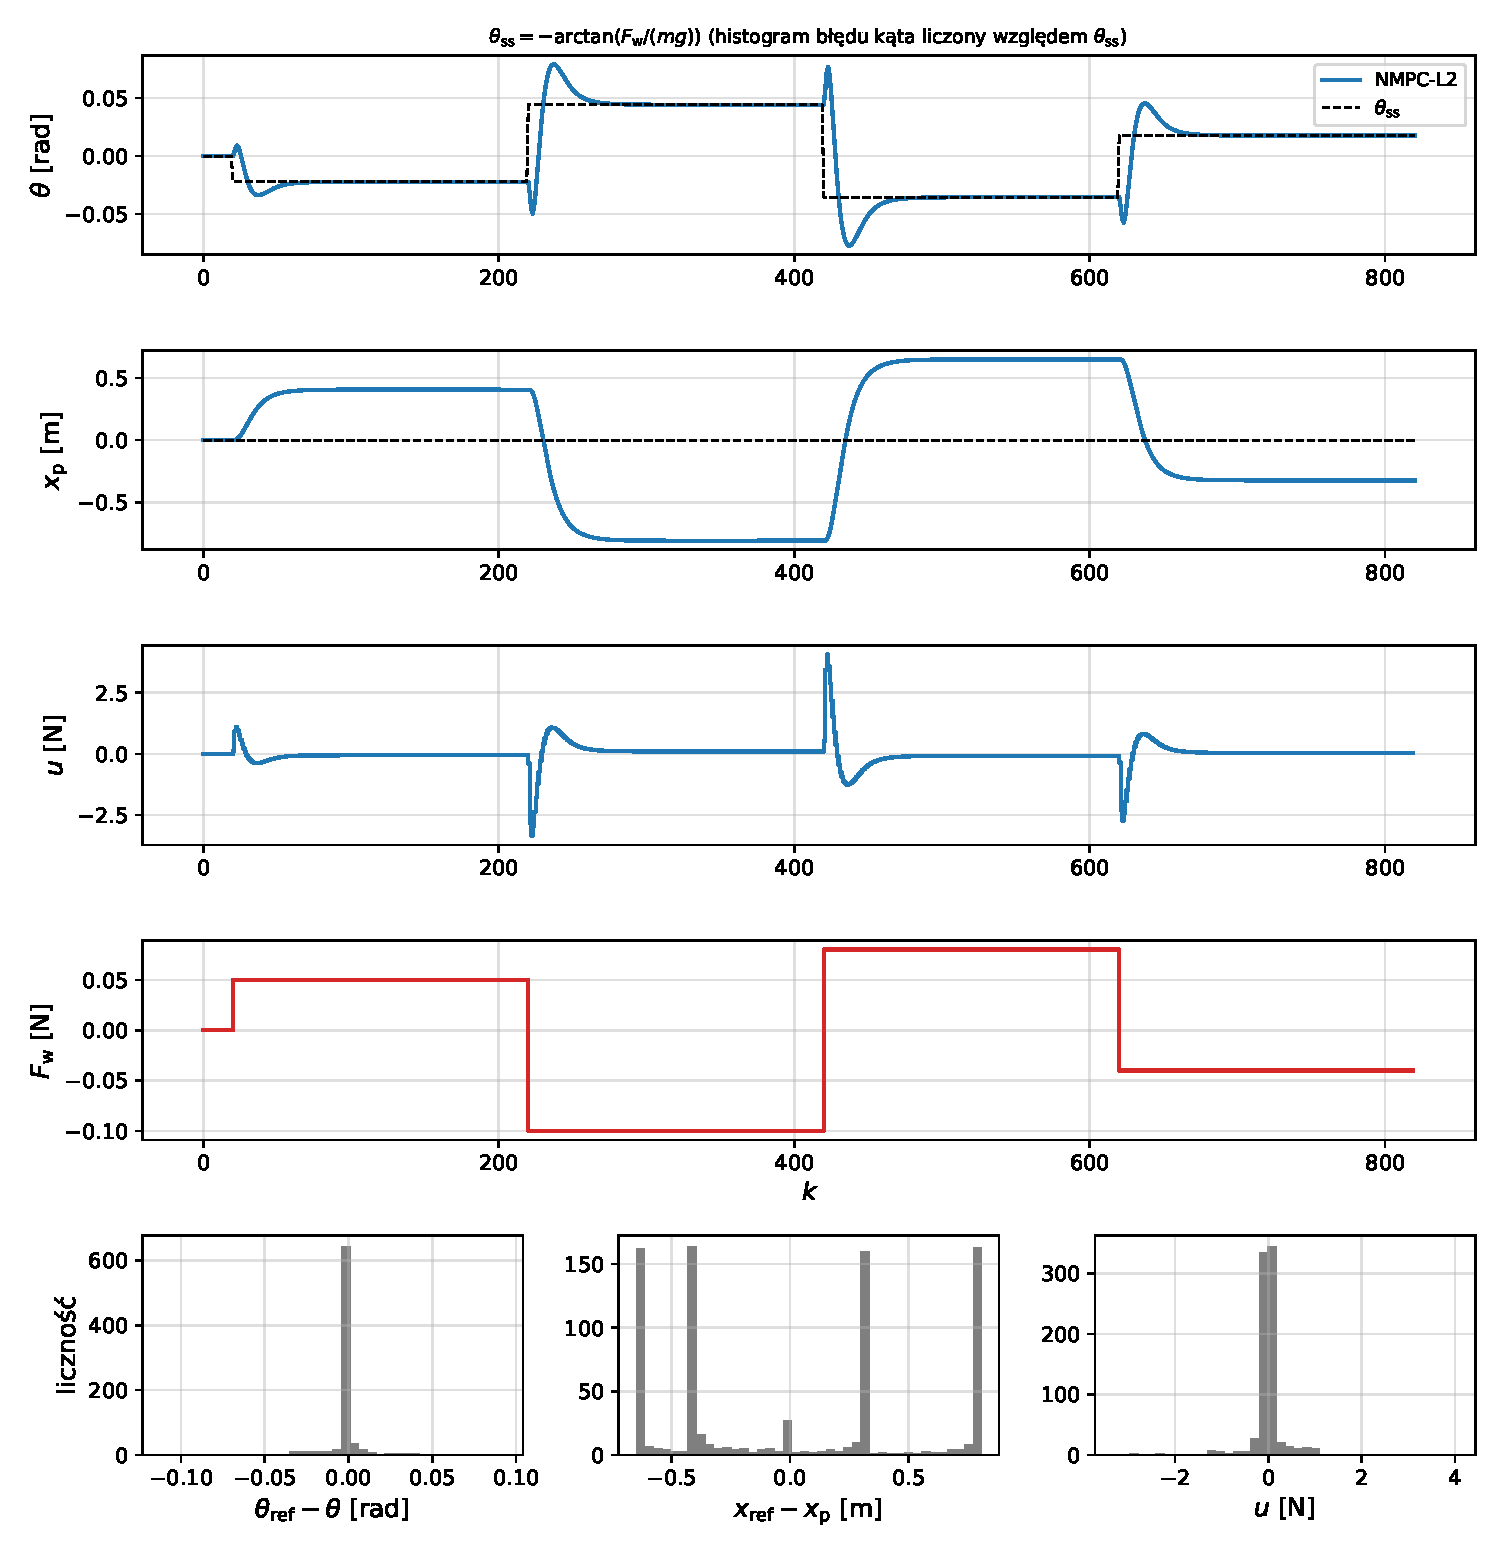
\includegraphics[width=\linewidth]{figs/S2_nmpc_l2.pdf}
\caption{NMPC-L$_2$, Scenariusz S2 (skoki zakłócenia): status automatyczny -- stabilny.}
\end{figure}
\clearpage
\begin{figure}[p]\centering
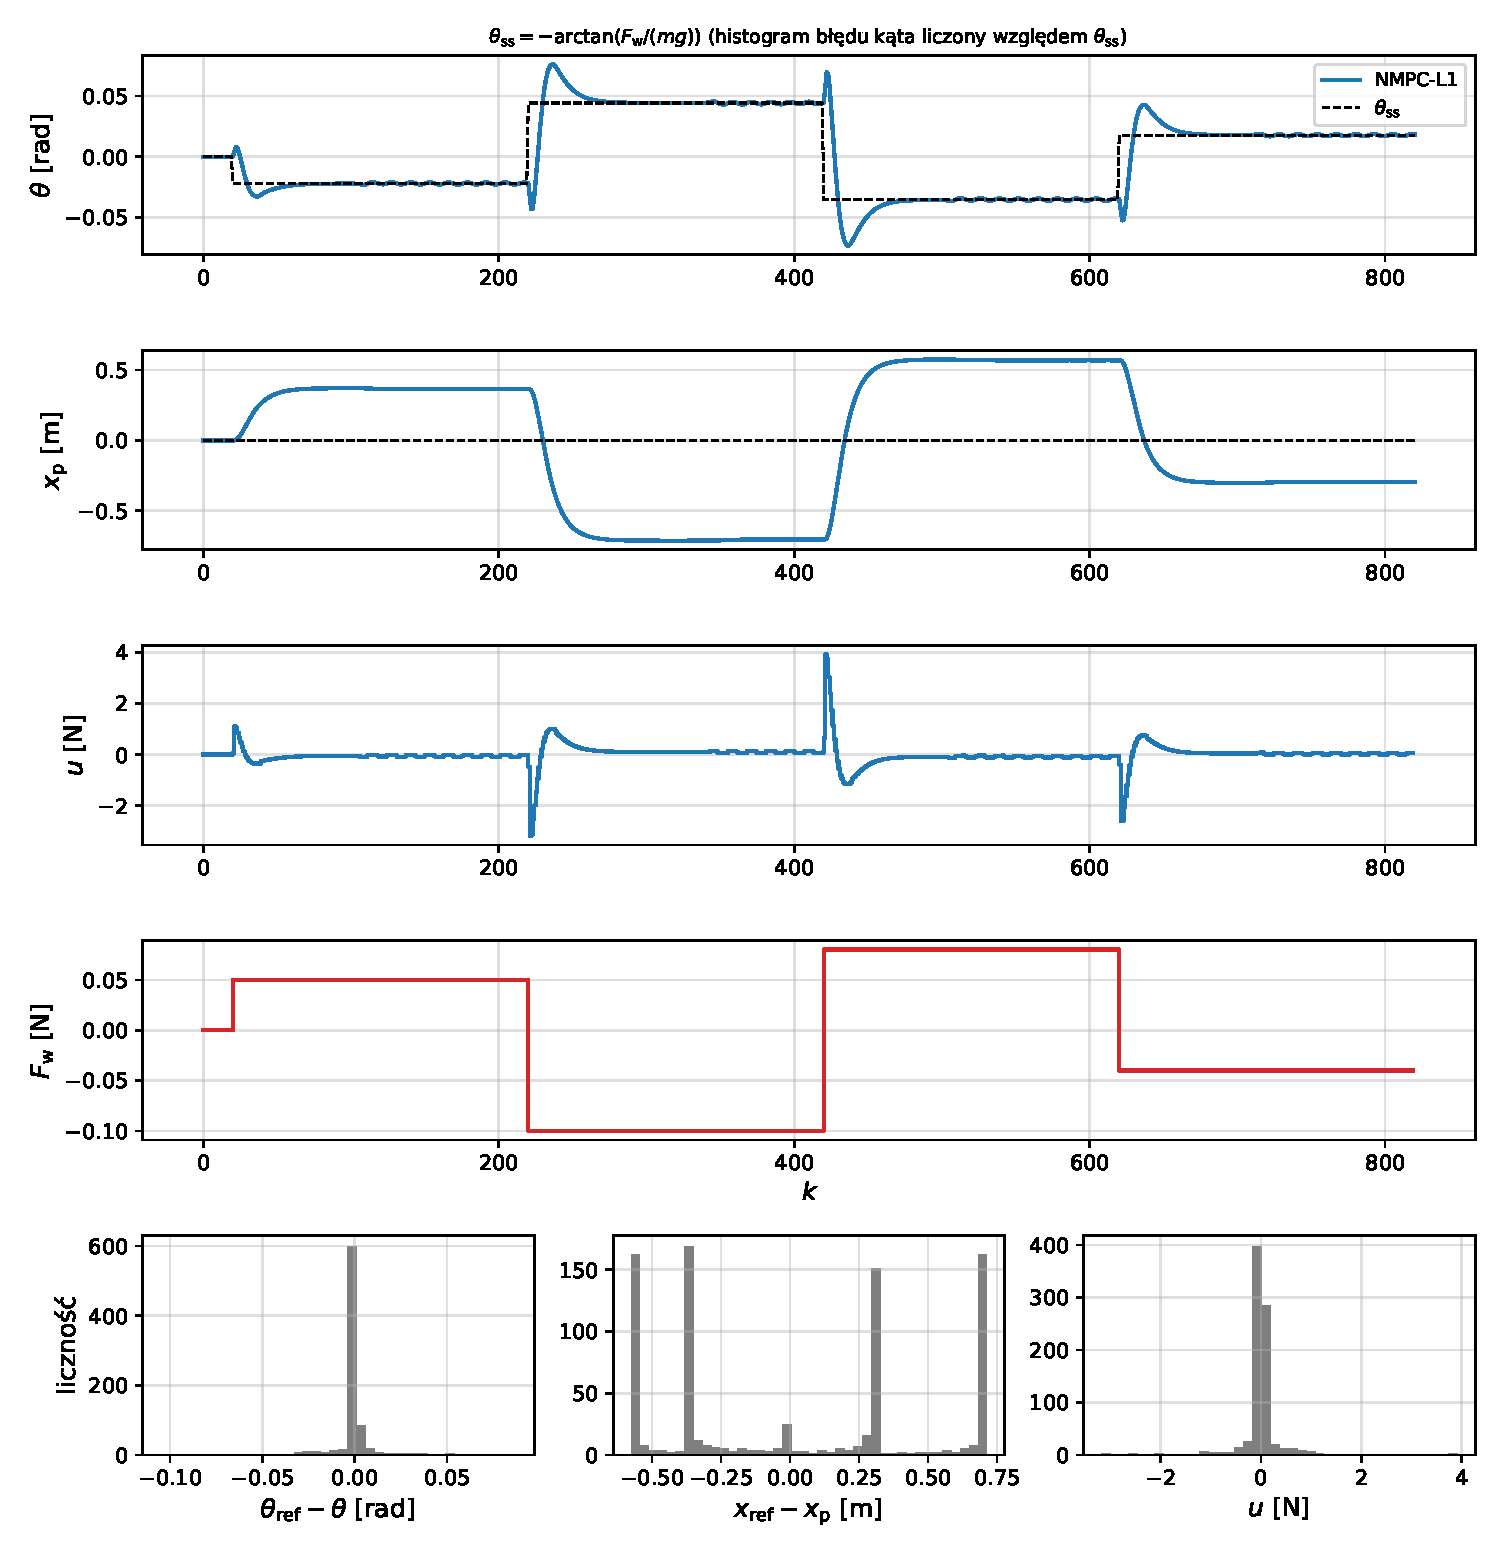
\includegraphics[width=\linewidth]{figs/S2_nmpc_l1.pdf}
\caption{NMPC-L$_1$, Scenariusz S2 (skoki zakłócenia): status automatyczny -- stabilny.}
\end{figure}
\clearpage
\begin{figure}[p]\centering
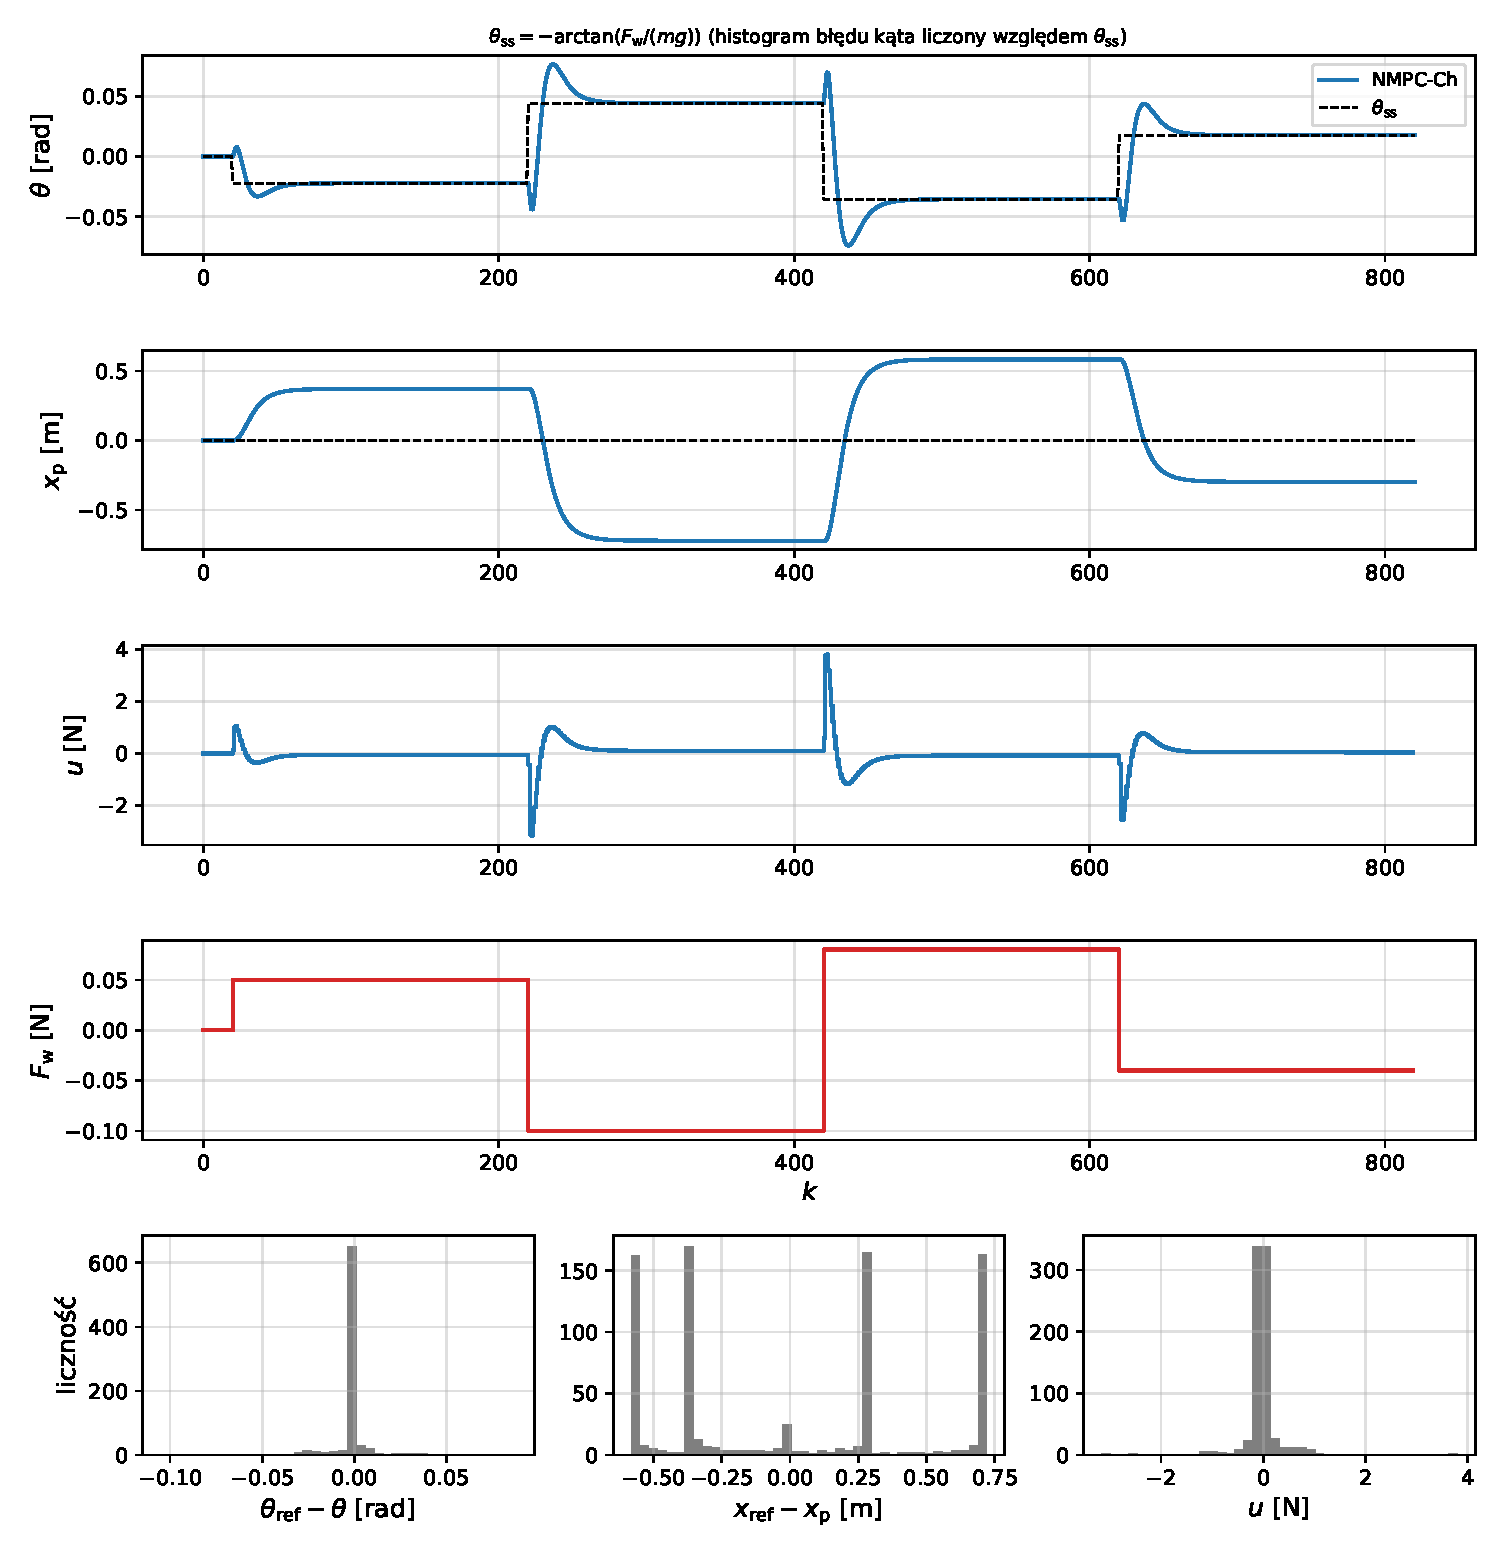
\includegraphics[width=\linewidth]{figs/S2_nmpc_ch.pdf}
\caption{NMPC-Ch, Scenariusz S2 (skoki zakłócenia): status automatyczny -- stabilny.}
\end{figure}
\clearpage
\begin{figure}[p]\centering
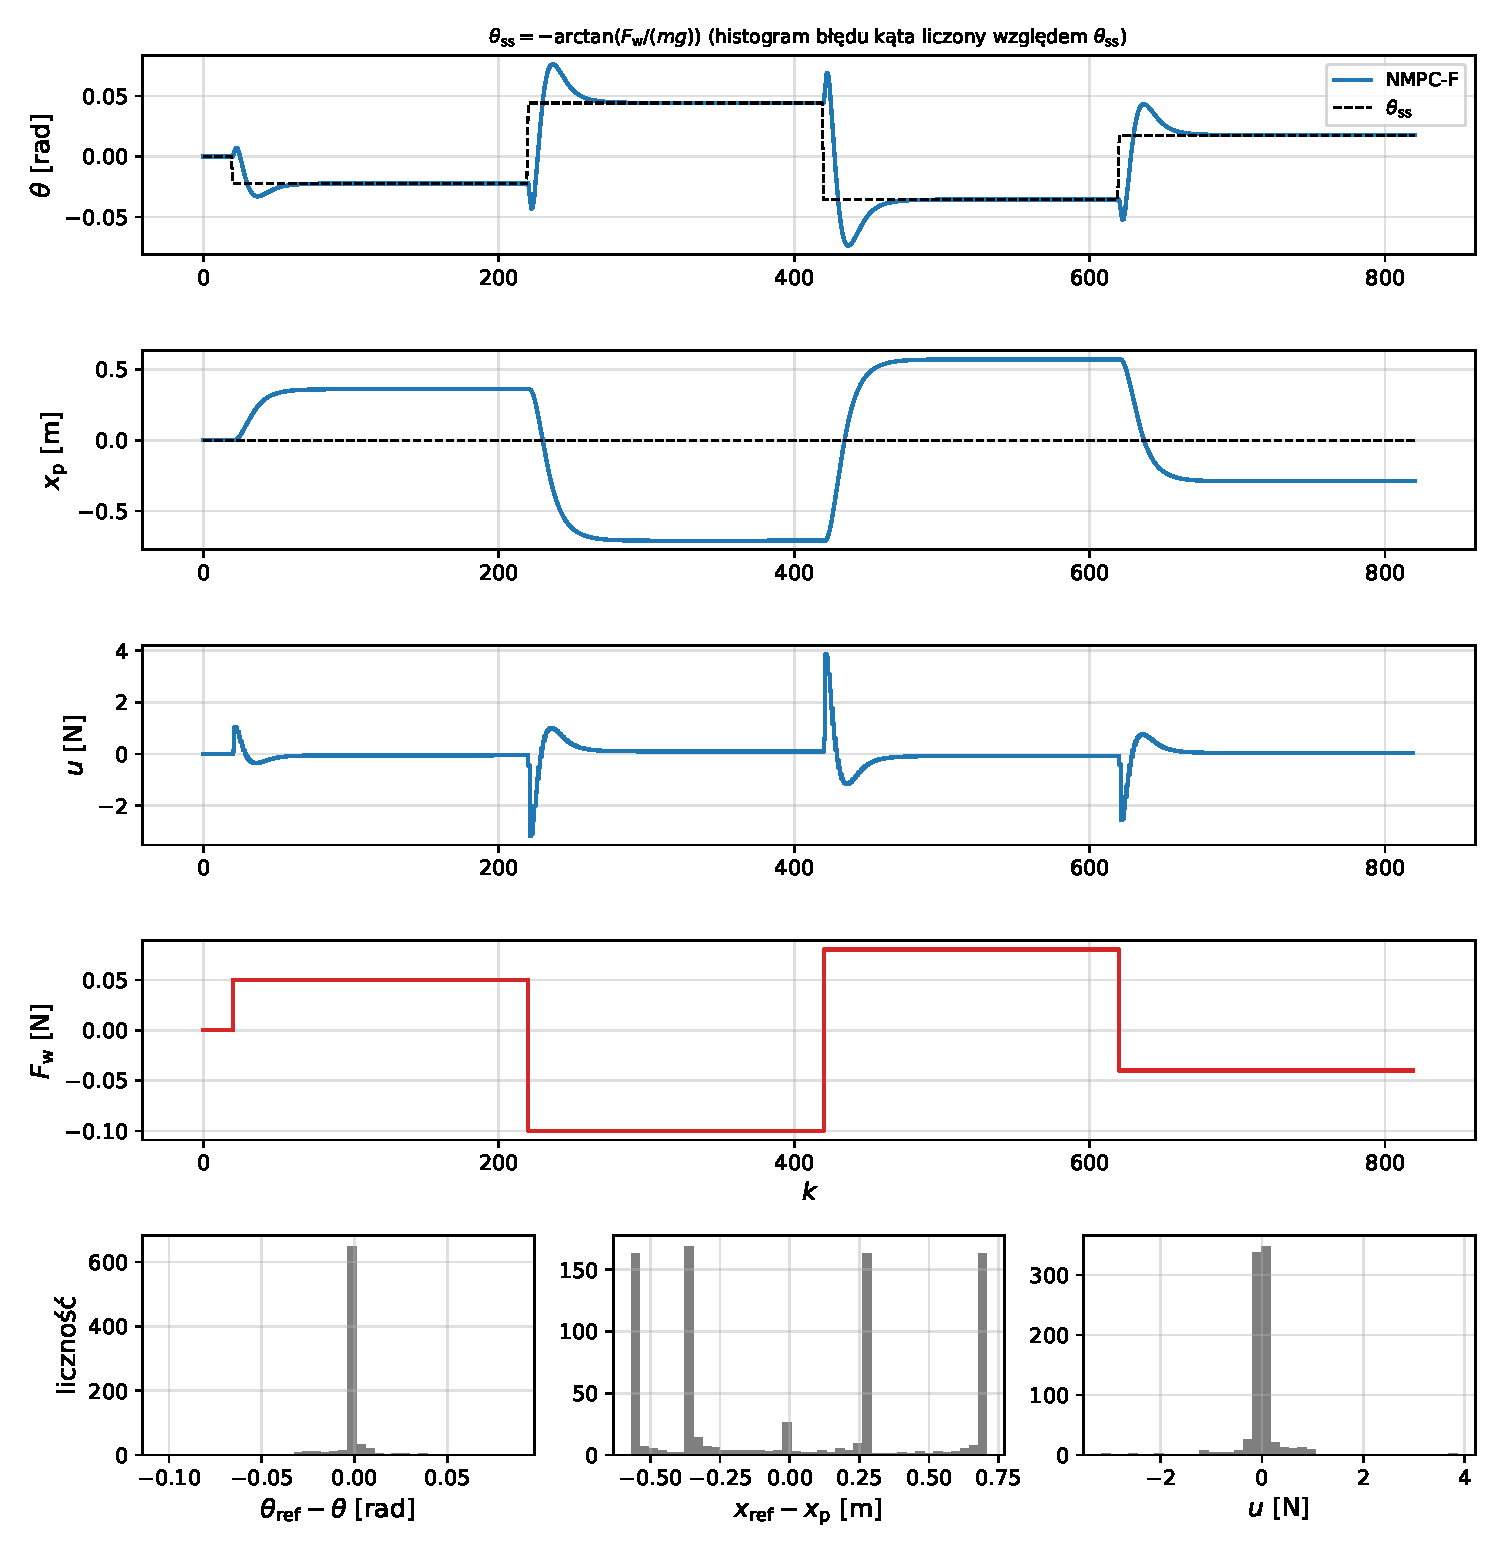
\includegraphics[width=\linewidth]{figs/S2_nmpc_f.pdf}
\caption{NMPC-F, Scenariusz S2 (skoki zakłócenia): status automatyczny -- stabilny.}
\end{figure}
\clearpage
\begin{figure}[p]\centering
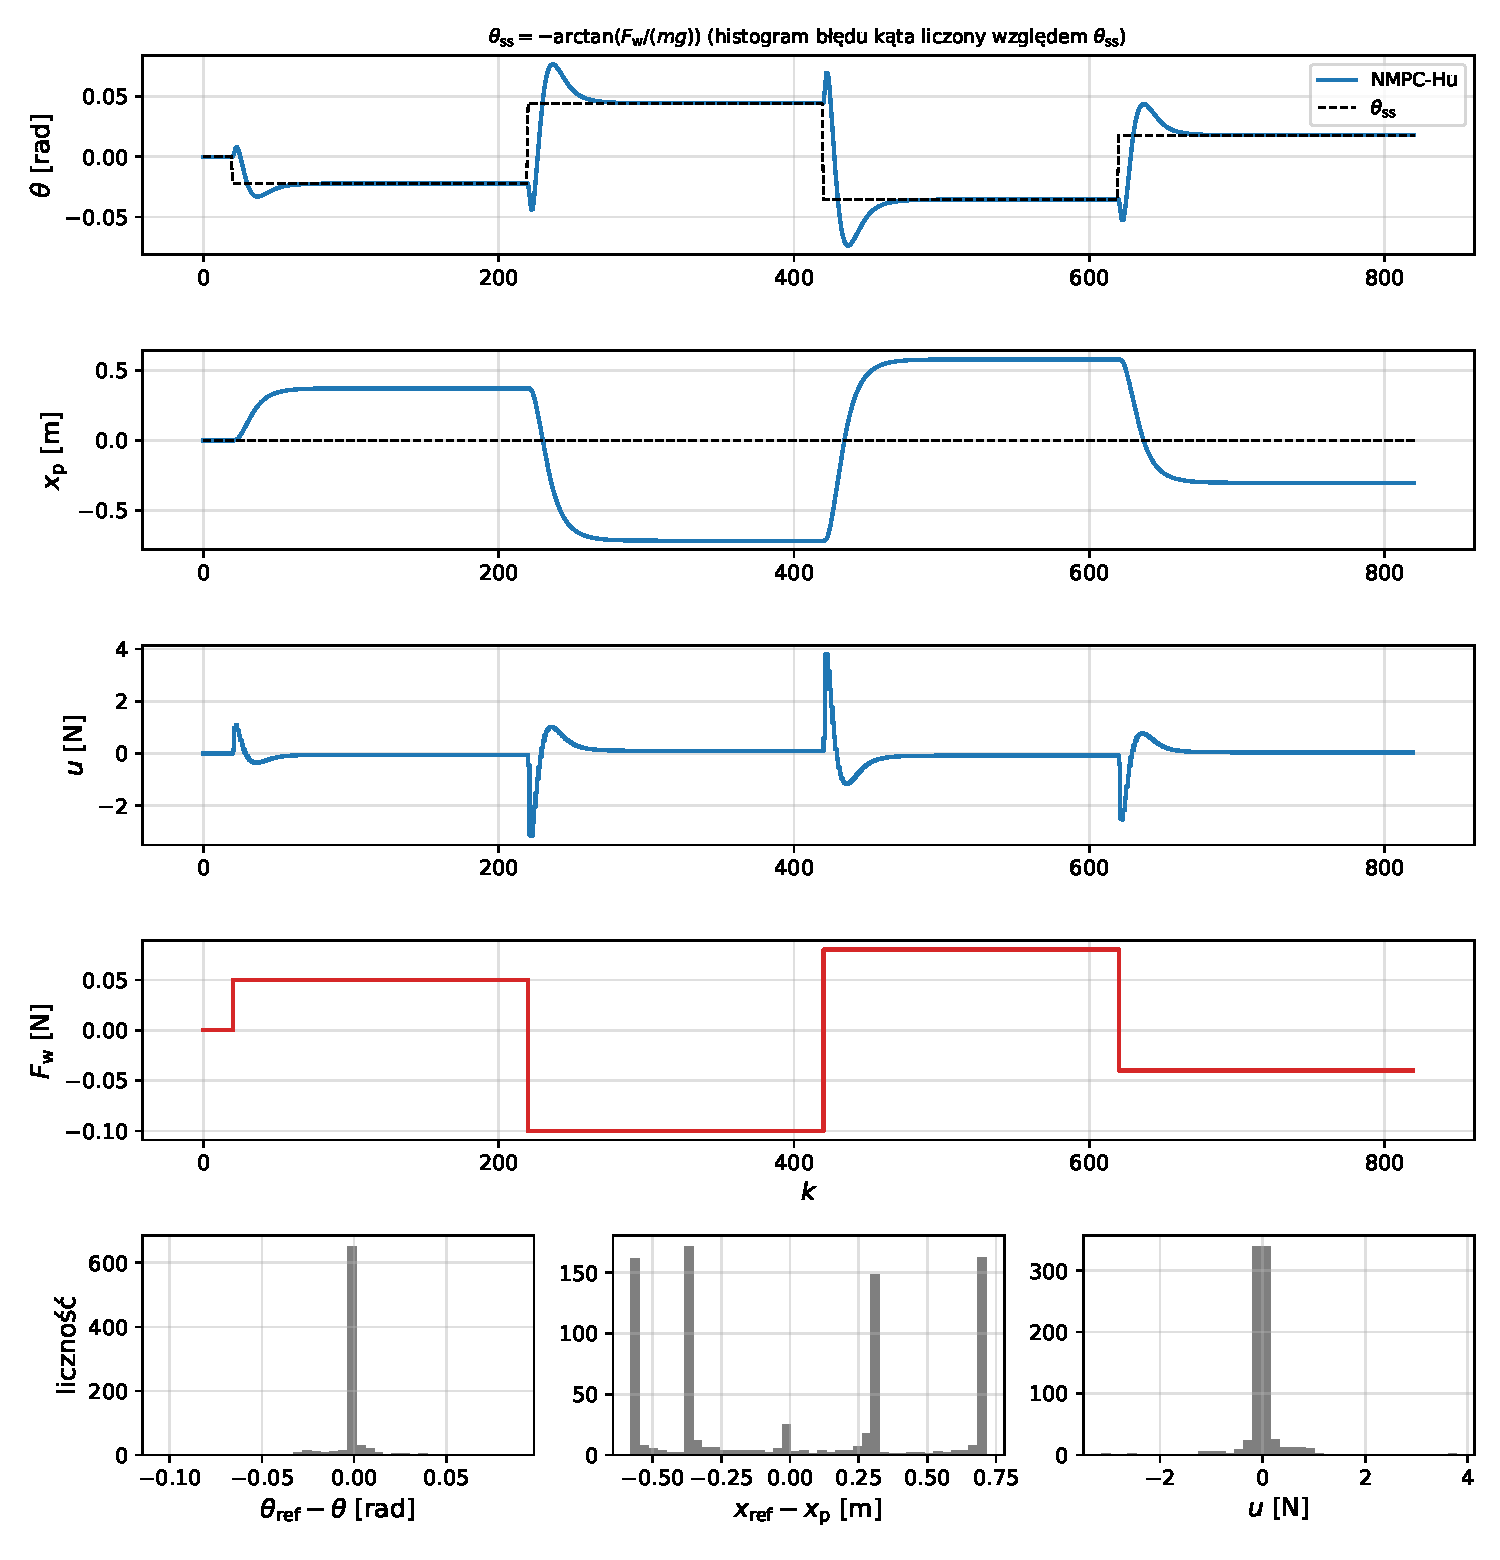
\includegraphics[width=\linewidth]{figs/S2_nmpc_hu.pdf}
\caption{NMPC-Hu, Scenariusz S2 (skoki zakłócenia): status automatyczny -- stabilny.}
\end{figure}
\clearpage
\begin{figure}[p]\centering
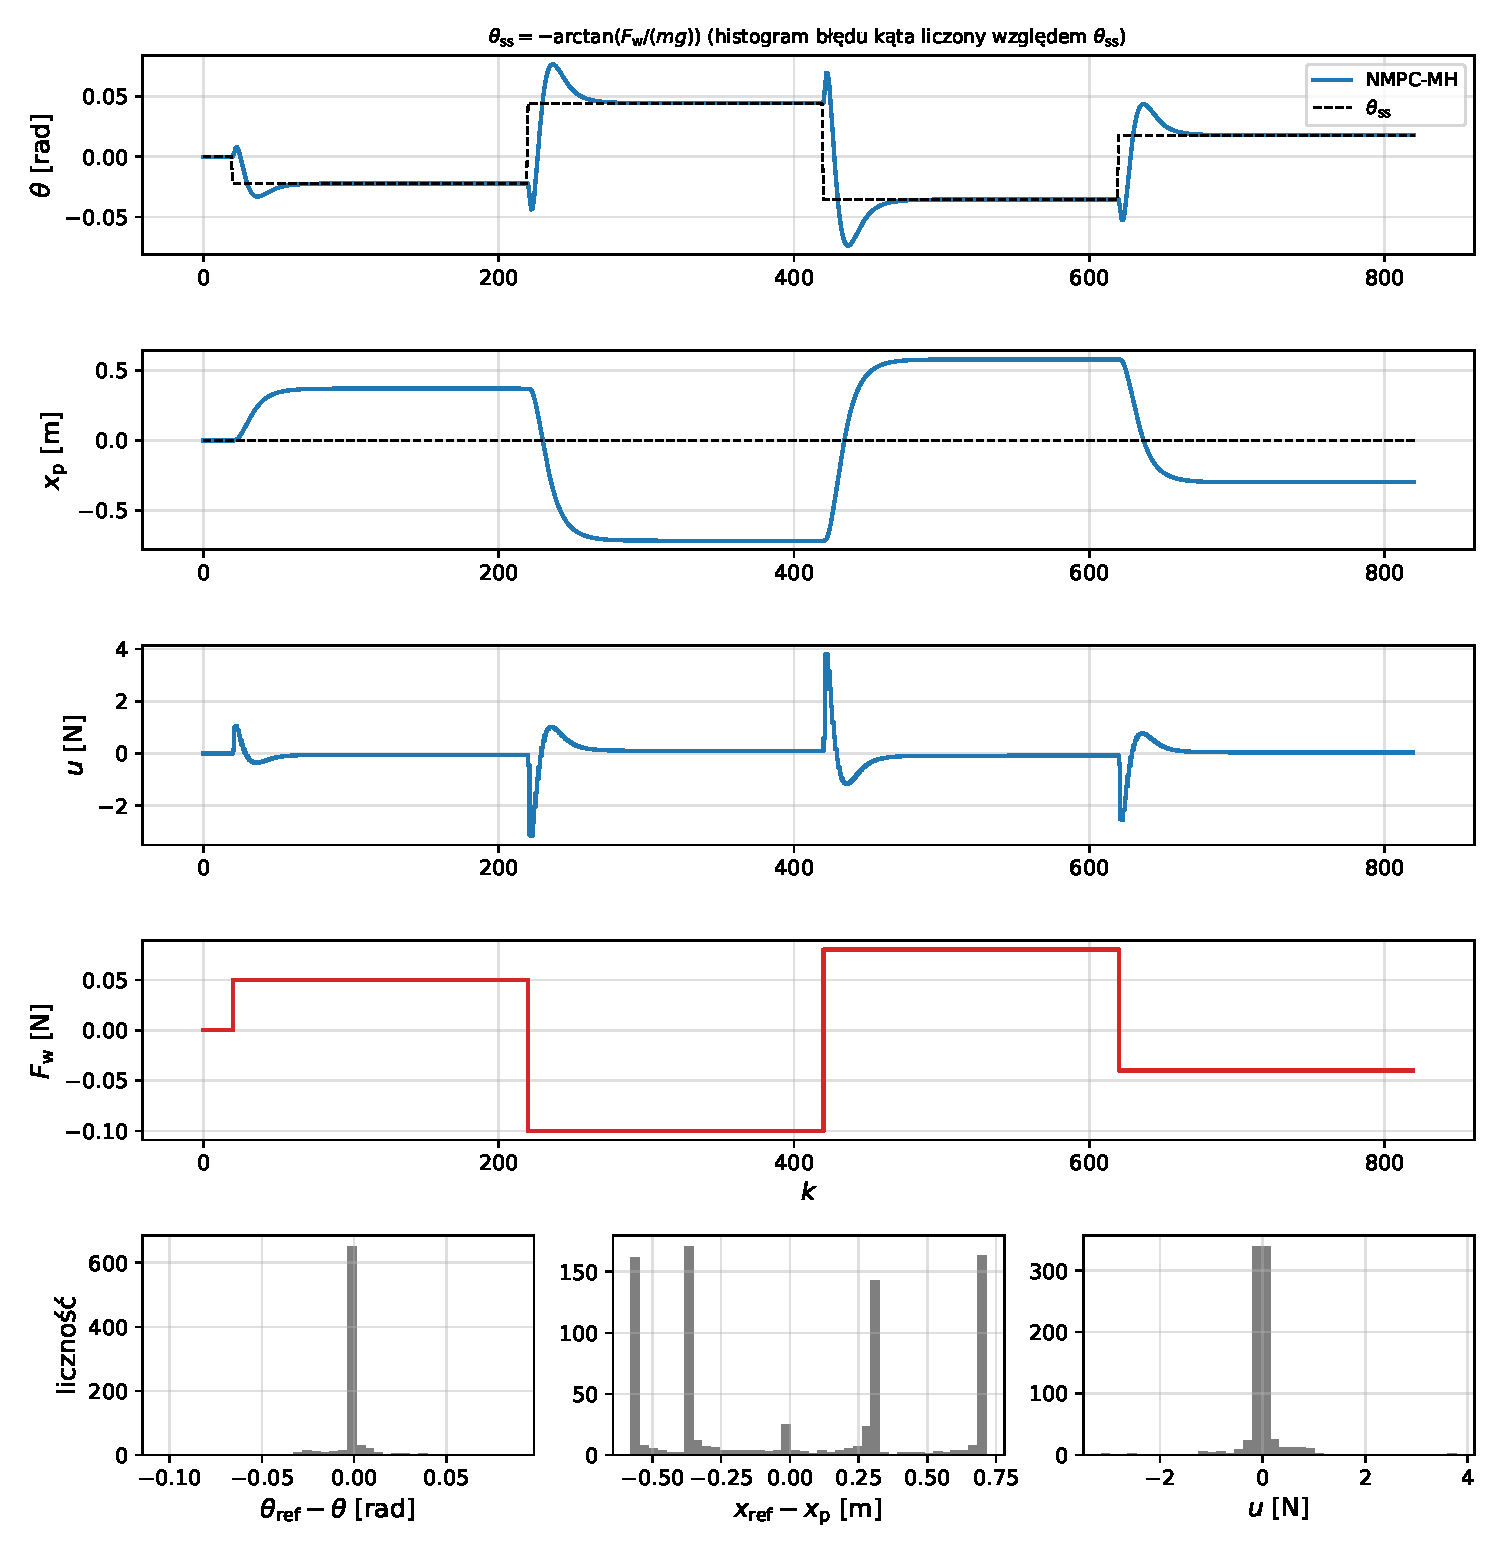
\includegraphics[width=\linewidth]{figs/S2_nmpc_mh.pdf}
\caption{NMPC-MH, Scenariusz S2 (skoki zakłócenia): status automatyczny -- stabilny.}
\end{figure}
\clearpage
\begin{figure}[p]\centering
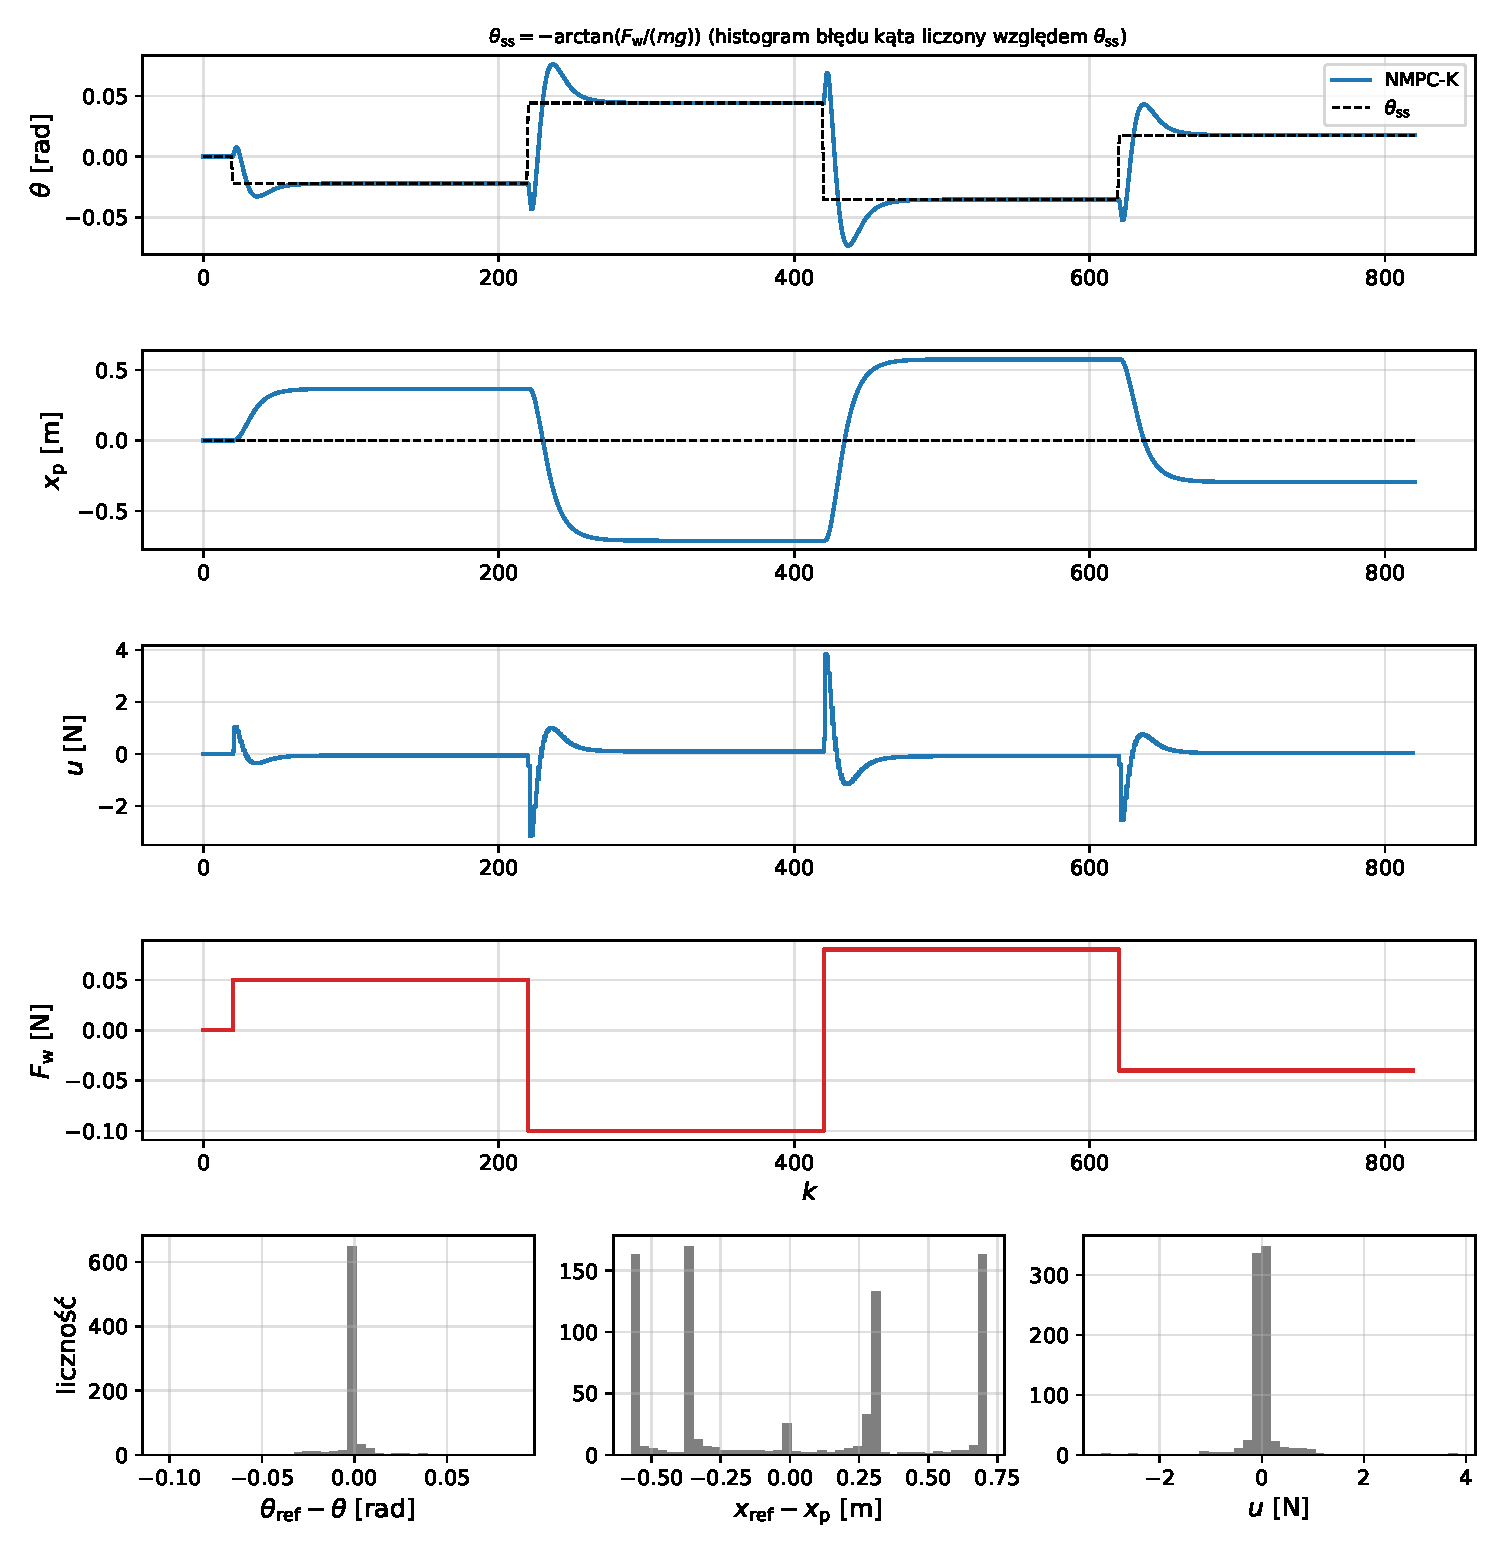
\includegraphics[width=\linewidth]{figs/S2_nmpc_k.pdf}
\caption{NMPC-K, Scenariusz S2 (skoki zakłócenia): status automatyczny -- stabilny.}
\end{figure}
\clearpage
\begin{figure}[p]\centering
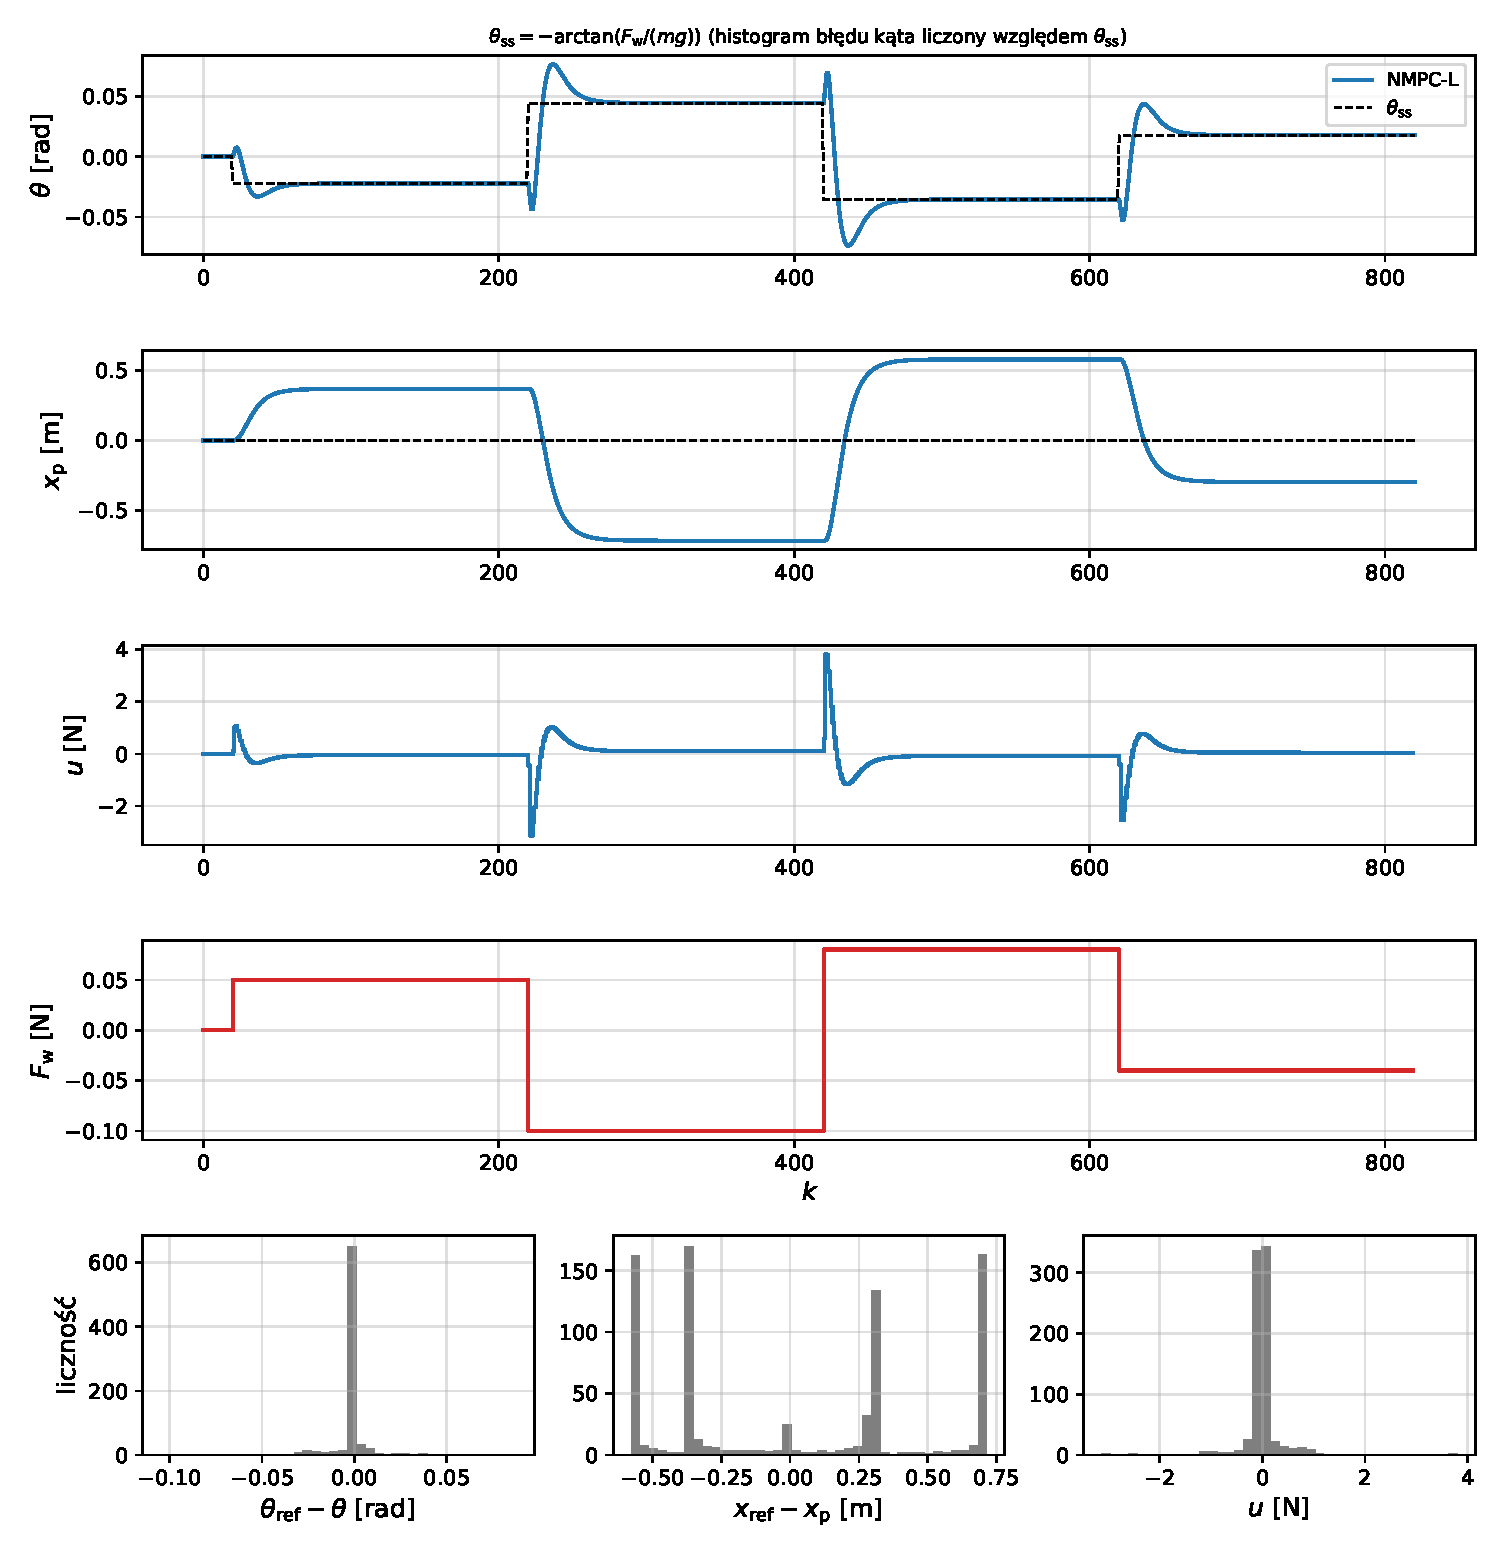
\includegraphics[width=\linewidth]{figs/S2_nmpc_l.pdf}
\caption{NMPC-L, Scenariusz S2 (skoki zakłócenia): status automatyczny -- stabilny.}
\end{figure}
\clearpage
\begin{figure}[p]\centering
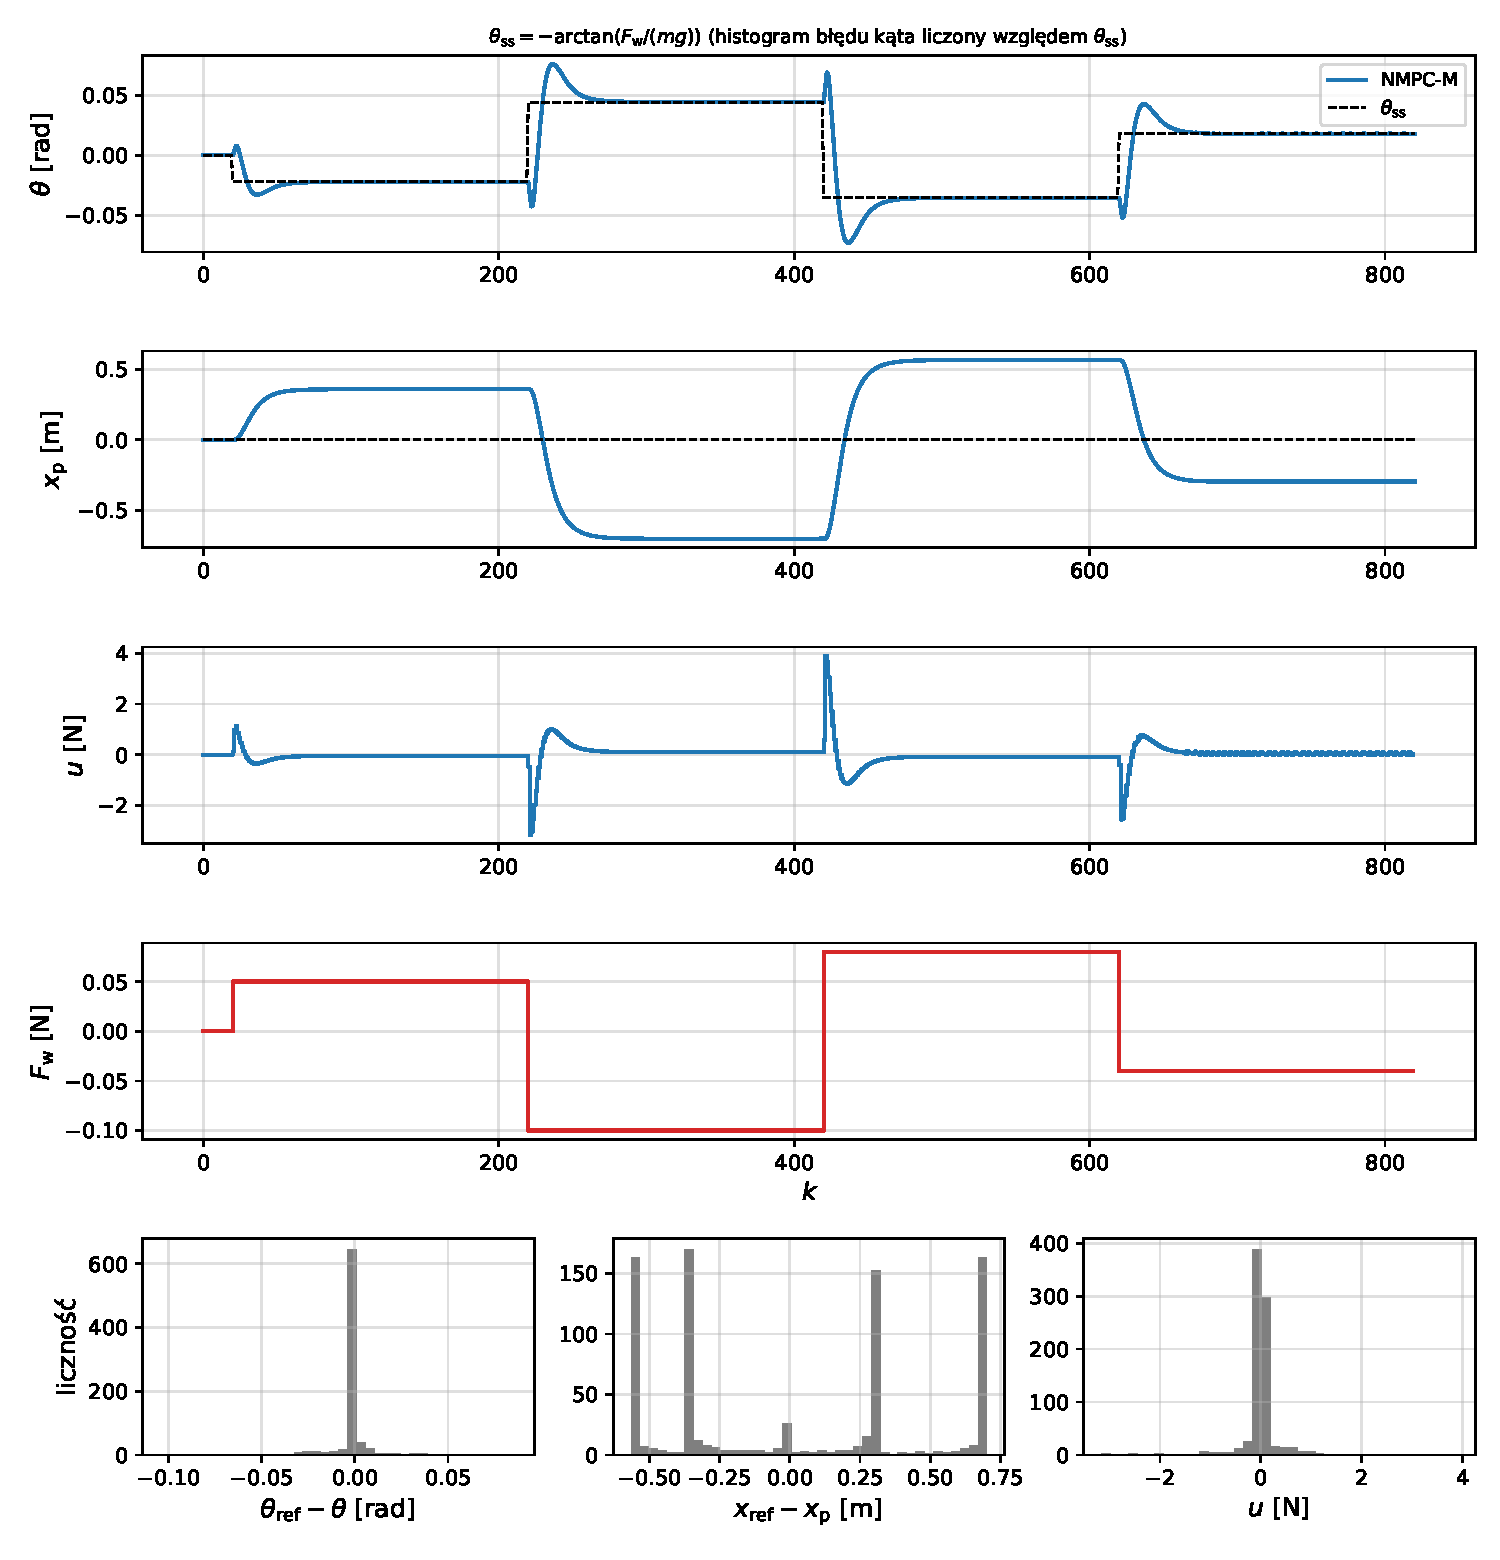
\includegraphics[width=\linewidth]{figs/S2_nmpc_m.pdf}
\caption{NMPC-M, Scenariusz S2 (skoki zakłócenia): status automatyczny -- stabilny.}
\end{figure}
\clearpage
\begin{figure}[p]\centering
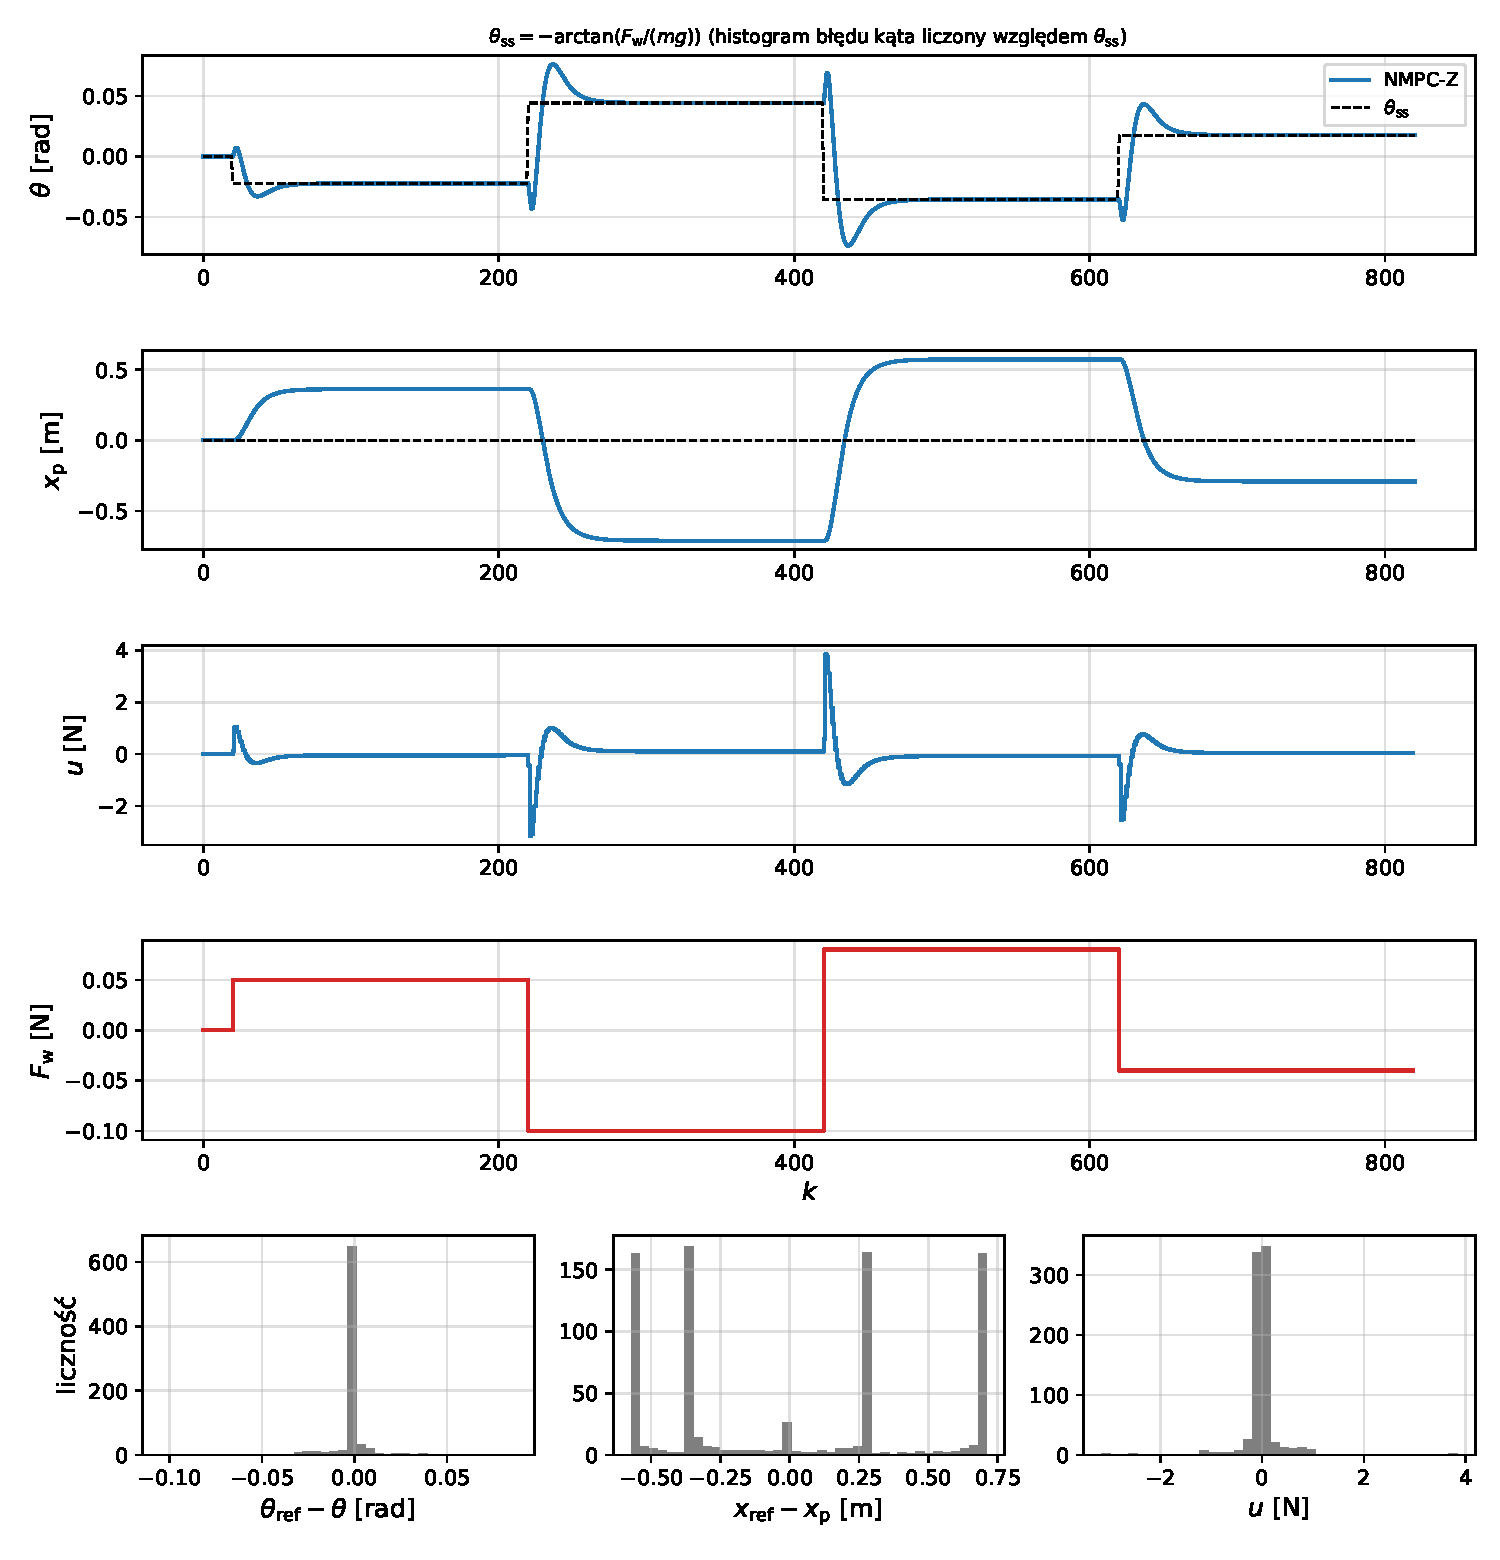
\includegraphics[width=\linewidth]{figs/S2_nmpc_z.pdf}
\caption{NMPC-Z, Scenariusz S2 (skoki zakłócenia): status automatyczny -- stabilny.}
\end{figure}
\clearpage
\begin{figure}[p]\centering
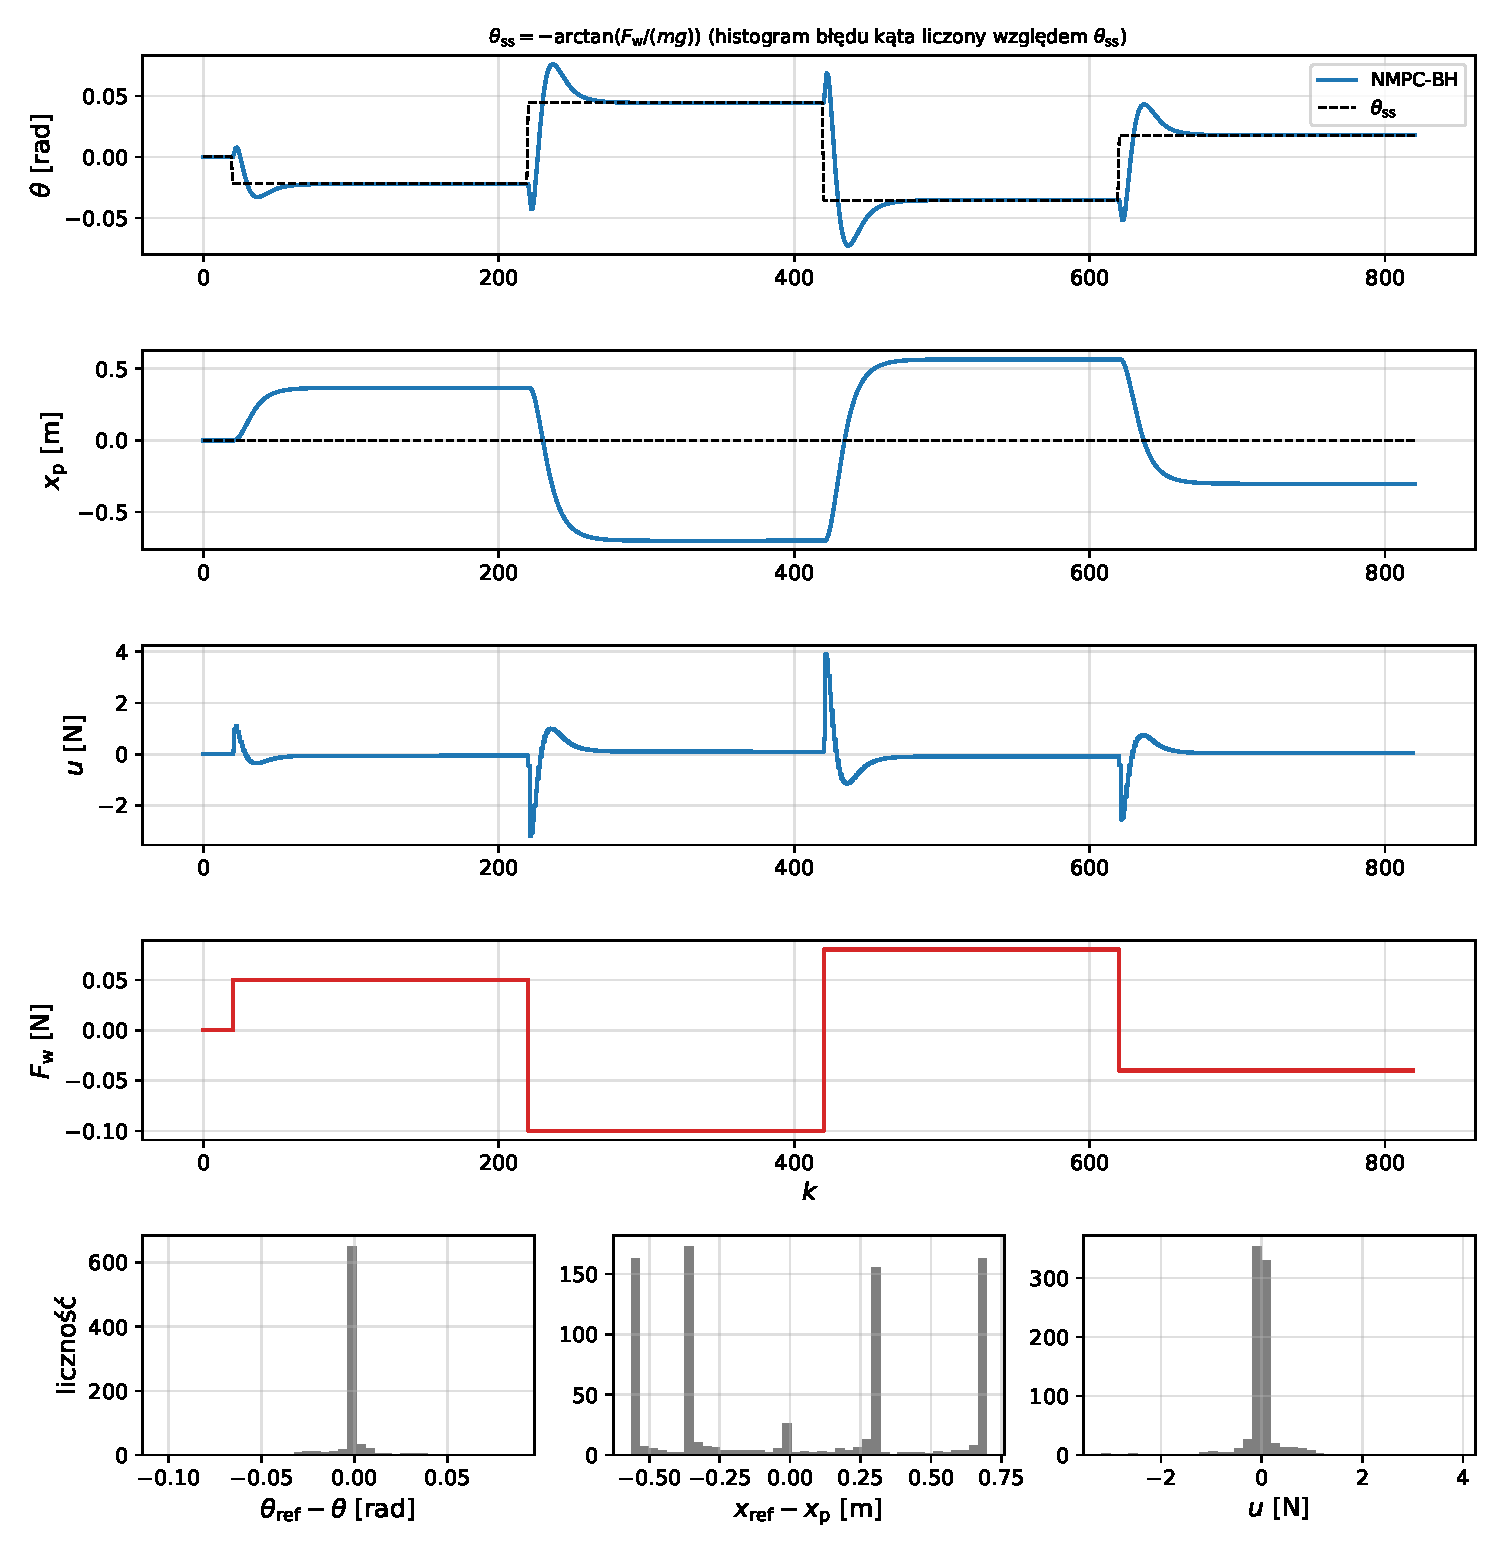
\includegraphics[width=\linewidth]{figs/S2_nmpc_bh.pdf}
\caption{NMPC-BH, Scenariusz S2 (skoki zakłócenia): status automatyczny -- stabilny.}
\end{figure}
\clearpage
\begin{figure}[p]\centering
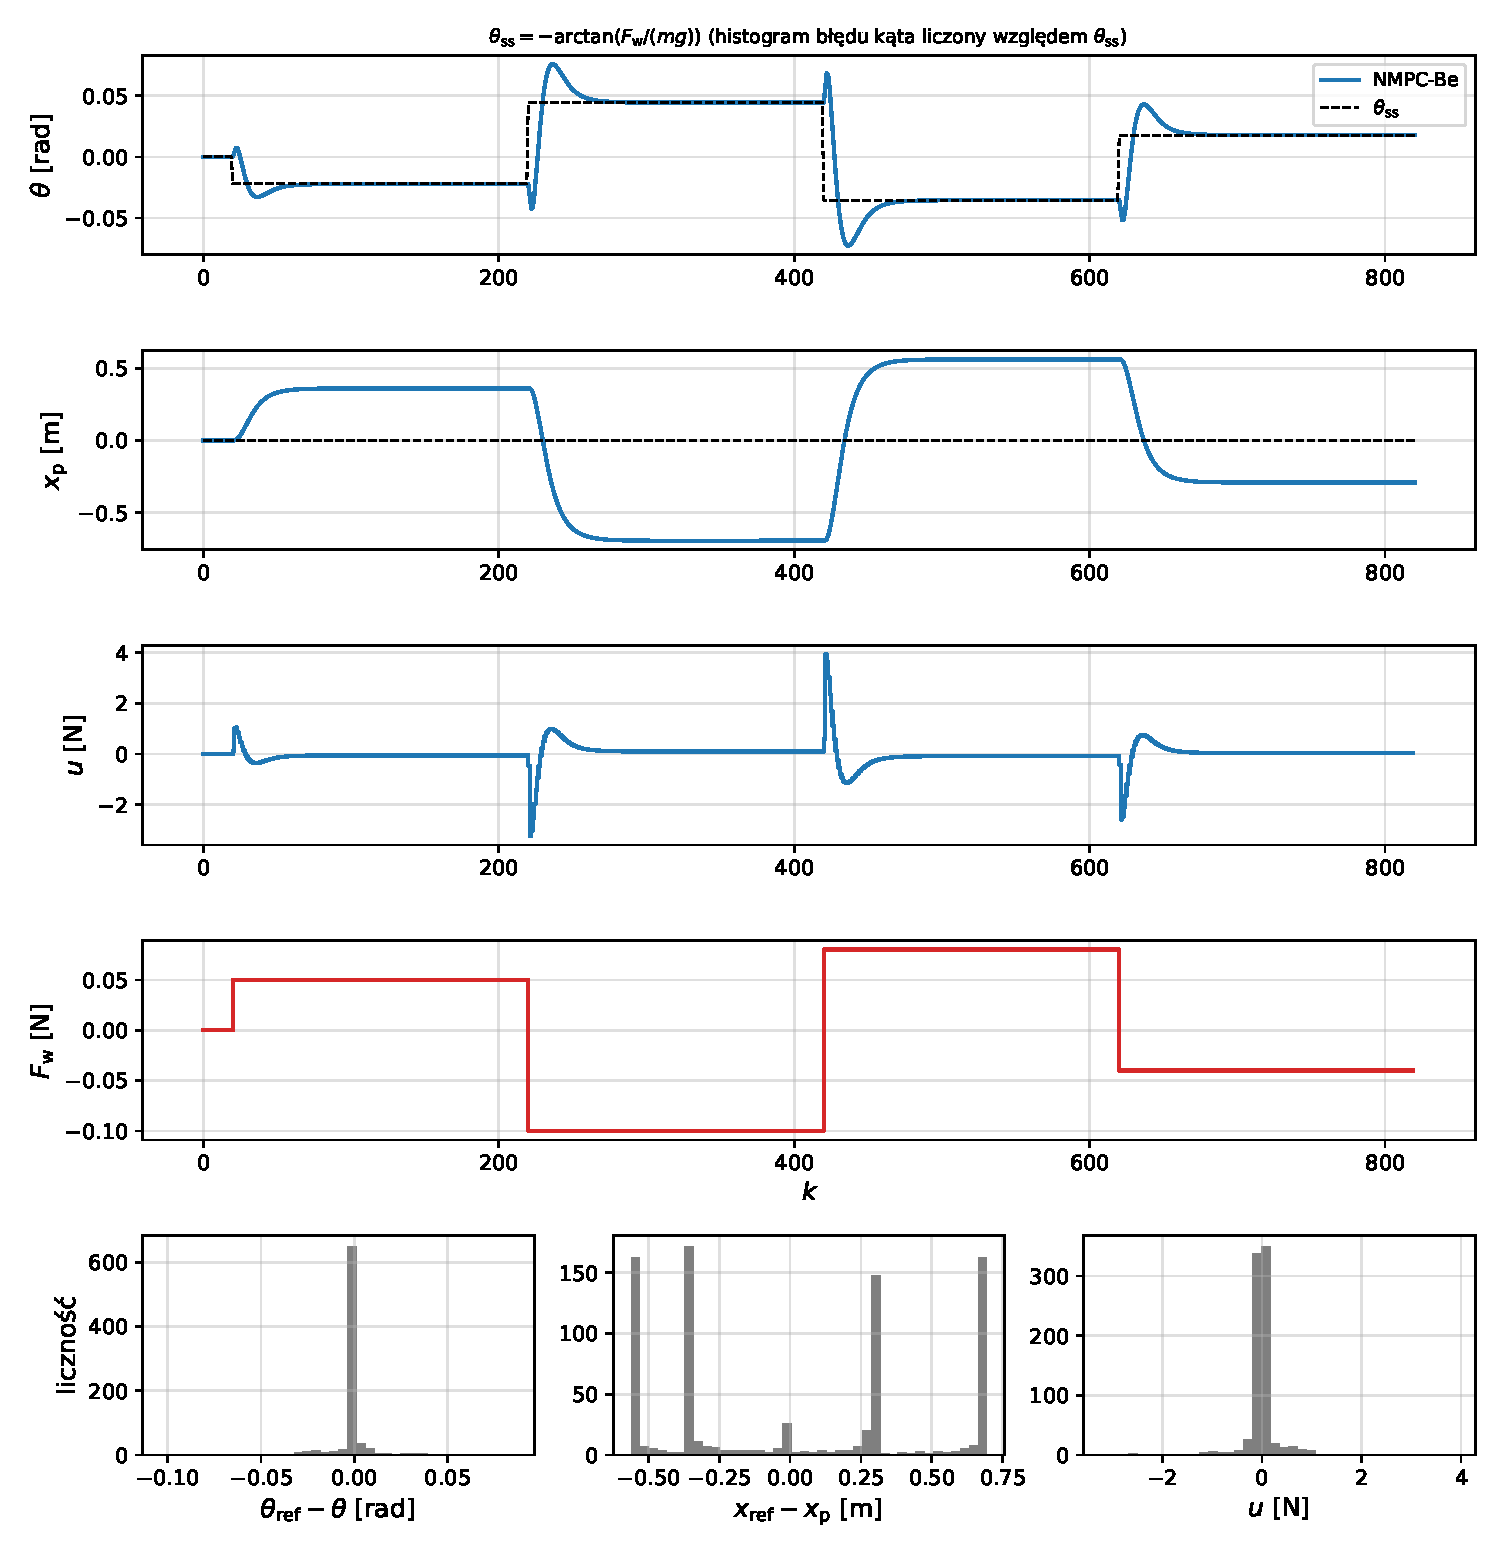
\includegraphics[width=\linewidth]{figs/S2_nmpc_be.pdf}
\caption{NMPC-Be, Scenariusz S2 (skoki zakłócenia): status automatyczny -- stabilny.}
\end{figure}
\clearpage
\begin{figure}[p]\centering
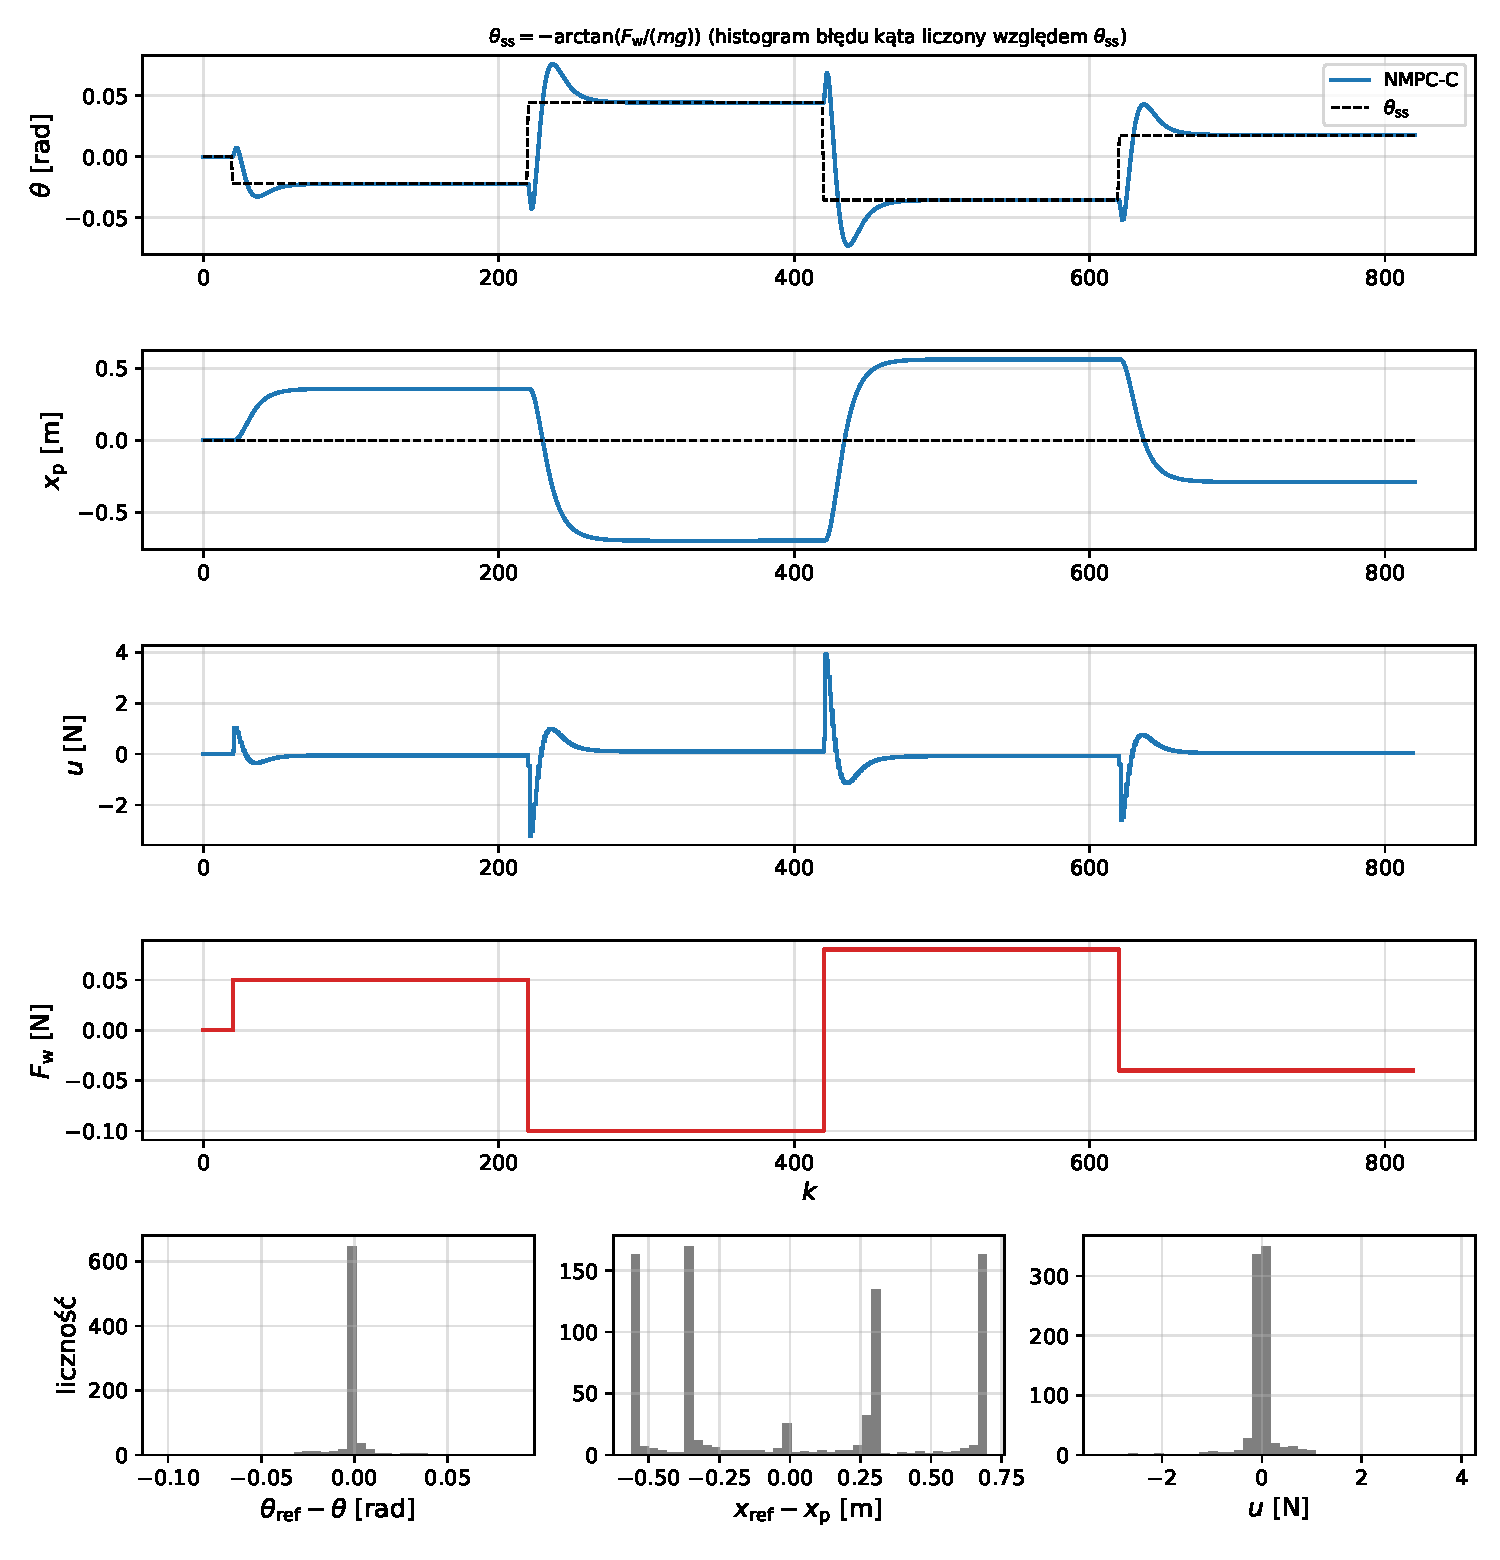
\includegraphics[width=\linewidth]{figs/S2_nmpc_c.pdf}
\caption{NMPC-C, Scenariusz S2 (skoki zakłócenia): status automatyczny -- stabilny.}
\end{figure}
\clearpage
\begin{figure}[p]\centering
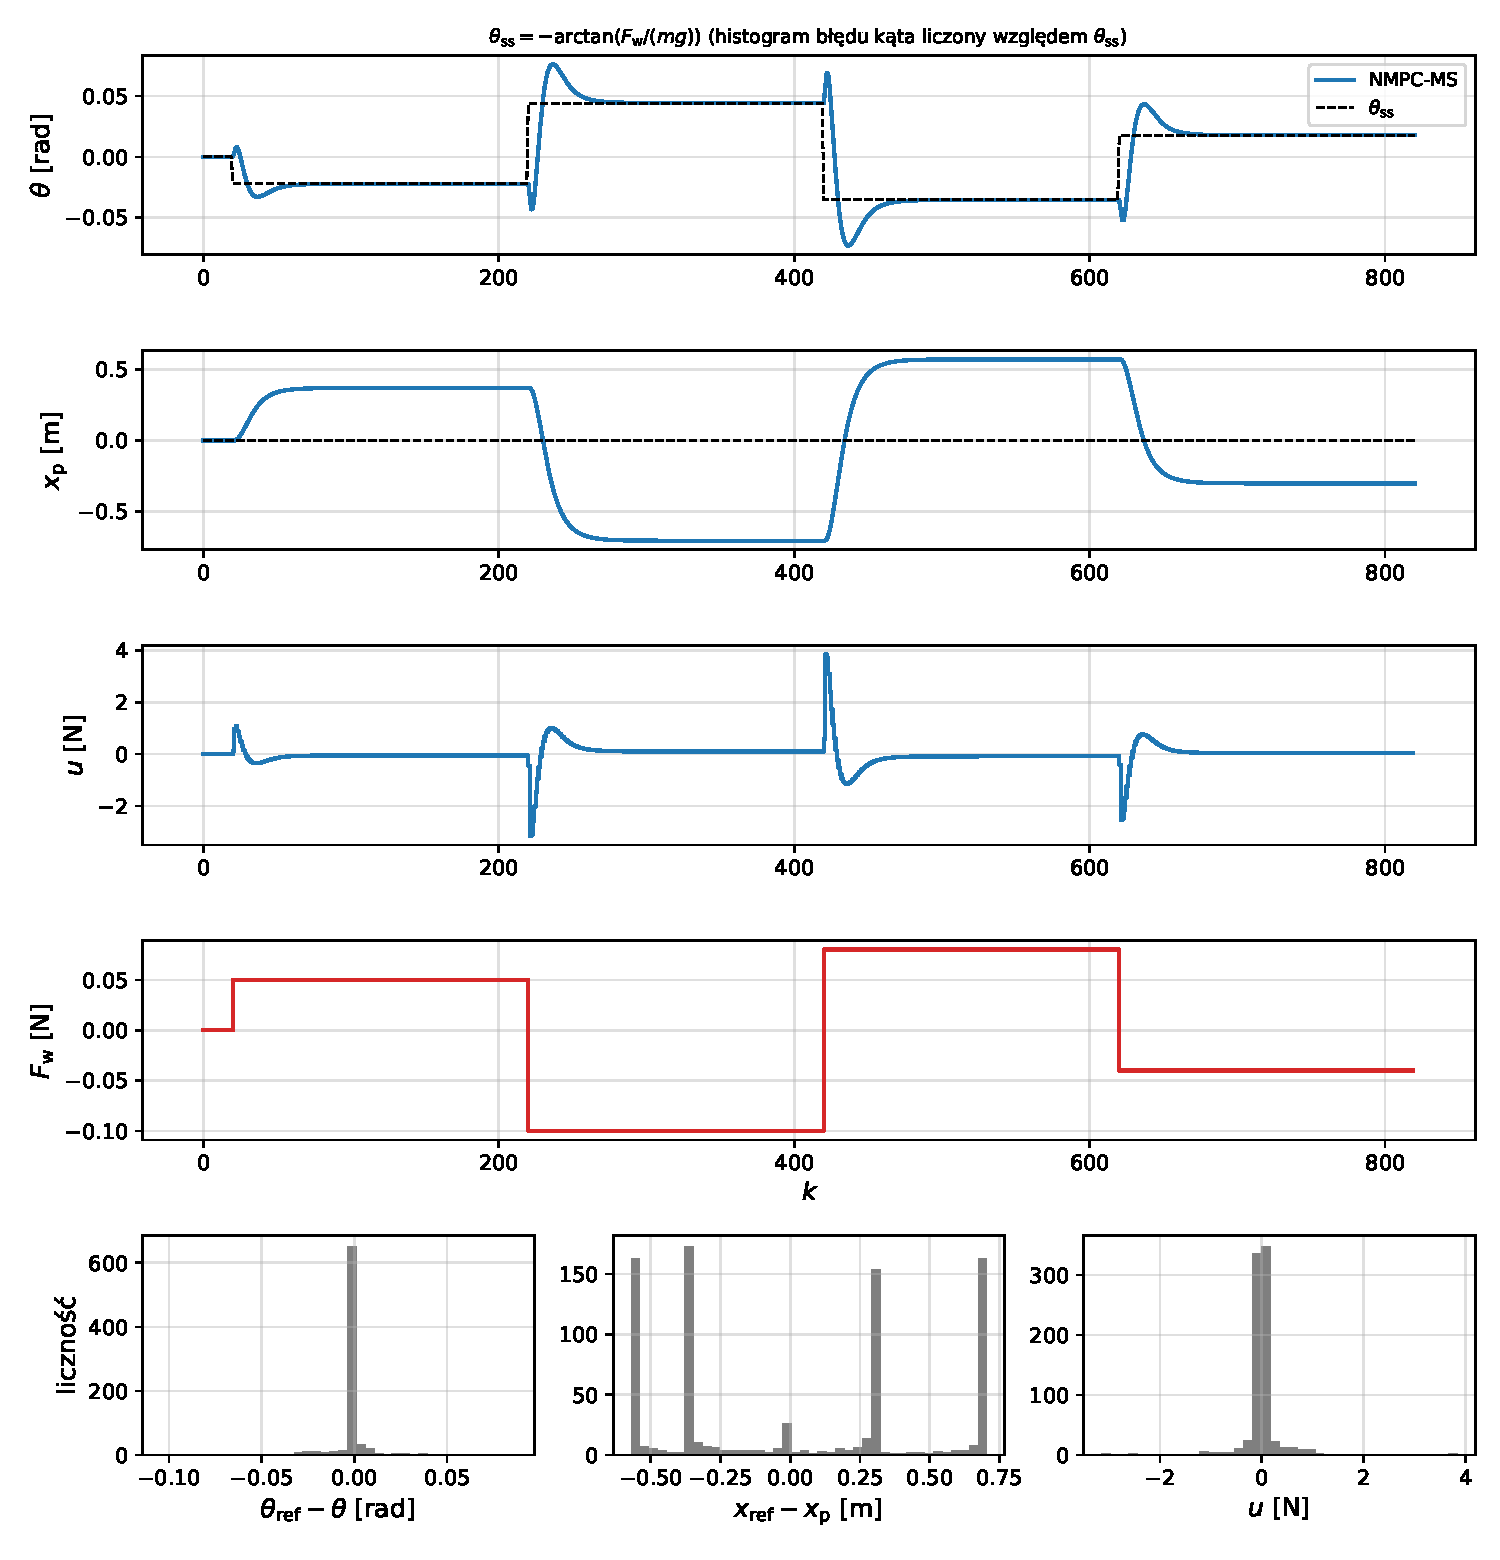
\includegraphics[width=\linewidth]{figs/S2_nmpc_ms.pdf}
\caption{NMPC-MS, Scenariusz S2 (skoki zakłócenia): status automatyczny -- stabilny.}
\end{figure}
\clearpage
\begin{figure}[p]\centering
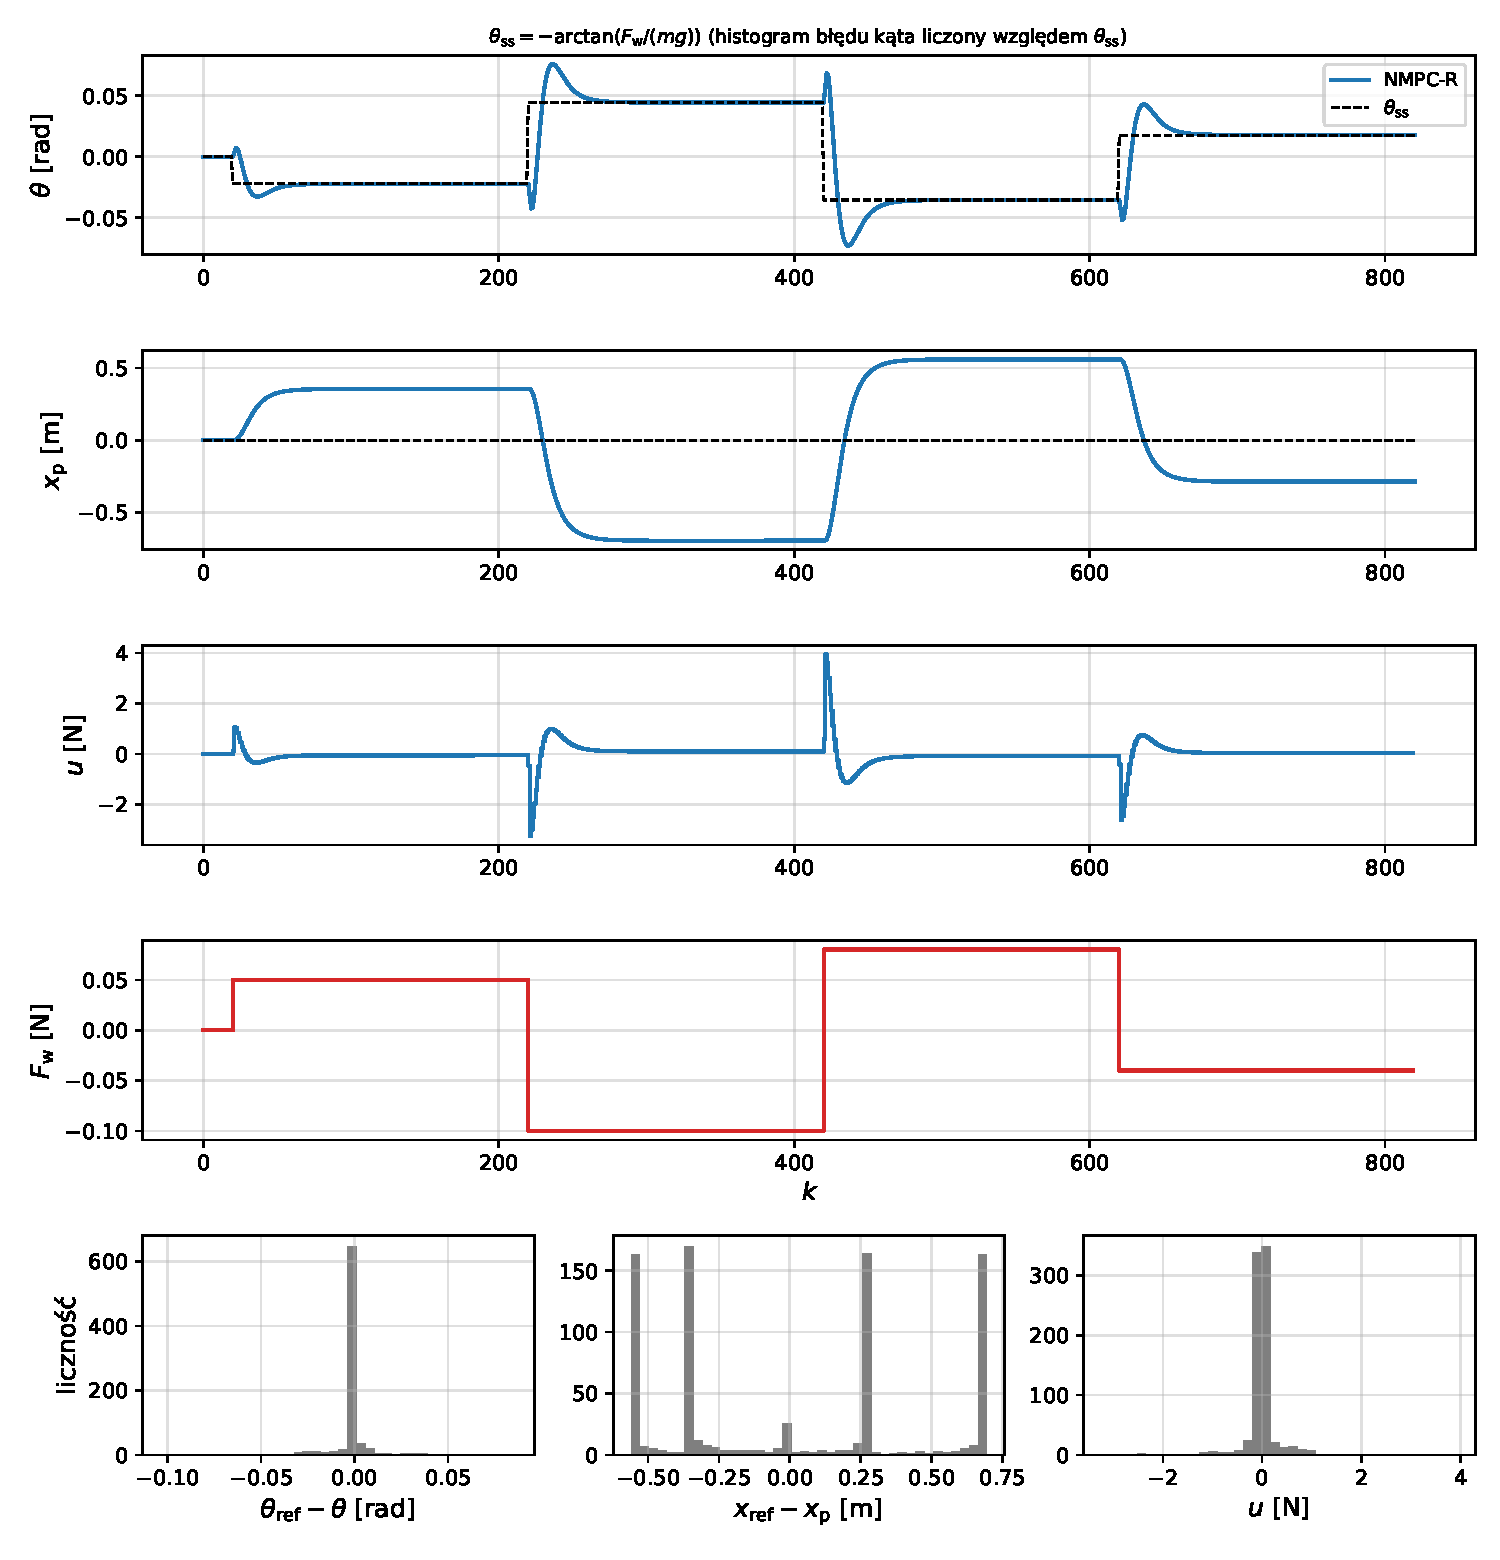
\includegraphics[width=\linewidth]{figs/S2_nmpc_r.pdf}
\caption{NMPC-R, Scenariusz S2 (skoki zakłócenia): status automatyczny -- stabilny.}
\end{figure}
\clearpage
\begin{figure}[p]\centering
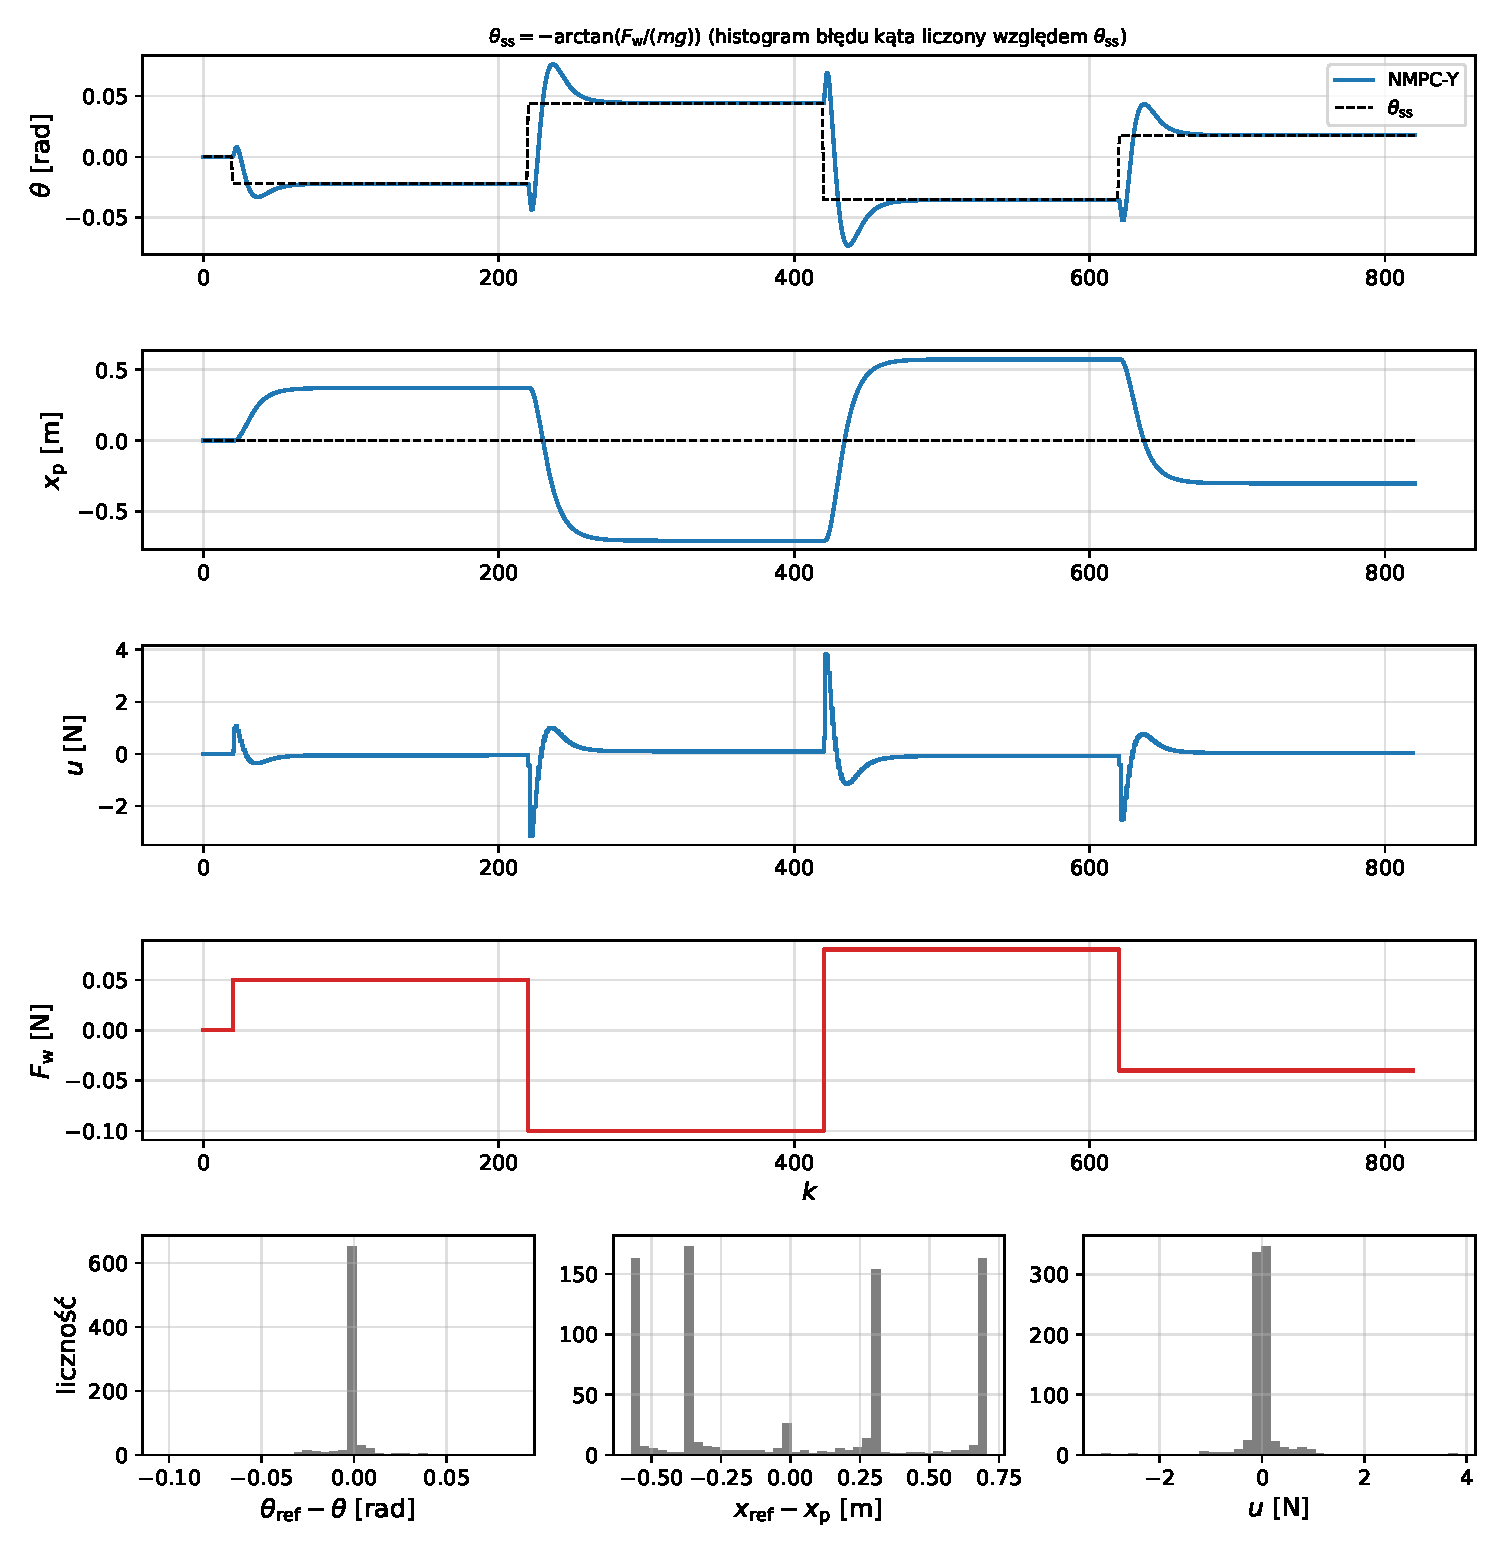
\includegraphics[width=\linewidth]{figs/S2_nmpc_y.pdf}
\caption{NMPC-Y, Scenariusz S2 (skoki zakłócenia): status automatyczny -- stabilny.}
\end{figure}
\clearpage


\end{document}
